\documentclass[11pt,a5paper,twoside]{book}
\usepackage[utf8]{inputenc}
\usepackage[spanish]{babel}
\usepackage[T1]{fontenc}
\usepackage{lmodern}
\usepackage{microtype}
\usepackage{geometry}
\geometry{
    a5paper,
    inner=25mm,
    outer=20mm,
    top=20mm,
    bottom=20mm
}
\usepackage{graphicx}
\usepackage{titlesec}
\titleformat{\chapter}[display]
  {\normalfont\huge\bfseries\raggedright}{\chaptertitlename\ \thechapter}{20pt}{\Huge}
\usepackage[titles]{tocloft}
\setlength{\cftchapnumwidth}{3.5em}
\widowpenalty=10000
\clubpenalty=10000
\linespread{1.15}
\usepackage{fancyhdr}
\pagestyle{fancy}
\fancyhf{}
\fancyfoot[L]{\thepage}
\fancyfoot[R]{\rightmark}
\renewcommand{\headrulewidth}{0pt}
\renewcommand{\footrulewidth}{0pt}
\renewcommand{\thechapter}{\Roman{chapter}}
\title{Bitácora Centauri \\ \large Diario de un documentalista técnico}
\author{IOREB}
\date{}

\begin{document}

\newgeometry{margin=0pt}
\thispagestyle{empty}
\noindent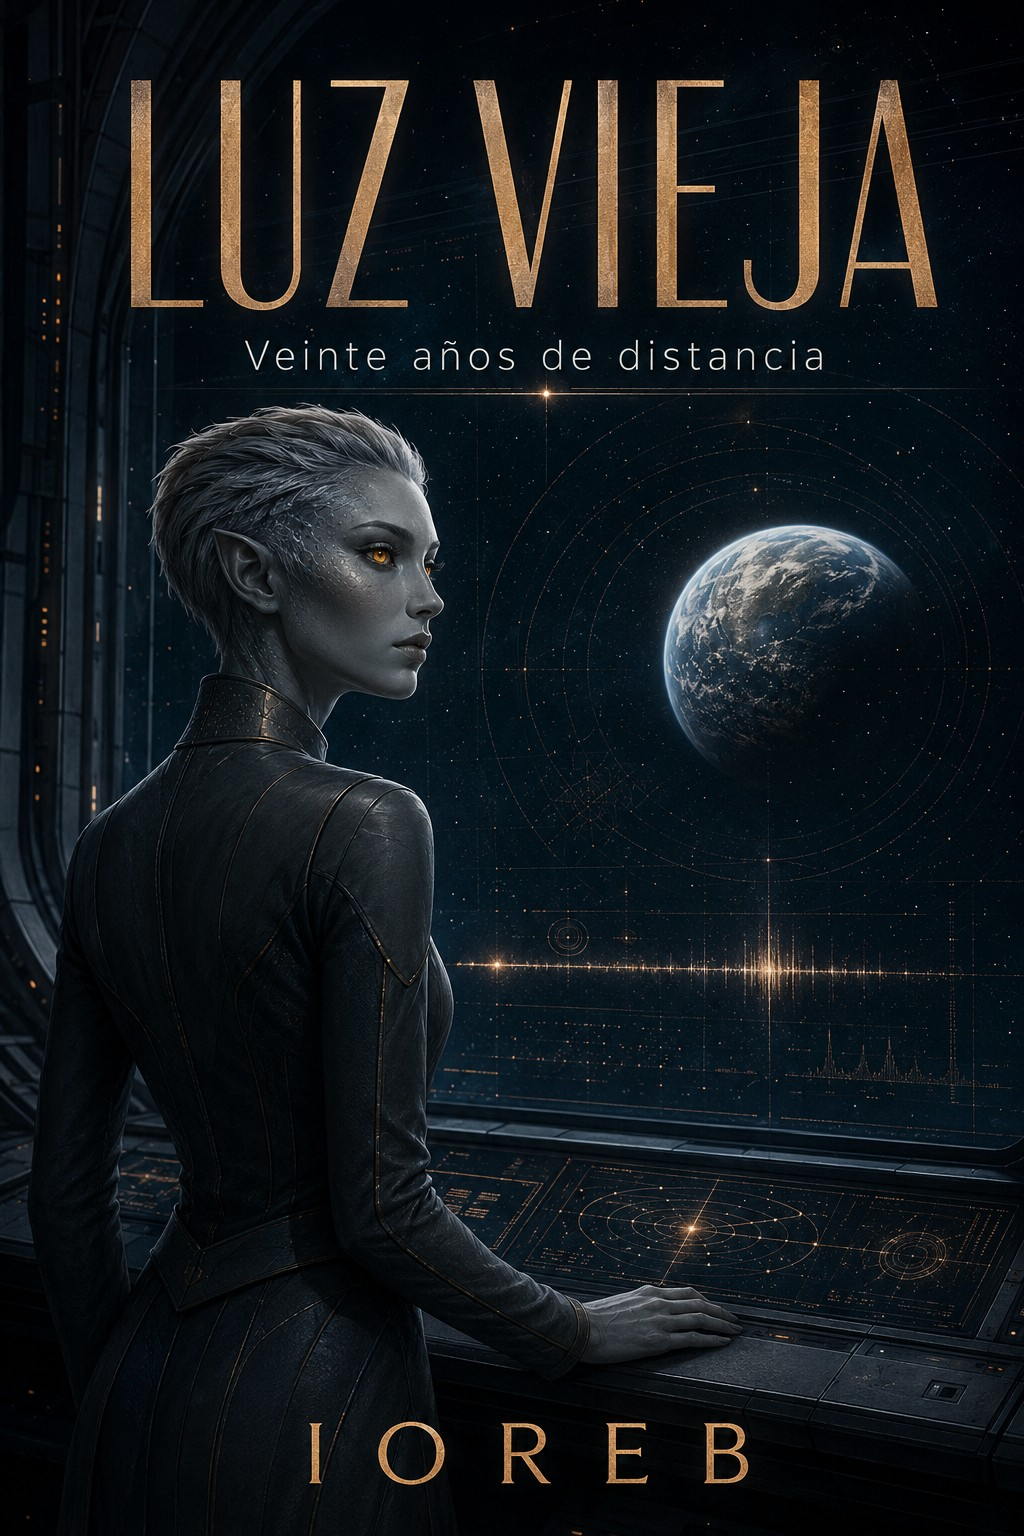
\includegraphics[width=\paperwidth, height=\paperheight]{portada.jpg}
\clearpage
\restoregeometry

\frontmatter
\maketitle
\clearpage
\thispagestyle{empty}
\vspace*{\fill}
\begin{center}
{\small
\textbf{Bitácora Centauri} \\
Autor: IOREB \\
© 2026, IOREB. Todos los derechos reservados. \\
\vspace{1.5em}
Cualquier forma de reproducción, distribución, comunicación pública o transformación de esta obra solo puede ser realizada con la autorización de sus titulares, salvo excepción prevista por la ley. Diríjase a CEDRO (Centro Español de Derechos Reprográficos) si necesita fotocopiar o escanear algún fragmento de esta obra. \\
\vspace{1.5em}
Diseño de portada: IOREB. \\
\vspace{1.5em}
Declaración de Asistencia de IA: Esta obra de ciencia ficción ha sido desarrollada y traducida con la asistencia de modelos de lenguaje de inteligencia artificial como parte de un proceso creativo agéntico iterativo en EditorIAl IOREB.
}
\end{center}
\vspace*{\fill}
\clearpage
\tableofcontents

\mainmatter
\chapter*{Prólogo — Tierra}
\addcontentsline{toc}{chapter}{Prólogo — Tierra}
\markboth{Prólogo — Tierra}{Prólogo — Tierra}

*\textit{Día 0. Estación LEO. Órbita baja terrestre.}*

La última noche en la Tierra no dormí.

No por miedo. O no solo por miedo.

Me quedé sentado junto a la ventana del apartamento orbital de espera, mirando el planeta bajo mis pies. Desde la Estación LEO, la Tierra no parecía el lugar donde uno había vivido toda la vida, sino algo imposible de abandonar sin sentirse culpable. Una esfera azul, blanca y oscura, con tormentas moviéndose lentamente sobre los océanos y ciudades encendidas como brasas.

\begin{figure}[h]
\centering
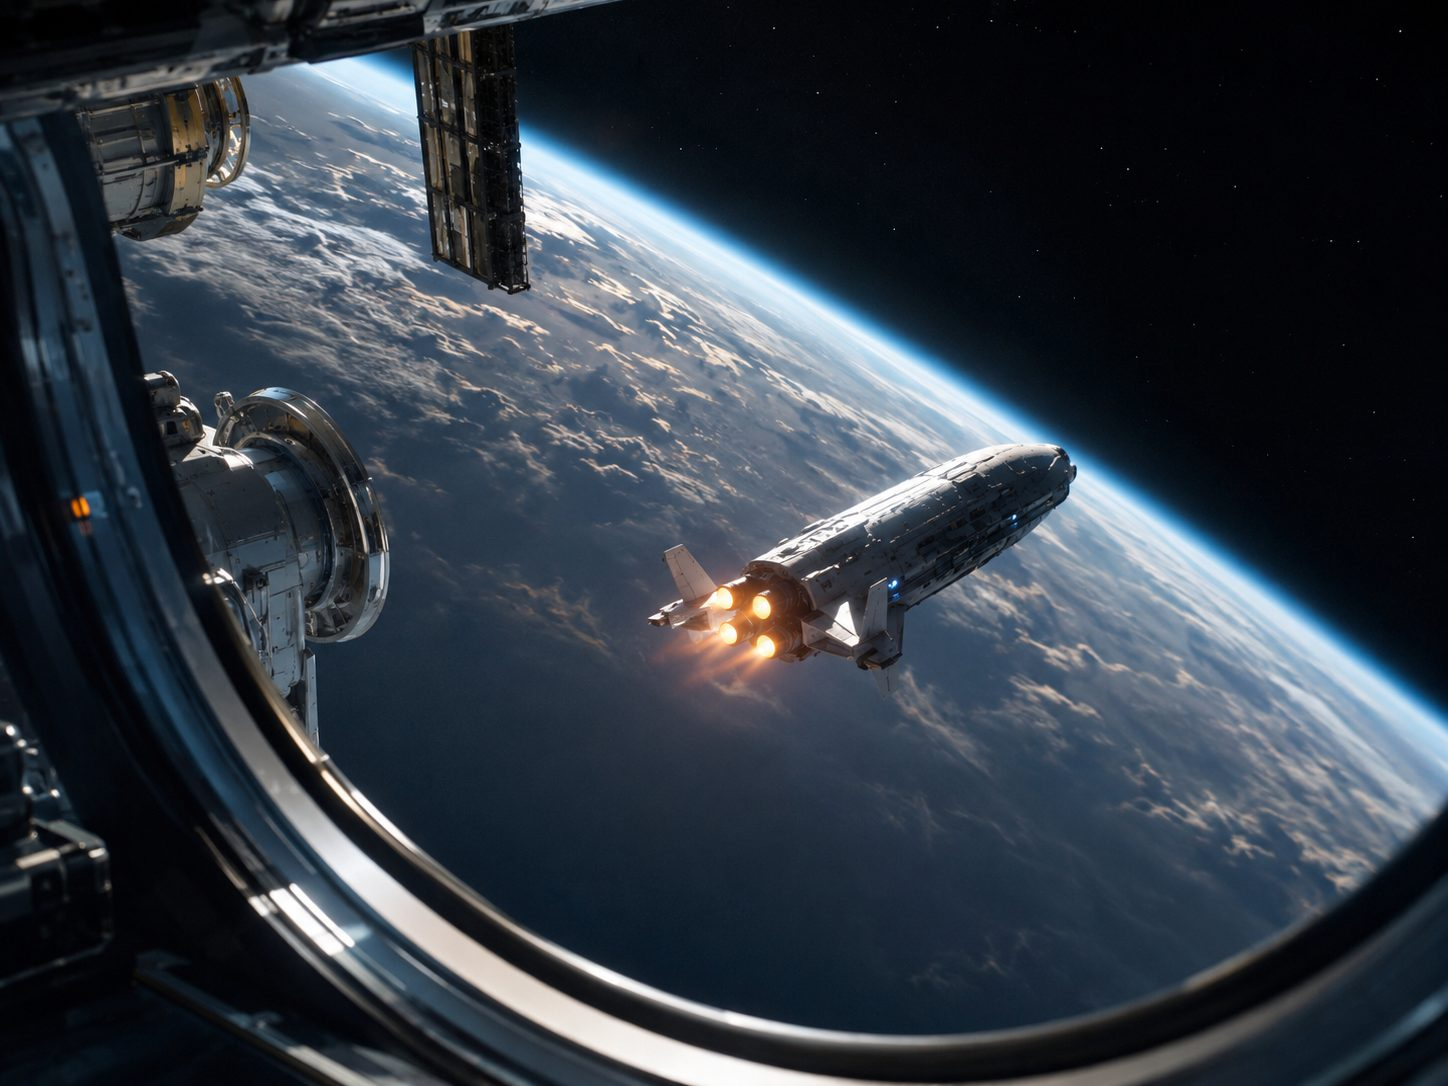
\includegraphics[width=0.9\textwidth]{00_1_vistaespacialdesdeunaestacinorbital.jpg}
\end{figure}

Aragón, Madrid, el Mediterráneo, África… Todo estaba allí abajo, pero ya no podía señalar nada con precisión. La escala humana había desaparecido. Cuatrocientos kilómetros de vacío convierten los lugares en conceptos.

Había gente durmiendo en los módulos contiguos. Los escuchaba moverse, cambiar de postura, murmurar algo. Nadie más estaba mirando por la ventana a esa hora. Tal vez lo habían hecho el primer día y ya les había parecido suficiente. Yo llevaba tres noches así, despierto ante el planeta, intentando memorizarlo de una manera que las fotografías no podían sustituir.

El problema es que la memoria funciona con escala humana. Y desde aquí, la Tierra no tenía escala humana. Tenía la escala de algo que no cabe en la cabeza.

En la pantalla del módulo apareció el aviso:

\begin{figure}[h]
\centering
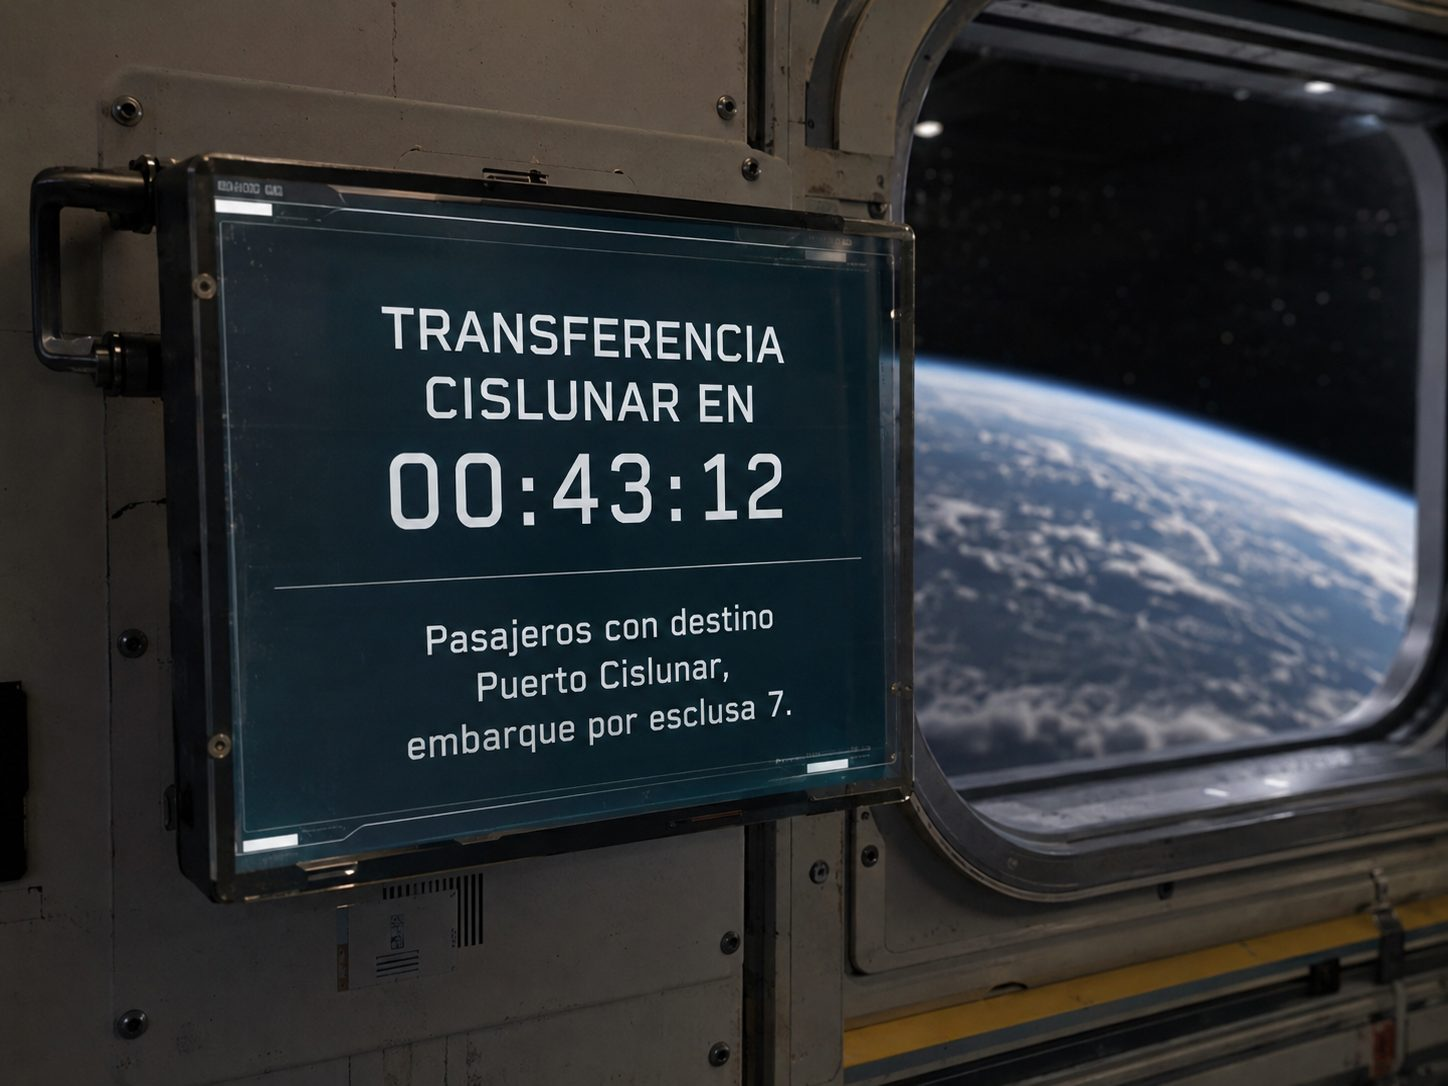
\includegraphics[width=0.9\textwidth]{00_2_pantalladetransferenciaenlanave.jpg}
\end{figure}

> TRANSFERENCIA CISLUNAR EN 00:43:12
> Pasajeros con destino Puerto Cislunar, embarque por esclusa 7.

La fuente era la misma que usaban los avisos de tren. Alguien, en algún momento del diseño del sistema, había decidido que el formato de los avisos del primer trayecto interestelar debería parecer el de una estación de ferrocarril. Me pareció una decisión completamente sensata.

Así empezó mi viaje a *\textit{Nueva Concordia}\textit{, la primera colonia permanente en construcción alrededor de }\textit{Alpha Centauri A}*.

No iba en misión oficial. No era piloto, ni ingeniero de campo, ni diplomático. Era documentalista técnico: mi trabajo consistía en narrar el viaje completo para los archivos de colonización. Había pedido el encargo yo mismo, con un argumento que convencí a los comités en tres frases: que el viaje largo era el viaje real, que los datos técnicos ya los tenían, y que lo que no tenían era alguien que mirara por la ventana.

La mayoría de pasajeros tomaban el itinerario rápido: Tierra, Puerto Cislunar, catapulta interior, Estación Warp Exterior, lanzamiento. Dieciséis días desde la LEO hasta la Atenea Larga. Limpio, eficiente, sin rodeos.

Pero yo había solicitado el trayecto largo.

Quería verlo todo.

\begin{figure}[h]
\centering
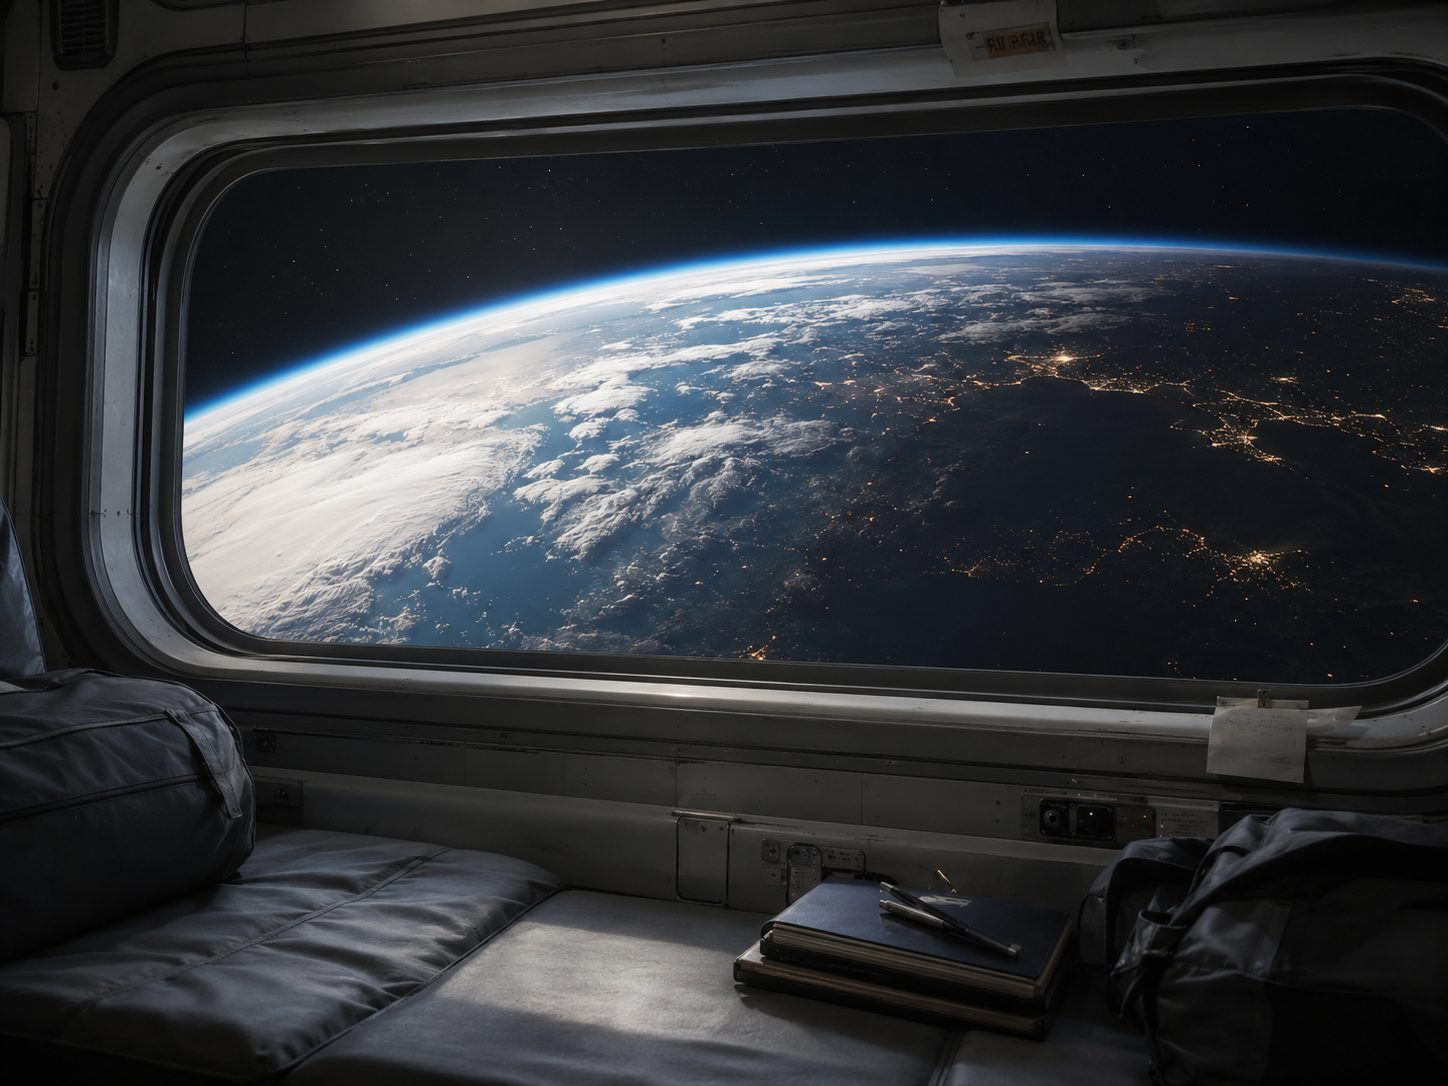
\includegraphics[width=0.9\textwidth]{00_3_vistatranquiladelespacioterrestre.jpg}
\end{figure}

La vieja red de fusión. Los ciclers que aún seguían funcionando. Fobos. Ceres. Calisto. Titán. La gran estación entre Júpiter y Saturno. Quería pasar por cada nodo de la civilización humana antes de saltar hacia el siguiente sol.

Quería entender cómo una especie que apenas había aprendido a salir de su planeta se había atrevido a tender una línea hasta otra estrella.

El aviso parpadeó de nuevo. Cuarenta y dos minutos.

Me levanté. Cogí la bolsa. Antes de salir del módulo, me volví a mirar la ventana una vez más.

La Tierra seguía allí. Enorme. Imposible de caber en ningún recuerdo.

Me fui.

\begin{figure}[h]
\centering
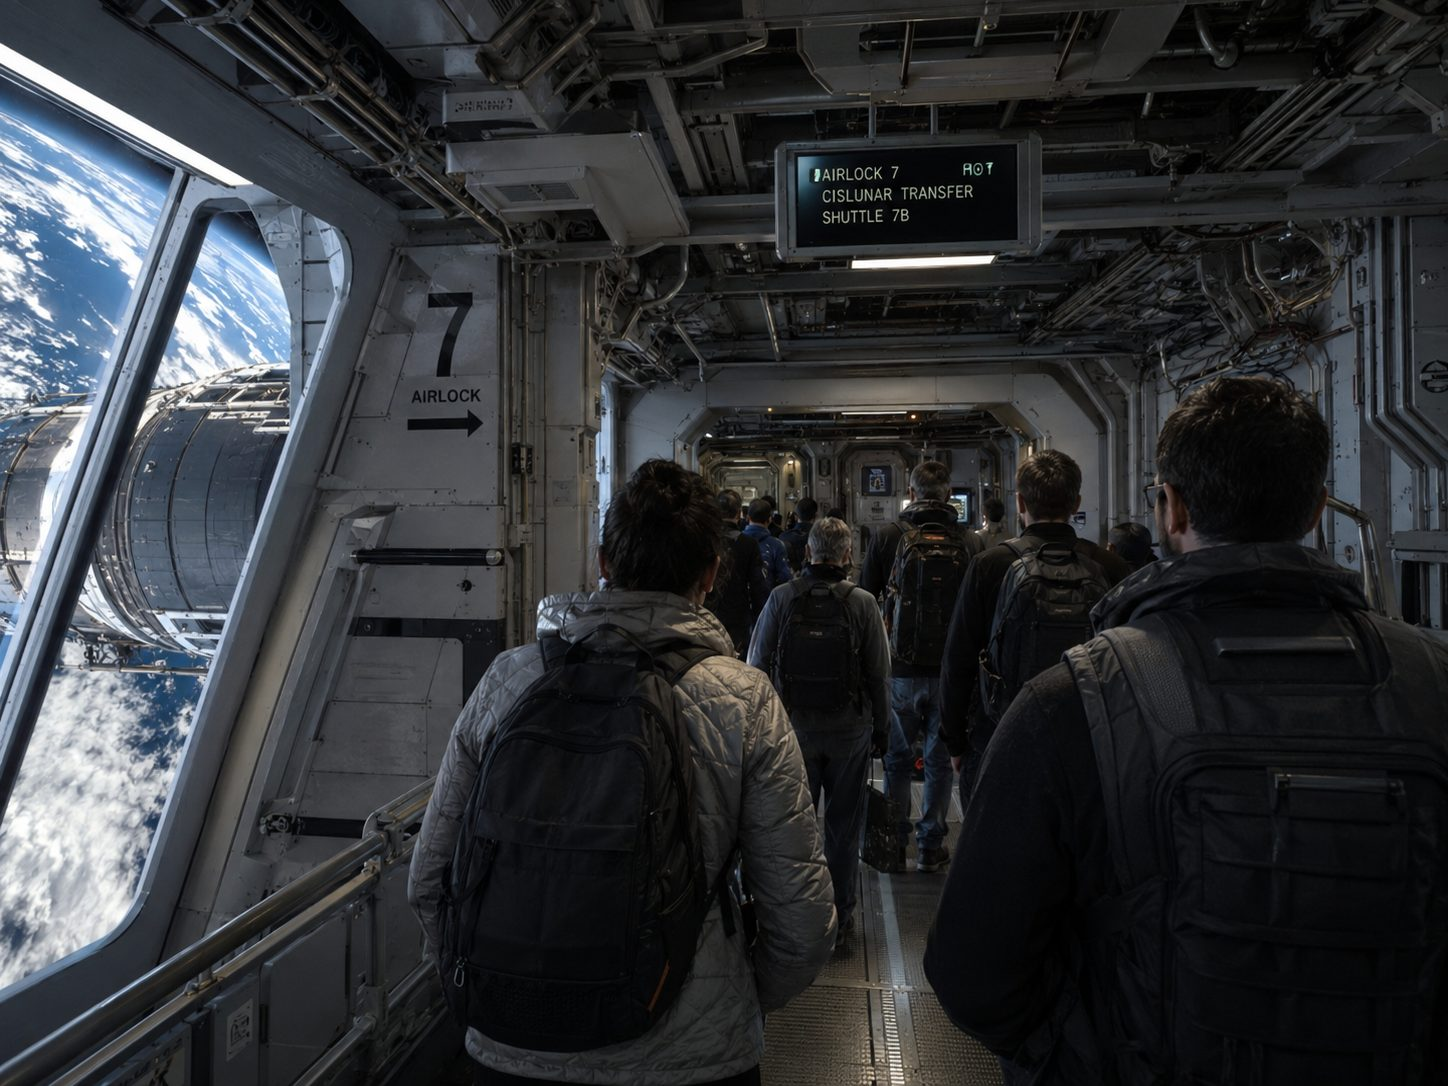
\includegraphics[width=0.9\textwidth]{00_4_pasilloindustrialhacialaesclusa7.jpg}
\end{figure}

\vspace{1.5em}
\begin{center}$\ast$\quad$\ast$\quad$\ast$\end{center}
\vspace{1.5em}

\chapter*{Acto I — El aeropuerto bajo la Tierra}
\addcontentsline{toc}{chapter}{Acto I — El aeropuerto bajo la Tierra}
\markboth{Acto I — El aeropuerto bajo la Tierra}{Acto I — El aeropuerto bajo la Tierra}

*\textit{Día 1. Lanzadera cislunar. Trayectoria LEO → Puerto Cislunar.}*

\begin{figure}[h]
\centering
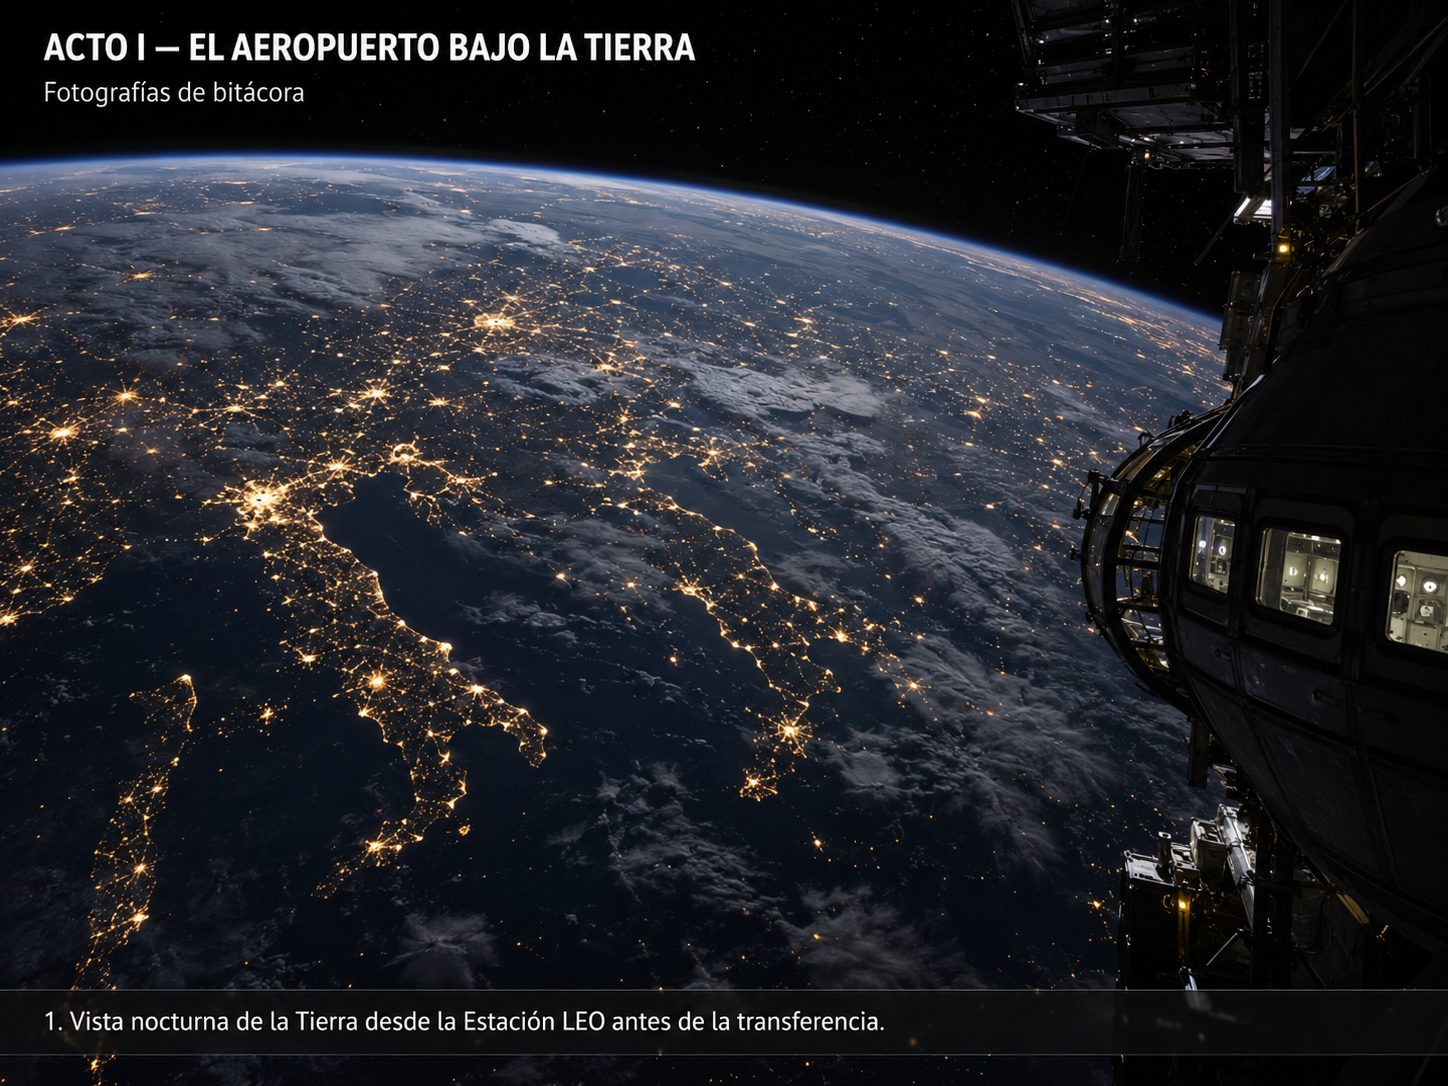
\includegraphics[width=0.9\textwidth]{01_1_vistanocturnadesdelaestacinleo.jpg}
\end{figure}

La lanzadera que nos llevó desde LEO hasta el Puerto Cislunar no parecía una nave heroica. Era fea, compacta, práctica. Una cápsula alargada con depósitos externos, radiadores plegados y un remolcador acoplado a popa.

A nadie le importaba. En el transporte espacial, la belleza había perdido la guerra contra el mantenimiento.

Nos desacoplamos de la Estación LEO durante la noche terrestre. La maniobra fue tan suave que algunos pasajeros no se dieron cuenta de que ya habíamos partido. Solo cuando la estación empezó a alejarse por las ventanillas laterales —lentamente, como un edificio que decide mudarse— alguien lo comentó en voz baja.

\begin{figure}[h]
\centering
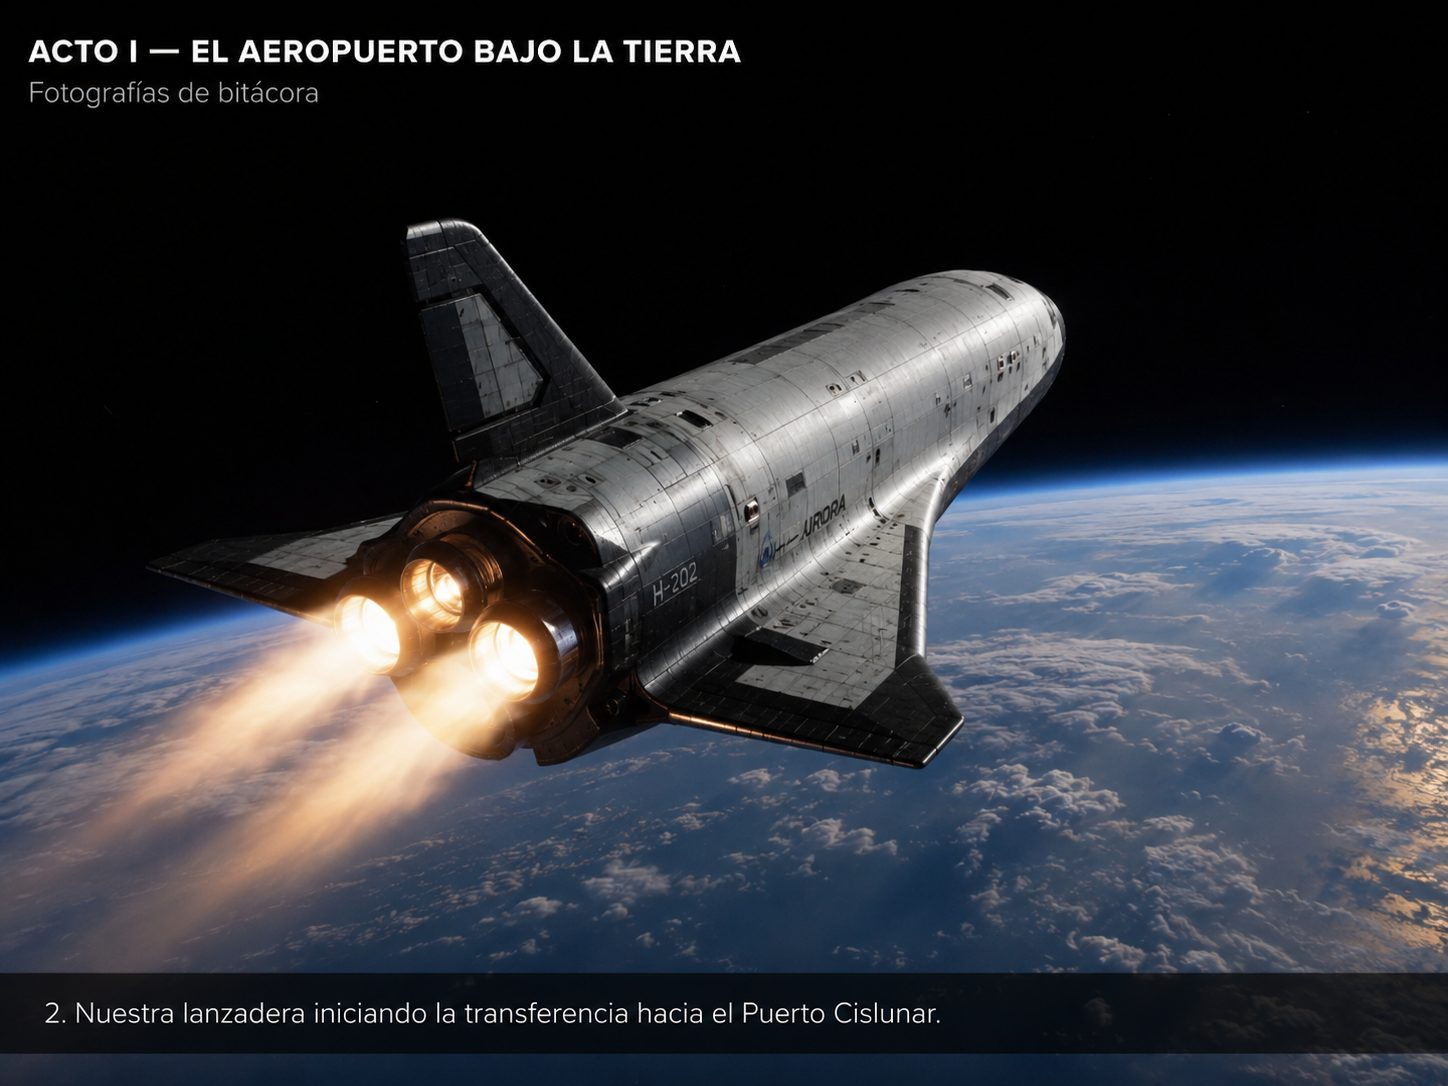
\includegraphics[width=0.9\textwidth]{01_2_lanzaderasobrelatierracislunar.jpg}
\end{figure}

En el puerto de LEO, los últimos veinte minutos antes de la salida, había podido observar la maquinaria del sistema en movimiento. Decenas de aviones orbitales entraban y salían con una precisión casi obscena. Algunos venían de plataformas ecuatoriales. Otros de pistas hipersónicas en el Pacífico. Otros eran simples cohetes reutilizables de carga, todavía necesarios, todavía ruidosos, todavía demasiado caros para el romanticismo. Cada uno de ellos había atravesado la atmósfera, había sobrevivido la reentrada o el ascenso, y ahora se acoplaba o desacoplaba con la precisión de un autobús llegando a su parada.

\begin{figure}[h]
\centering
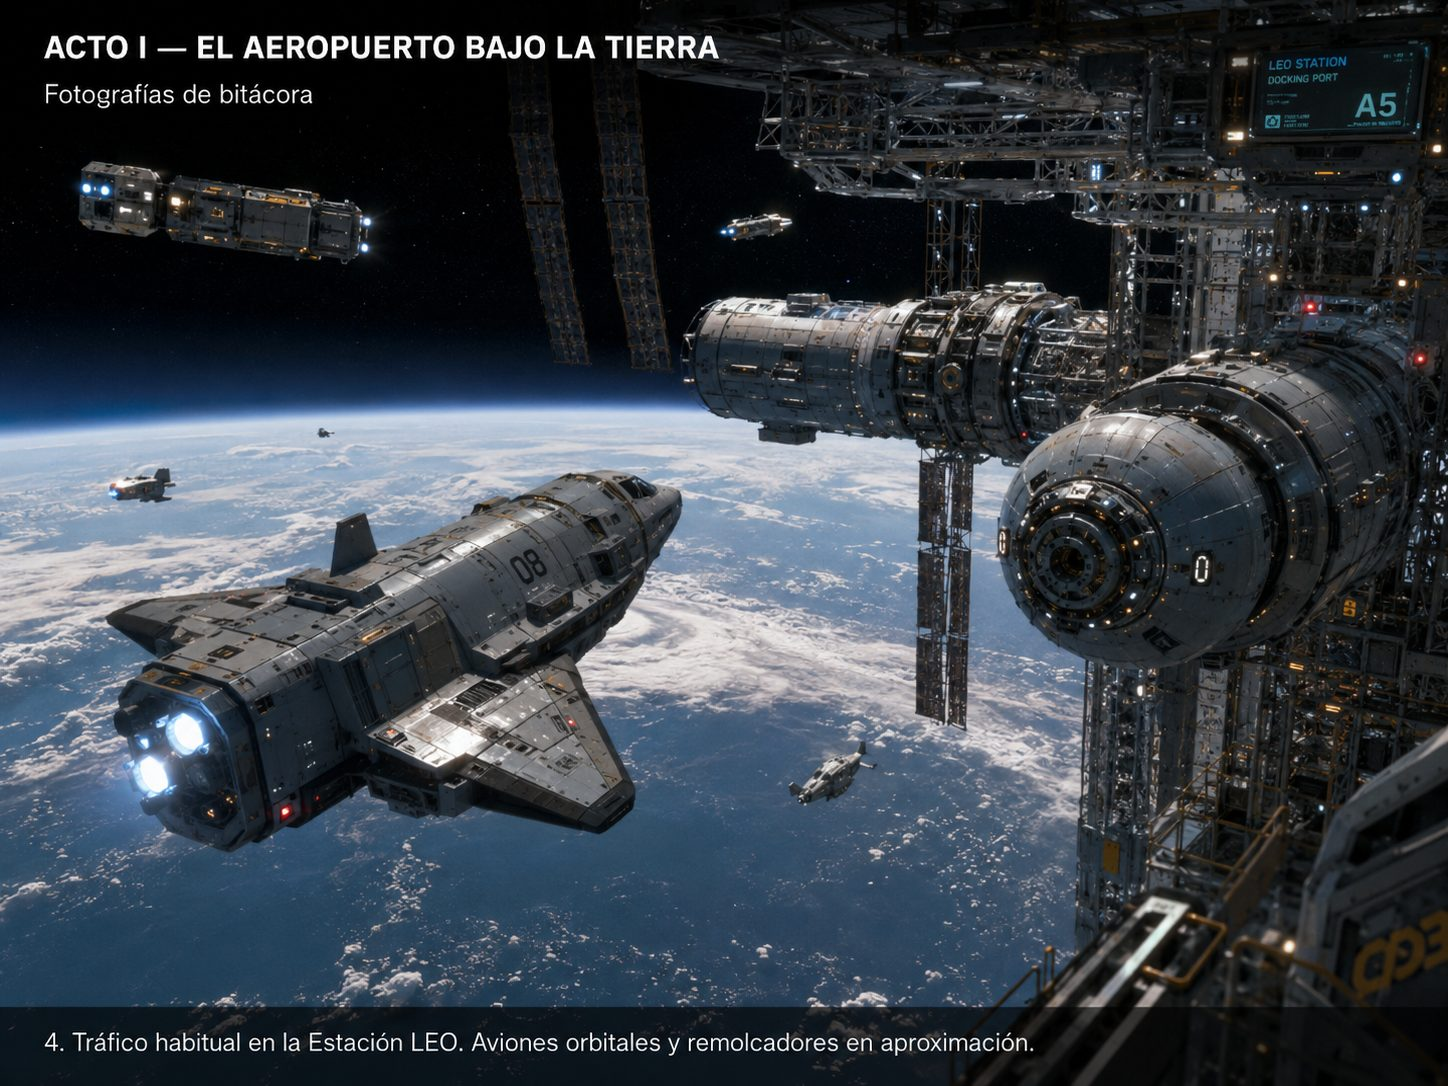
\includegraphics[width=0.9\textwidth]{01_3_trficoenlaestacinleo.jpg}
\end{figure}

Desde mi ventanilla vi un avión orbital aproximarse al vientre iluminado de la estación. Tenía el morro ennegrecido por reentradas anteriores y las alas llenas de paneles térmicos reemplazados. Las marcas de reparación lo cubrían como cicatrices de un animal que lleva años haciendo el mismo viaje. Parecía un viejo animal migratorio. Parecía exactamente lo que era.

\begin{figure}[h]
\centering
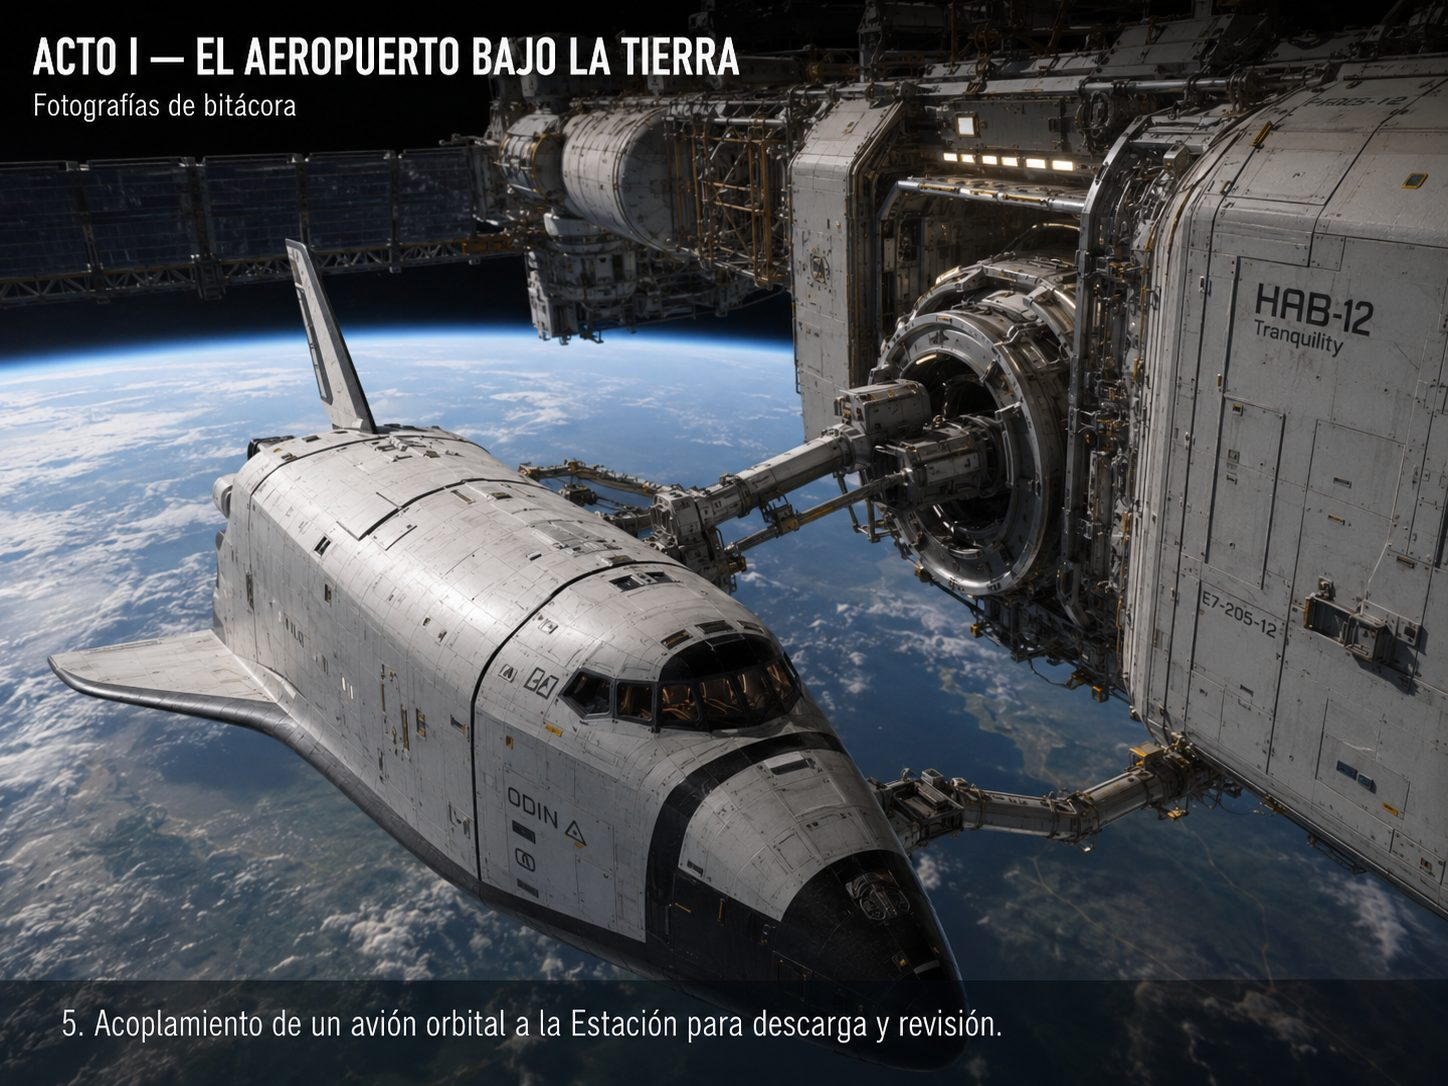
\includegraphics[width=0.9\textwidth]{01_4_acoplamientoenlaestacinespacial.jpg}
\end{figure}

Cuando encendimos motores, no hubo sacudida. Solo una presión leve en la espalda, como si el asiento hubiera tomado una decisión callada.

La Tierra empezó a hacerse pequeña.

\begin{figure}[h]
\centering
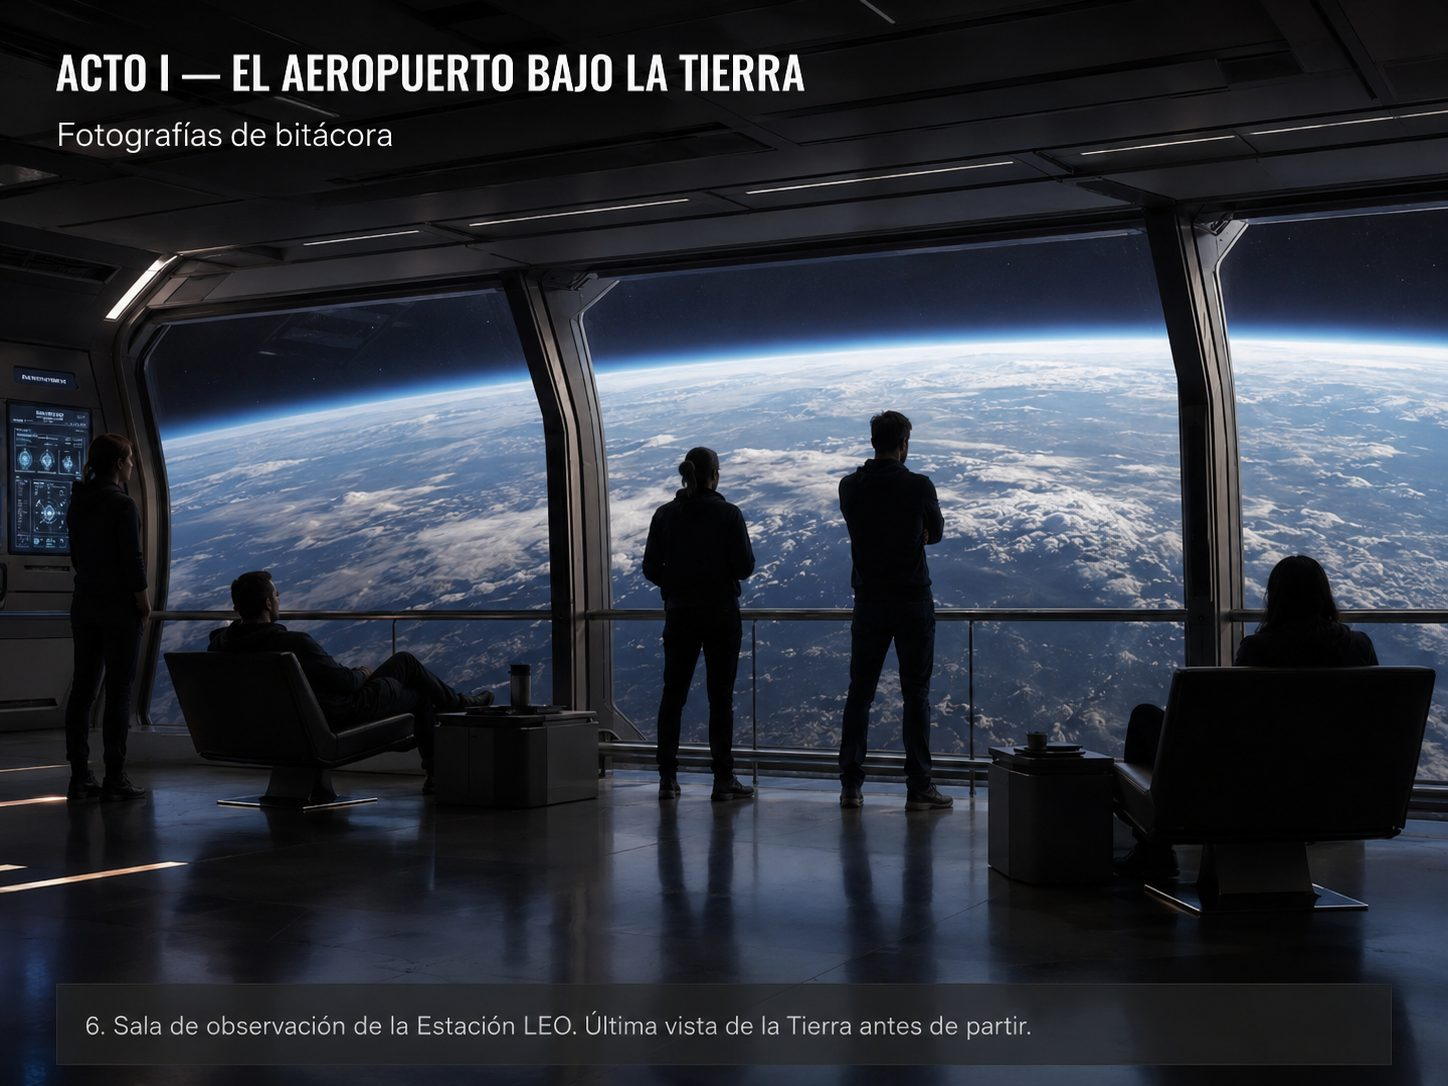
\includegraphics[width=0.9\textwidth]{01_5_ltimavistadesdelaestacinleo.jpg}
\end{figure}

El comandante habló por el canal abierto:

—Tiempo estimado al Puerto Cislunar: diecinueve horas. Trayectoria de baja energía con asistencia lunar parcial. Por favor, mantengan sellados los compartimentos privados durante la maniobra de inserción.

Nadie aplaudió. Los viajes espaciales ya no eran novedad. Pero cuando la Luna apareció por el borde de la Tierra, incluso los pasajeros frecuentes dejaron de hablar.

\begin{figure}[h]
\centering
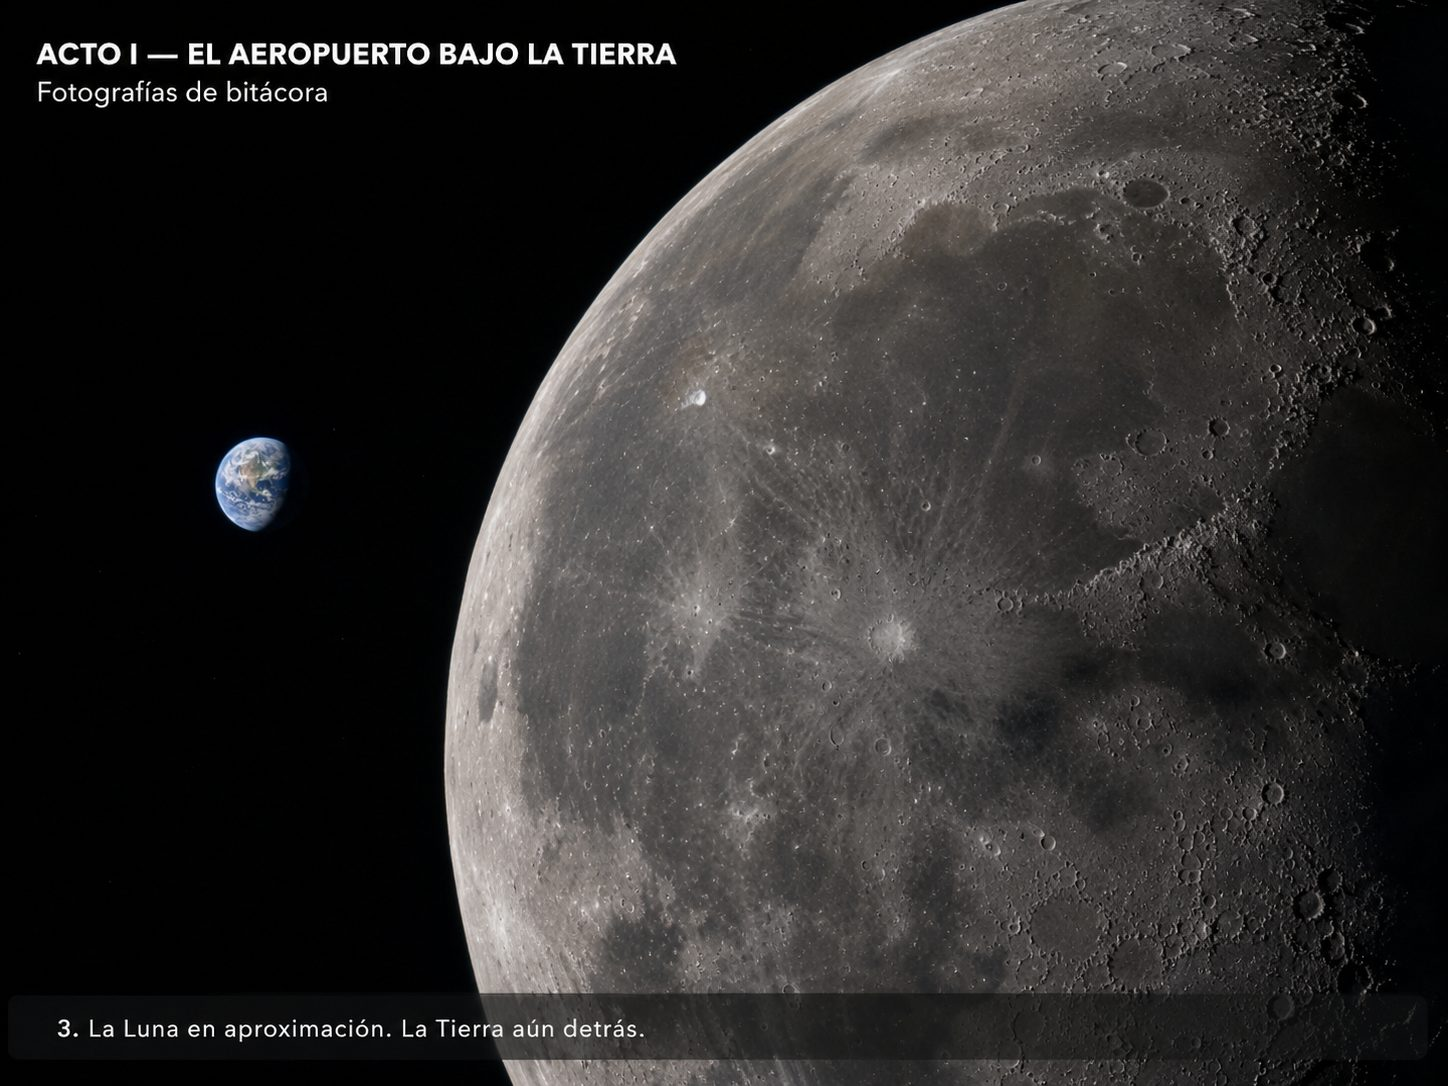
\includegraphics[width=0.9\textwidth]{01_6_lalunaenaproximacin.jpg}
\end{figure}

La Luna era gris, enorme, llena de cicatrices. Tenía cráteres que existían antes de que nuestra especie se pusiera de pie. Y alrededor de ella, como polvo metálico atrapado en una telaraña invisible, brillaban estaciones, astilleros y reflectores. Un enjambre silencioso de construcciones que ninguno de sus cráteres había visto venir.

Pasé gran parte del trayecto mirando esa luna envuelta en metal. Las diecinueve horas me parecieron muy cortas.

La primera vez que vi el *\textit{Puerto Cislunar}* en los sensores —primero como un conjunto de puntos de calor, luego como estructuras distinguibles en la pantalla de navegación, finalmente como una presencia que ocupaba la ventanilla completa— pensé que la humanidad había construido una ciudad donde no debía haber nada.

Luego pensé que ese era exactamente su estilo.

\vspace{1.5em}
\begin{center}$\ast$\quad$\ast$\quad$\ast$\end{center}
\vspace{1.5em}

\chapter*{Acto II — Puerto Cislunar}
\addcontentsline{toc}{chapter}{Acto II — Puerto Cislunar}
\markboth{Acto II — Puerto Cislunar}{Acto II — Puerto Cislunar}

*\textit{Días 2–4. Puerto Cislunar. Órbita halo L1/L2 Tierra-Luna.}*

El Puerto Cislunar no era una estación. Era una región habitada.

\begin{figure}[h]
\centering
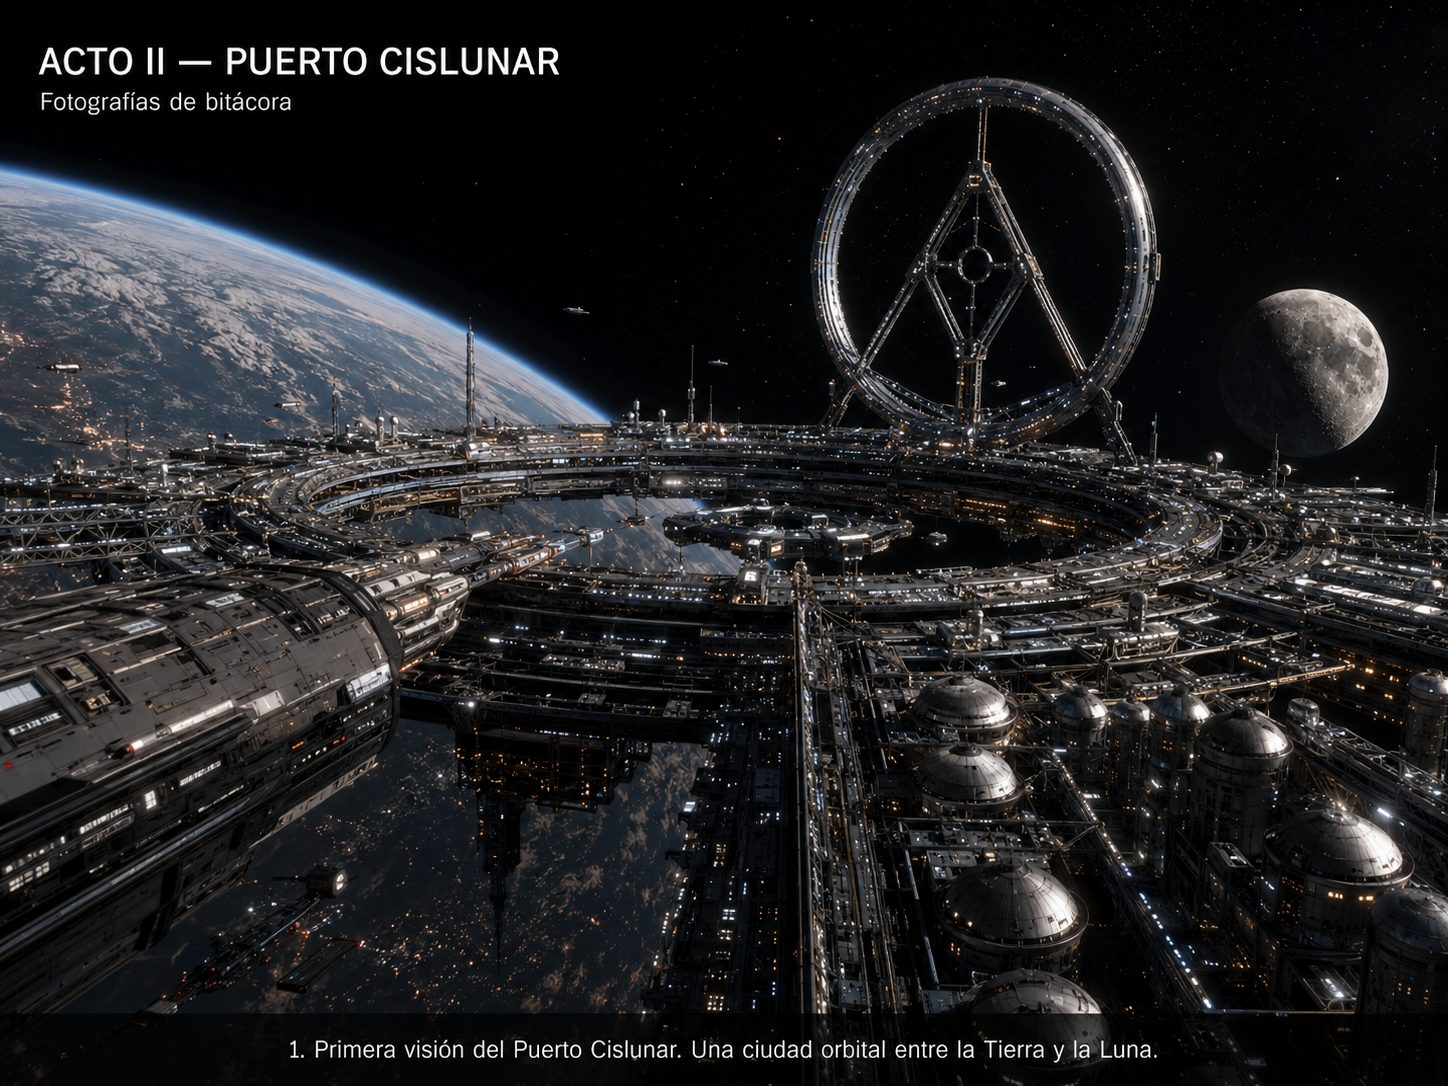
\includegraphics[width=0.9\textwidth]{02_1_puertocislunarentrelatierraylaluna.jpg}
\end{figure}

Eso tardé dos horas en entenderlo, después de acodarme junto a la ventana panorámica del pasillo de llegadas y ver que lo que tenía delante no cabía en ningún encuadre. El núcleo principal flotaba en una órbita halo, lejos de la Tierra y lo bastante cerca de la Luna como para alimentarse de sus astilleros. Desde allí dentro, si te asomabas al ángulo correcto, podías ver la Tierra y la Luna al mismo tiempo, colgando cada una en su parte del cielo negro.

Se distinguían tres estructuras principales: el anillo civil, los muelles convencionales y la *\textit{catapulta geométrica interior}*.

La catapulta era lo más extraño.

No parecía un portal. No había una superficie líquida ni un remolino brillante. Era un anillo incompleto de kilómetros de diámetro, formado por segmentos separados, radiadores y enormes bobinas de campo. Tenía la frialdad estética de algo diseñado por ingenieros que no necesitaban convencer a nadie. En su interior, una nave pequeña esperaba suspendida entre haces de alineación azulada, perfectamente quieta, como una bala que ya sabe adónde va.

\begin{figure}[h]
\centering
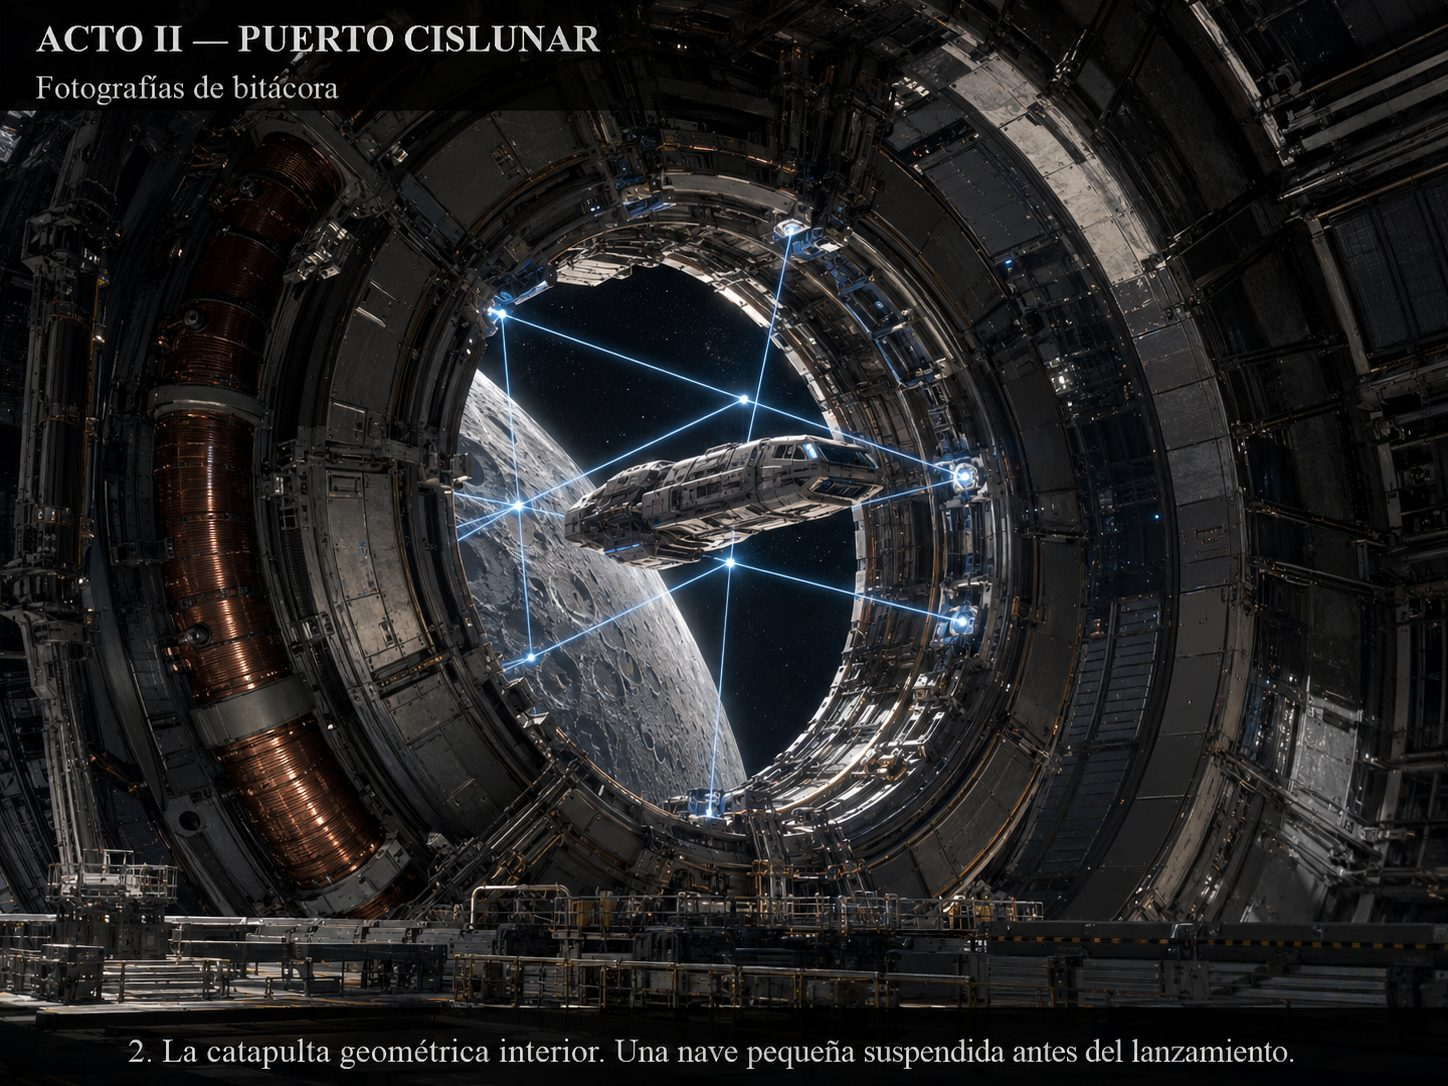
\includegraphics[width=0.9\textwidth]{02_2_lanzamientoenelpuertocislunar.jpg}
\end{figure}

La guía del puerto nos lo explicó durante el acoplamiento con la eficiencia de quien lleva años diciendo lo mismo sin aburrirse:

—Las naves pequeñas no llevan motor warp completo. Pesaría más que la propia nave. El puerto genera la burbuja inicial, la estabiliza y la inyecta en un corredor certificado. La nave solo mantiene el campo residual hasta el nodo de destino.

—¿Y si falla? —preguntó alguien.

La guía no sonrió.

—Entonces no se lanza.

Me gustó aquella respuesta. Era seca, honesta, humana.

Pasé tres días en el Puerto Cislunar. Tenía tiempo antes de que saliera el Kepler-Sancho y decidí usarlo para mirar. Allí convivían tres épocas del transporte espacial con la naturalidad de quien no ve el problema.

En un muelle vi cargueros de fusión lenta cargando agua lunar hacia Marte, exactamente como los barcos de vapor cargaban carbón hace tres siglos.

\begin{figure}[h]
\centering
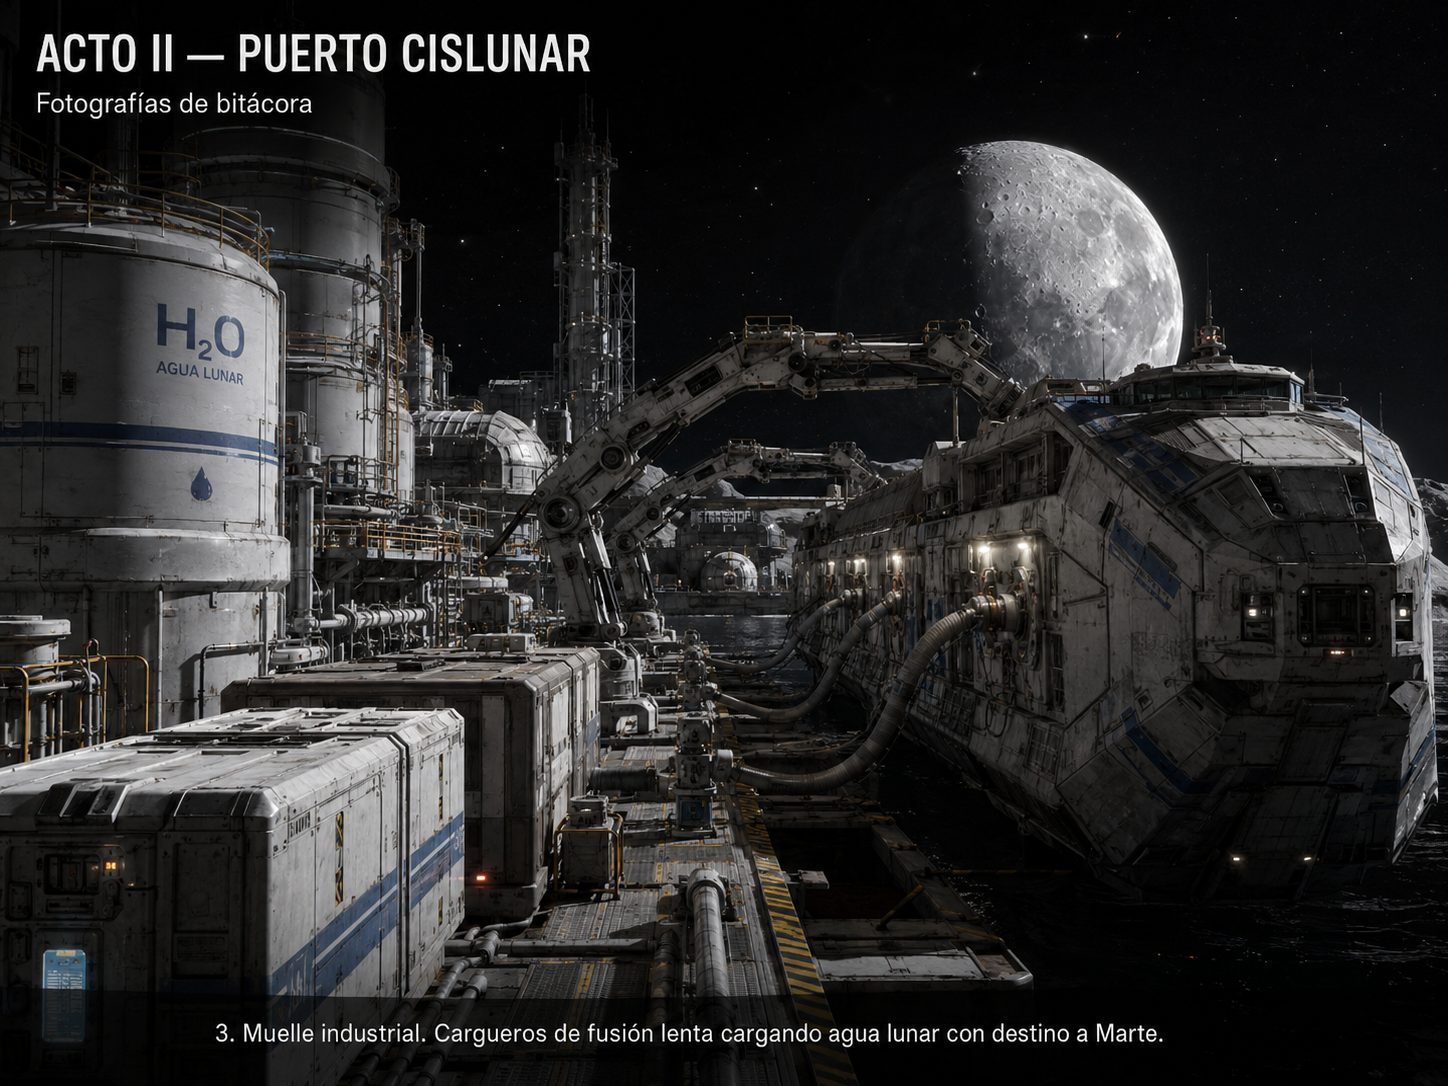
\includegraphics[width=0.9\textwidth]{02_3_puertoindustrialcislunarendetalle.jpg}
\end{figure}

En otro, un cicler clásico preparaba su ruta a Ceres, con pasajeros de bajo presupuesto y toneladas de maquinaria agrícola durmiendo en la bodega. El cicler olía a aceite y a muchas reparaciones. Era glorioso a su manera.

\begin{figure}[h]
\centering
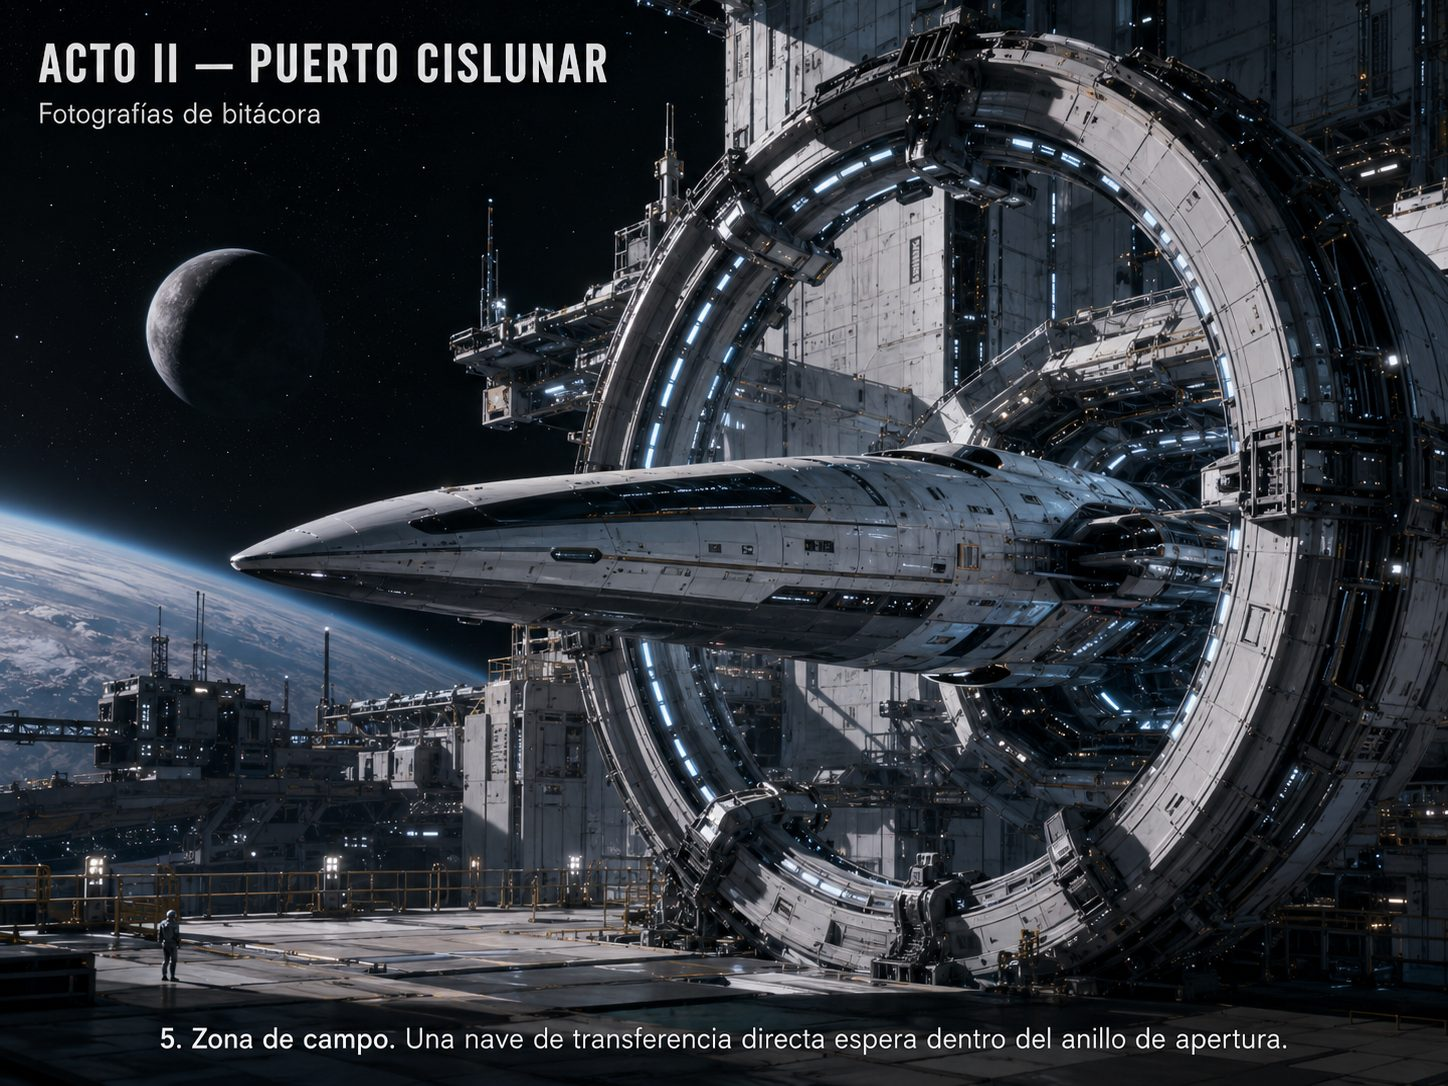
\includegraphics[width=0.9\textwidth]{02_4_puertocislunaresperadetransferencia.jpg}
\end{figure}

Más allá, en la zona de campo, una nave de transferencia directa esperaba dentro del anillo de apertura. Una bala dentro de un cañón construido por arquitectos pacientes.

\begin{figure}[h]
\centering
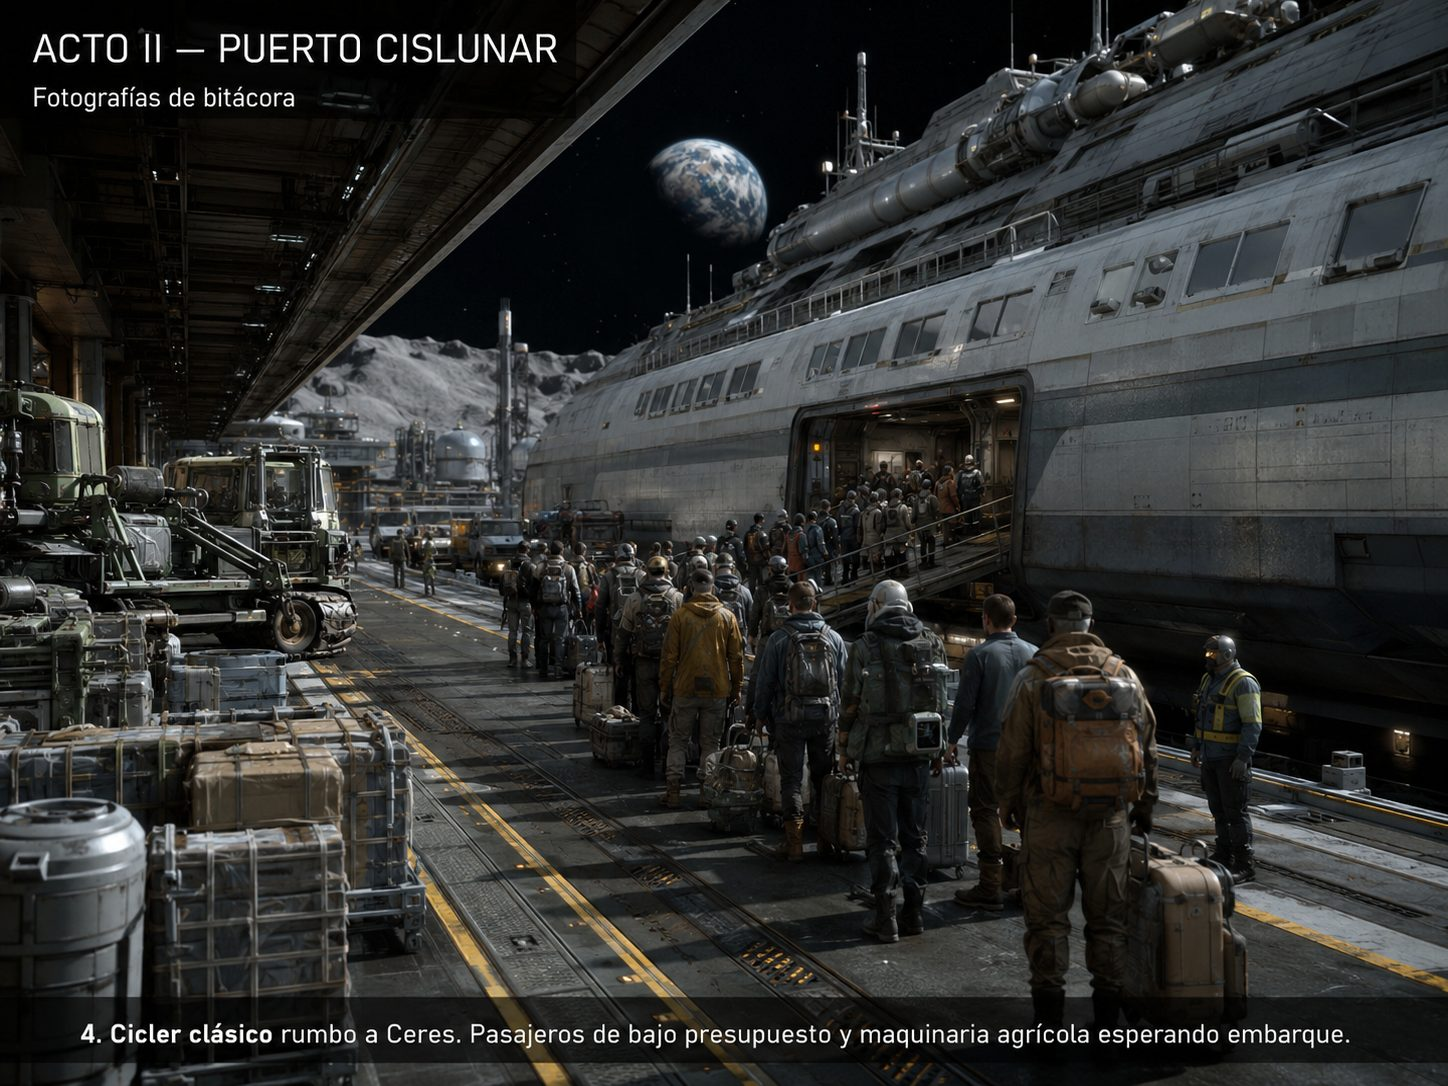
\includegraphics[width=0.9\textwidth]{02_5_puertoespacialenlaluna.jpg}
\end{figure}

El puerto olía a metal filtrado, aire reciclado y comida demasiado especiada. En los corredores civiles había niños lunares corriendo con pasos largos y torpes: habían crecido en 0,16g y sus cuerpos no sabían del todo cómo comportarse en gravedad más alta. Corrían como si el suelo fuera una sugerencia. En las ventanas panorámicas, turistas terrestres lloraban en silencio al ver la Tierra suspendida sobre el negro. Una mujer tenía la mano apoyada en el cristal.

No le hice una foto. Algunas cosas no mejoran con ser fotografiadas.

El tercer día embarqué en el *\textit{Cicler de Campo Kepler-Sancho}*, línea regular Cislunar-Fobos-Ceres.

\begin{figure}[h]
\centering
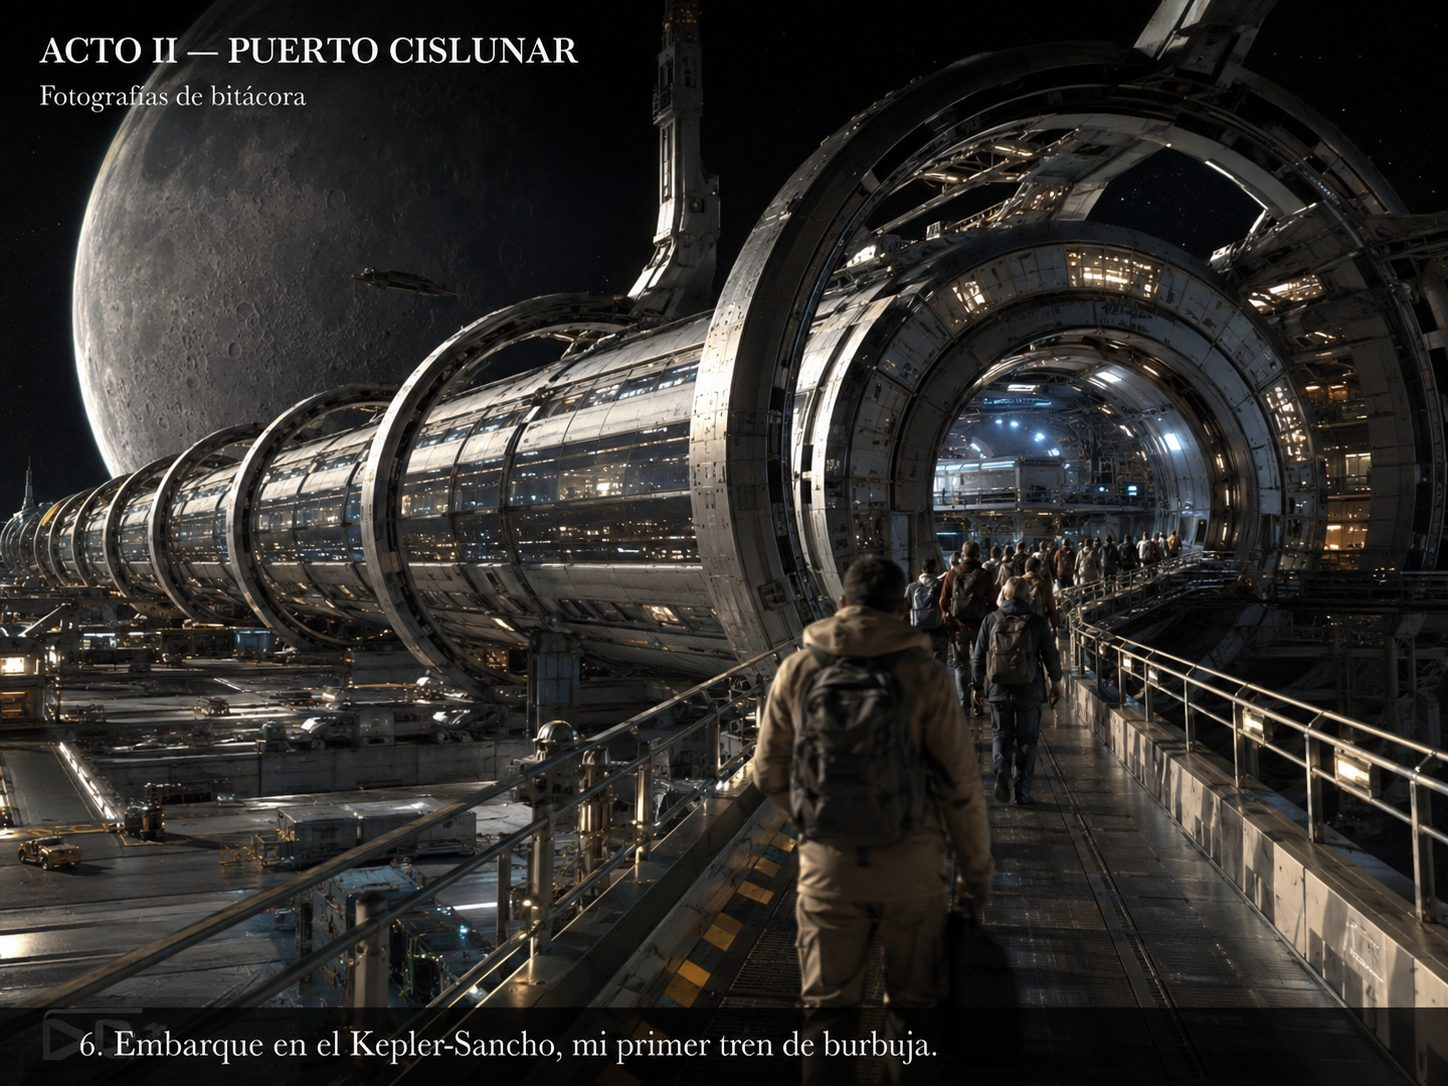
\includegraphics[width=0.9\textwidth]{02_6_embarquehaciaelkeplersancho.jpg}
\end{figure}

Era mi primer tren de burbuja. Fui el último en subir. Me quedé parado en la esclusa de embarque un momento, mirando hacia atrás, hacia el anillo civil del Puerto Cislunar. Luego cerré la esclusa.

\vspace{1.5em}
\begin{center}$\ast$\quad$\ast$\quad$\ast$\end{center}
\vspace{1.5em}

\chapter*{Acto III — El tren hacia Marte}
\addcontentsline{toc}{chapter}{Acto III — El tren hacia Marte}
\markboth{Acto III — El tren hacia Marte}{Acto III — El tren hacia Marte}

*\textit{Días 5–7. Cicler de Campo Kepler-Sancho. Corredor Cislunar-Fobos Tres.}*

El Kepler-Sancho tenía casi tres kilómetros de longitud.

\begin{figure}[h]
\centering
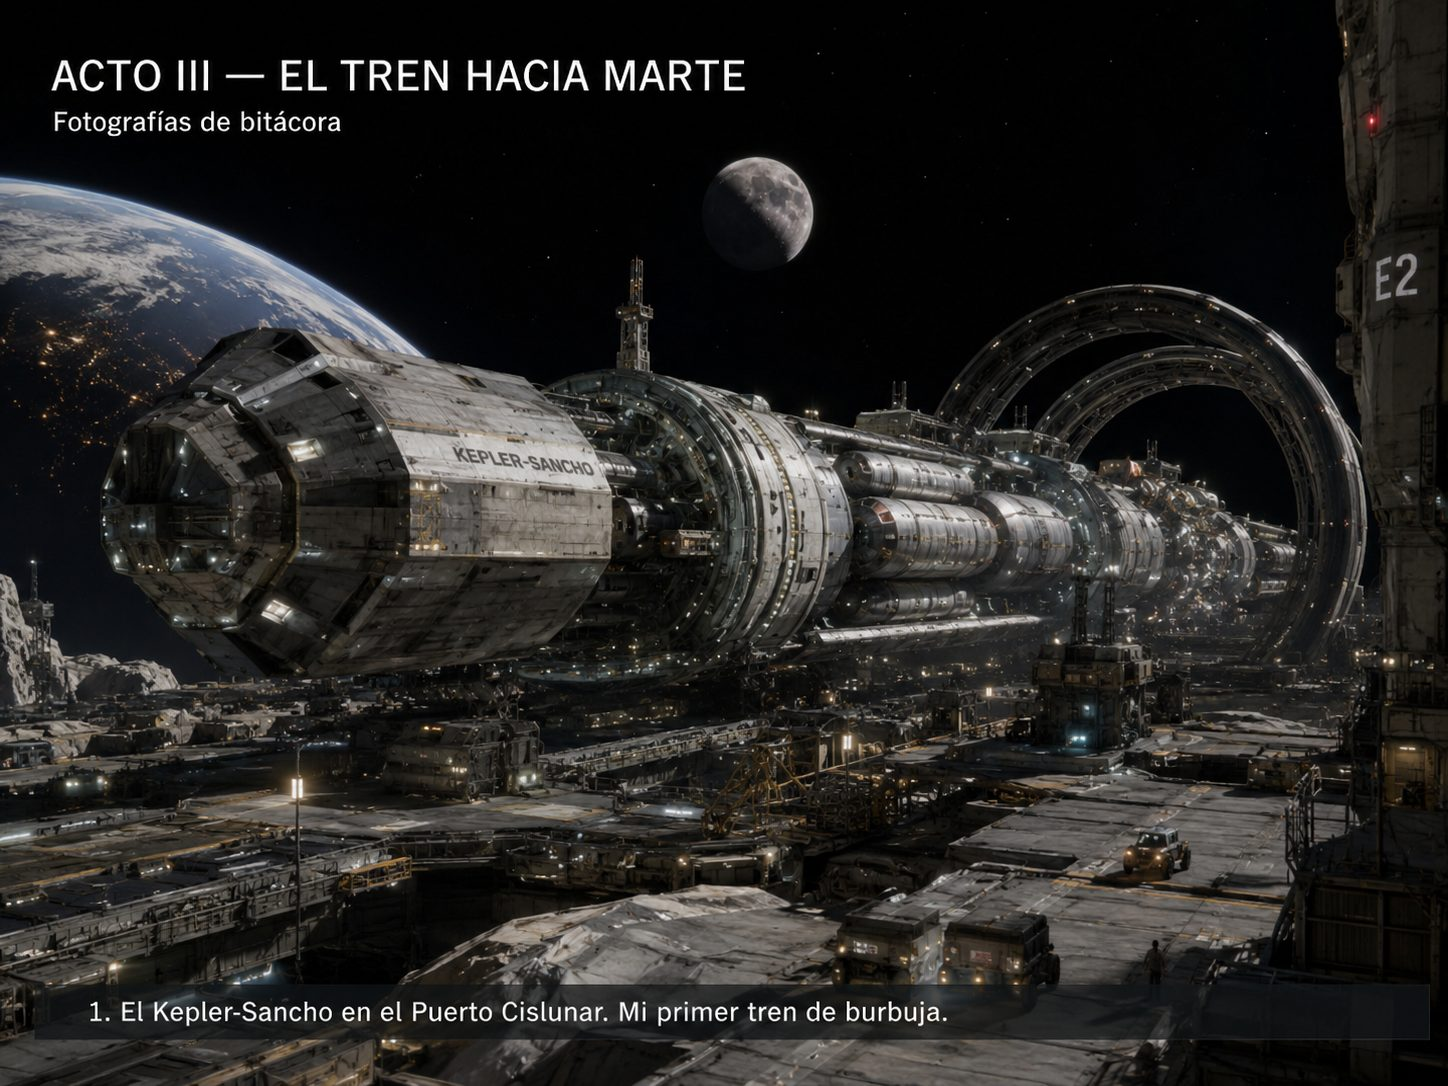
\includegraphics[width=0.9\textwidth]{03_1_elkeplersanchoenelpuertocislunar.jpg}
\end{figure}

La primera vez que lo vi completo, desde un muelle exterior del Puerto Cislunar, tardé varios segundos en procesar que era un único objeto. Cabezas de la cola que no podía ver desde donde estaba. Estructuras que conectaban tramos con tramos. Una nave que parecía un pueblo.

Su sección delantera era un escudo: capas de hielo, cerámica, campos magnéticos y drones de barrido que trabajaban en turnos continuos. Detrás venían los hábitats giratorios, dos anillos lentos donde la gravedad simulada alcanzaba 0,6g. Más atrás, contenedores, talleres, depósitos y, al final, los anillos de curvatura. Tenía la elegancia de las cosas que no intentan ser elegantes.

No era un avión espacial. Era un tren. Era exactamente eso.

Antes de la salida, nos reunieron en la sala de observación principal. El capitán, una mujer marciana nacida en Fobos, apareció en las pantallas con la calma de quien lleva décadas haciendo esta misma charla:

\begin{figure}[h]
\centering
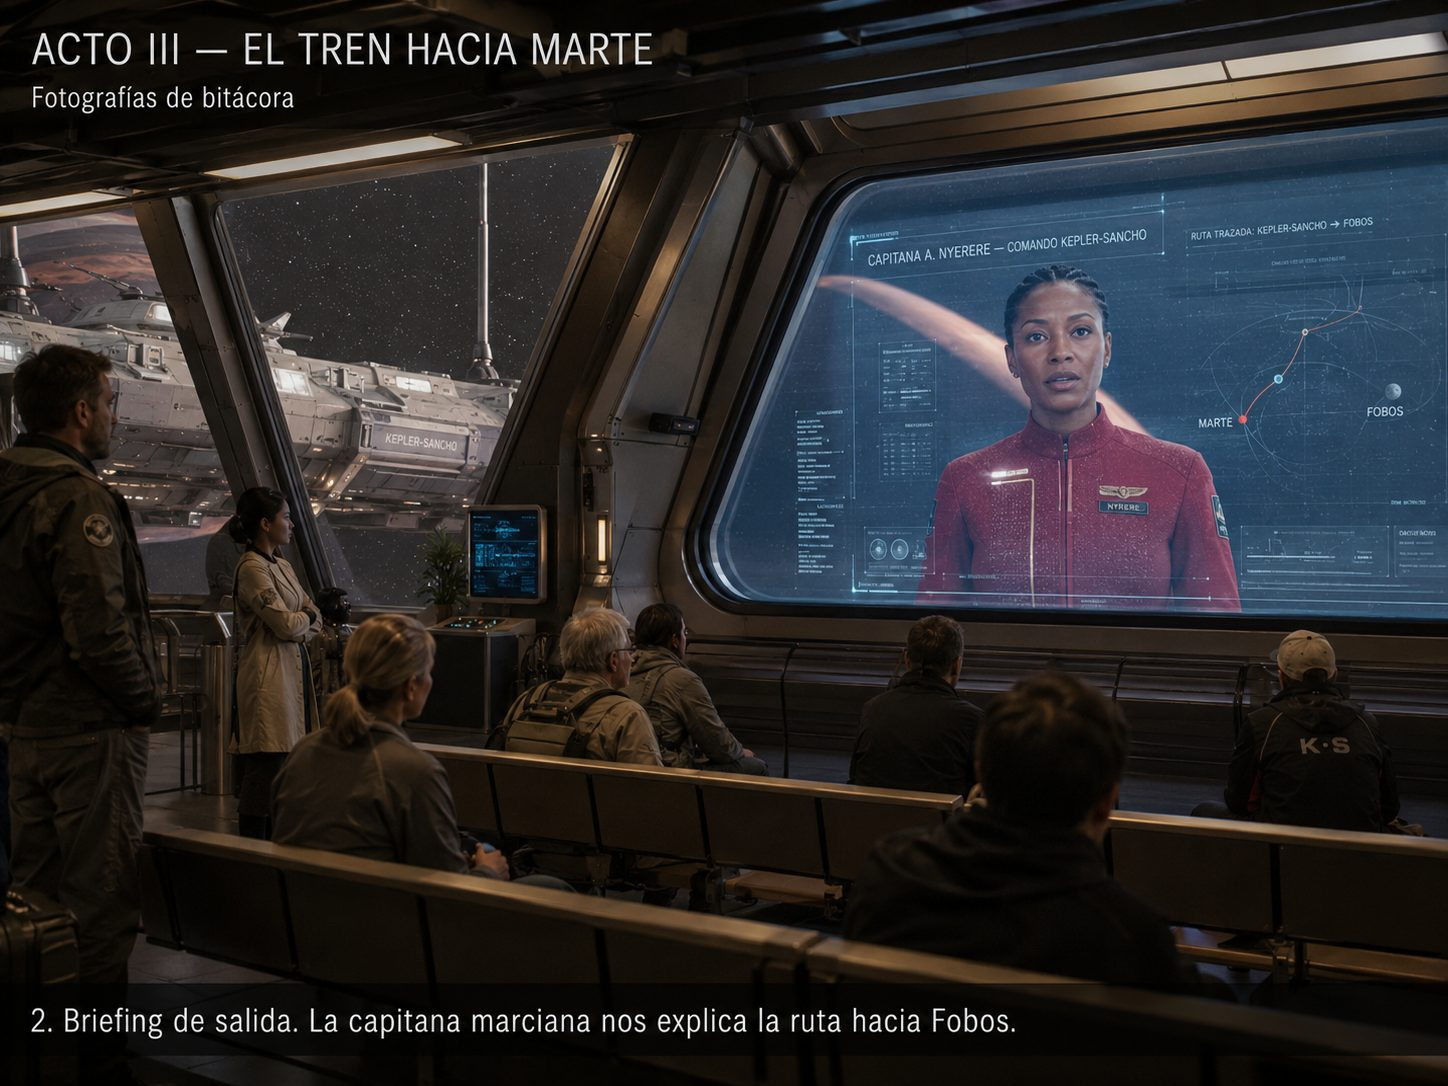
\includegraphics[width=0.9\textwidth]{03_2_briefingenlanavekeplersancho.jpg}
\end{figure}

—Vamos a usar el corredor Cislunar-Fobos Tres. Duración estimada: cuarenta y seis horas. Entraremos en campo sublumínico a 0,037c. No hay dilatación temporal significativa. No hay maniobra manual. No hay ventanas exteriores abiertas durante la fase de inserción.

Una niña preguntó si veríamos las estrellas moverse.

El capitán tardó medio segundo en responder.

—No como en las películas.

Y tenía razón.

Cuando el campo se activó, el universo no se convirtió en líneas. No hubo túnel de luz. No hubo golpe dramático ni cuenta atrás en los altavoces. Hubo un leve oscurecimiento de las estrellas delante de la nave, como si alguien hubiera tensado una membrana invisible entre nosotros y el espacio. Nada más. Los pasajeros miraron por las ventanas durante diez segundos y luego volvieron a lo que estaban haciendo.

\begin{figure}[h]
\centering
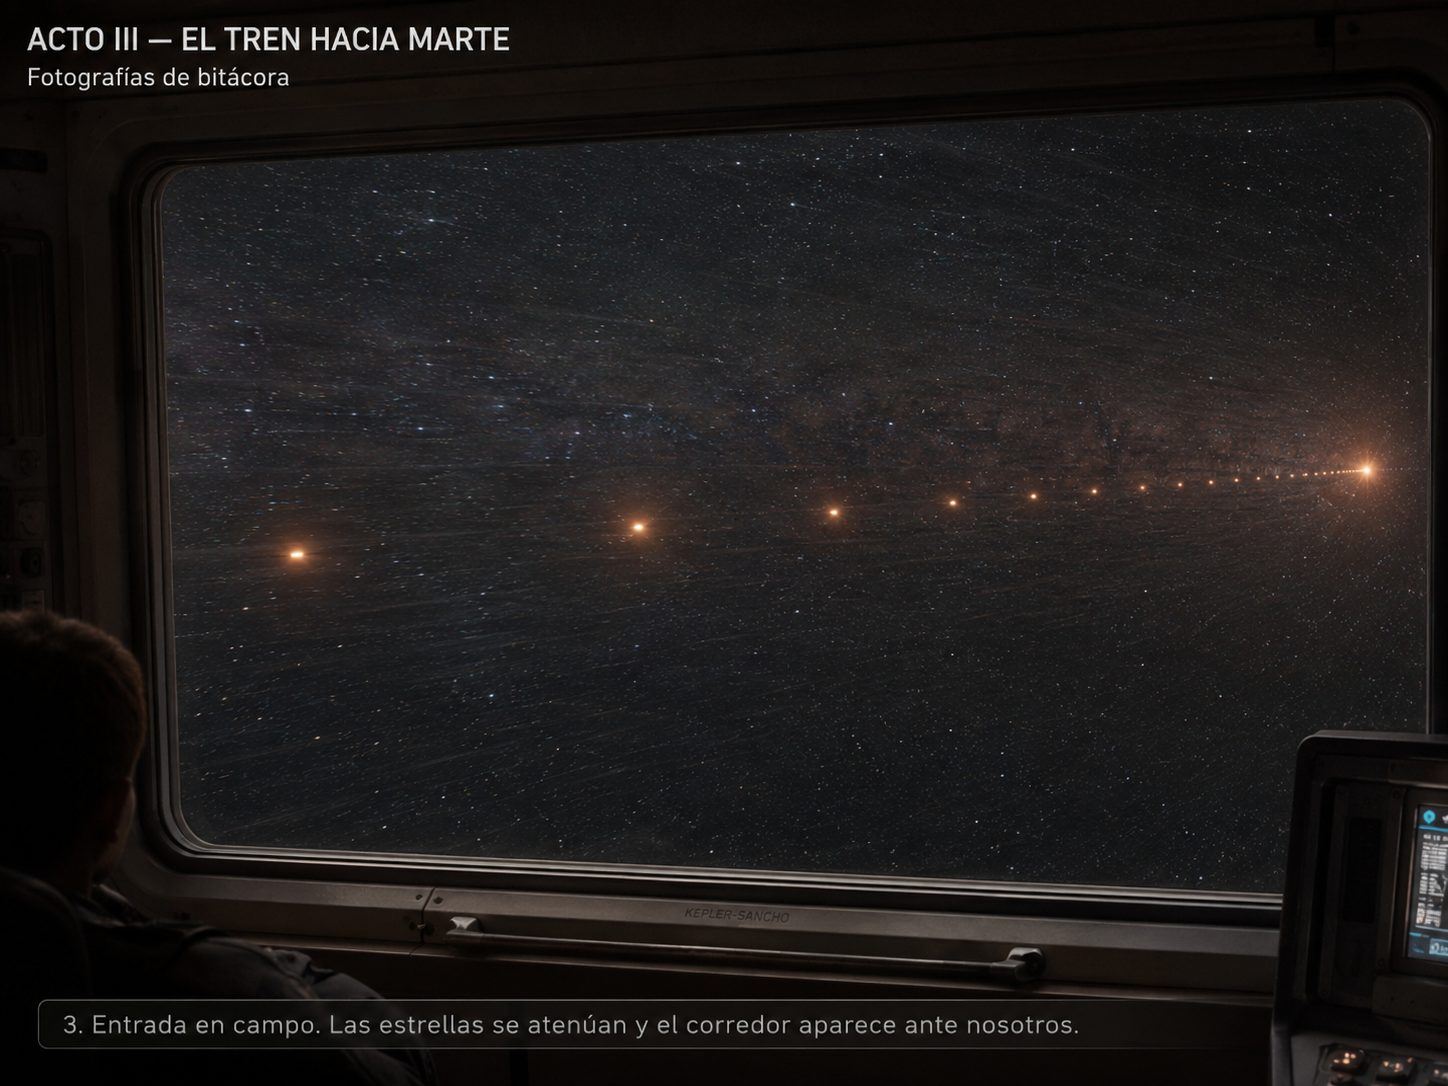
\includegraphics[width=0.9\textwidth]{03_3_actoiiieltrenhaciamarte.jpg}
\end{figure}

El corredor aparecía en los sensores como una red de balizas distribuidas a millones de kilómetros. Desde la cubierta de observación se veían algunas: puntos anaranjados, perfectamente alineados, marcando una carretera que no existía en ningún mapa físico pero que estaba allí, certificada, barrida, sostenida por drones de mantenimiento que nadie mencionaba jamás en los comunicados oficiales.

Durante el primer día, la Tierra quedó atrás. La Luna se redujo a una moneda. Marte apareció al frente, primero como una estrella roja, luego como un disco que crecía muy despacio, con la paciencia de algo que sabe que al final te llegará.

\begin{figure}[h]
\centering
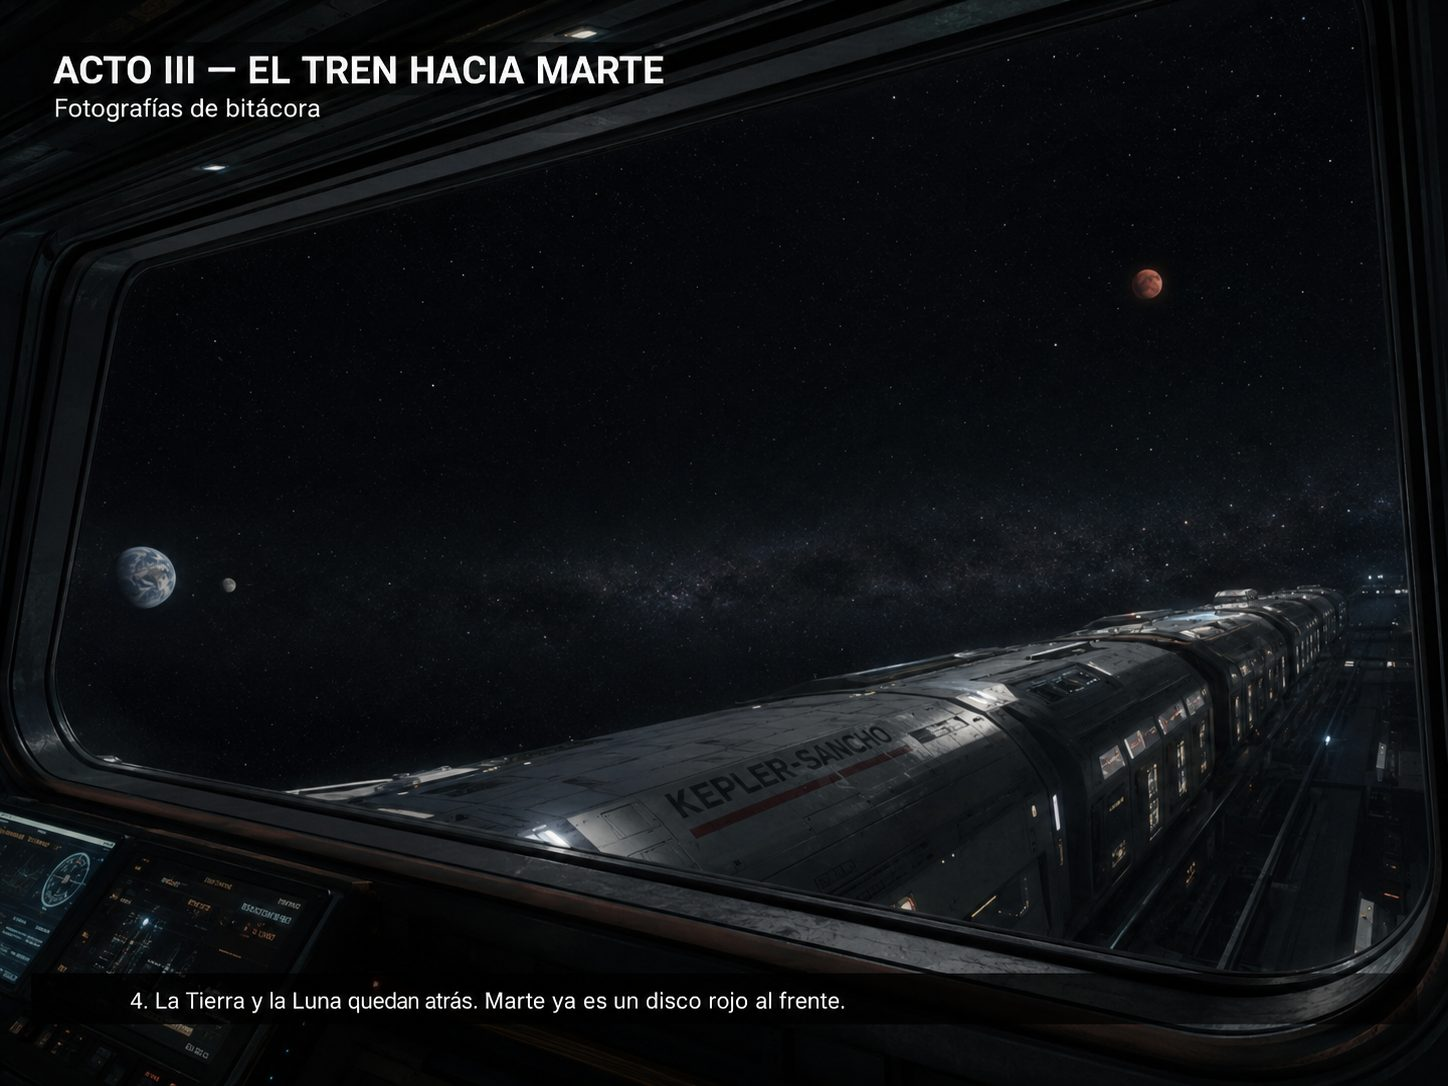
\includegraphics[width=0.9\textwidth]{03_4_viajandohaciamarteenelkeplersancho.jpg}
\end{figure}

La gente se acostumbró demasiado pronto.

Eso fue lo que más me impresionó. Al cabo de diez horas, algunos pasajeros estaban viendo series, discutiendo por turnos de ducha o quejándose del café. Alguien había organizado una partida de ajedrez. Dos adolescentes dormían en postura imposible sobre un sofá de la zona común. La humanidad podía convertir cualquier milagro en transporte público.

\begin{figure}[h]
\centering
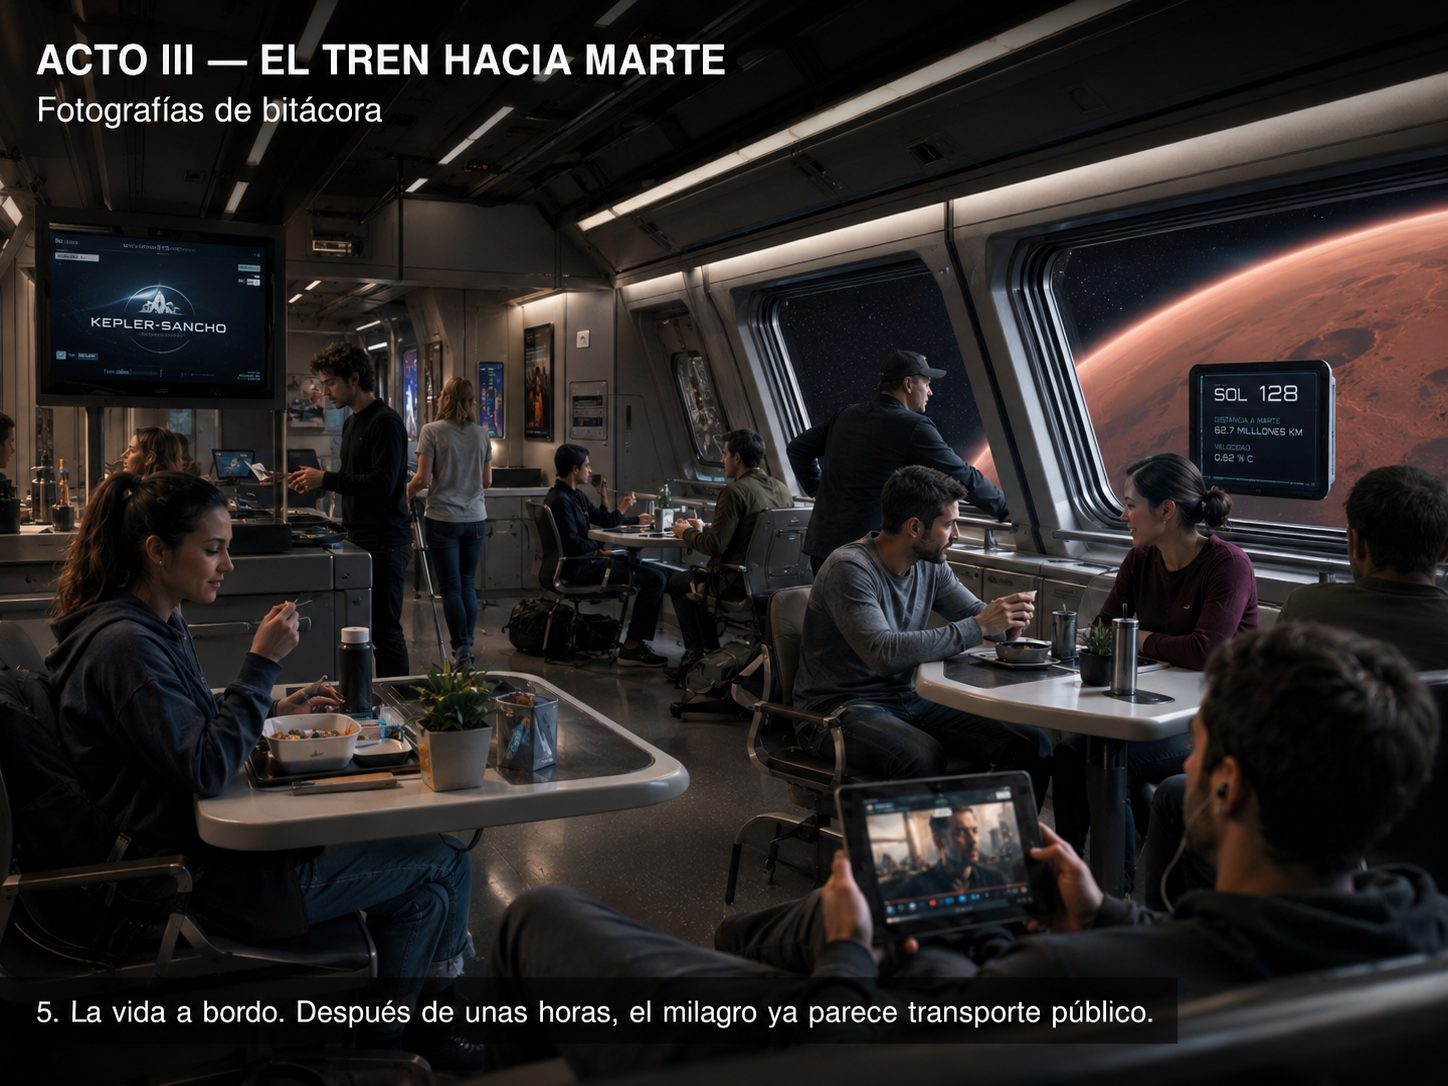
\includegraphics[width=0.9\textwidth]{03_5_lavidaeneltrenhaciamarte.jpg}
\end{figure}

Yo no pude.

Me quedé mirando Marte hasta que me dolieron los ojos. Hasta que el planeta dejó de ser una mancha roja y empezó a tener textura: nubes finísimas, irregularidades en la superficie, el hemisferio iluminado y el oscuro con el borde perfectamente nítido porque allí no había atmósfera densa que difuminara el límite.

\begin{figure}[h]
\centering
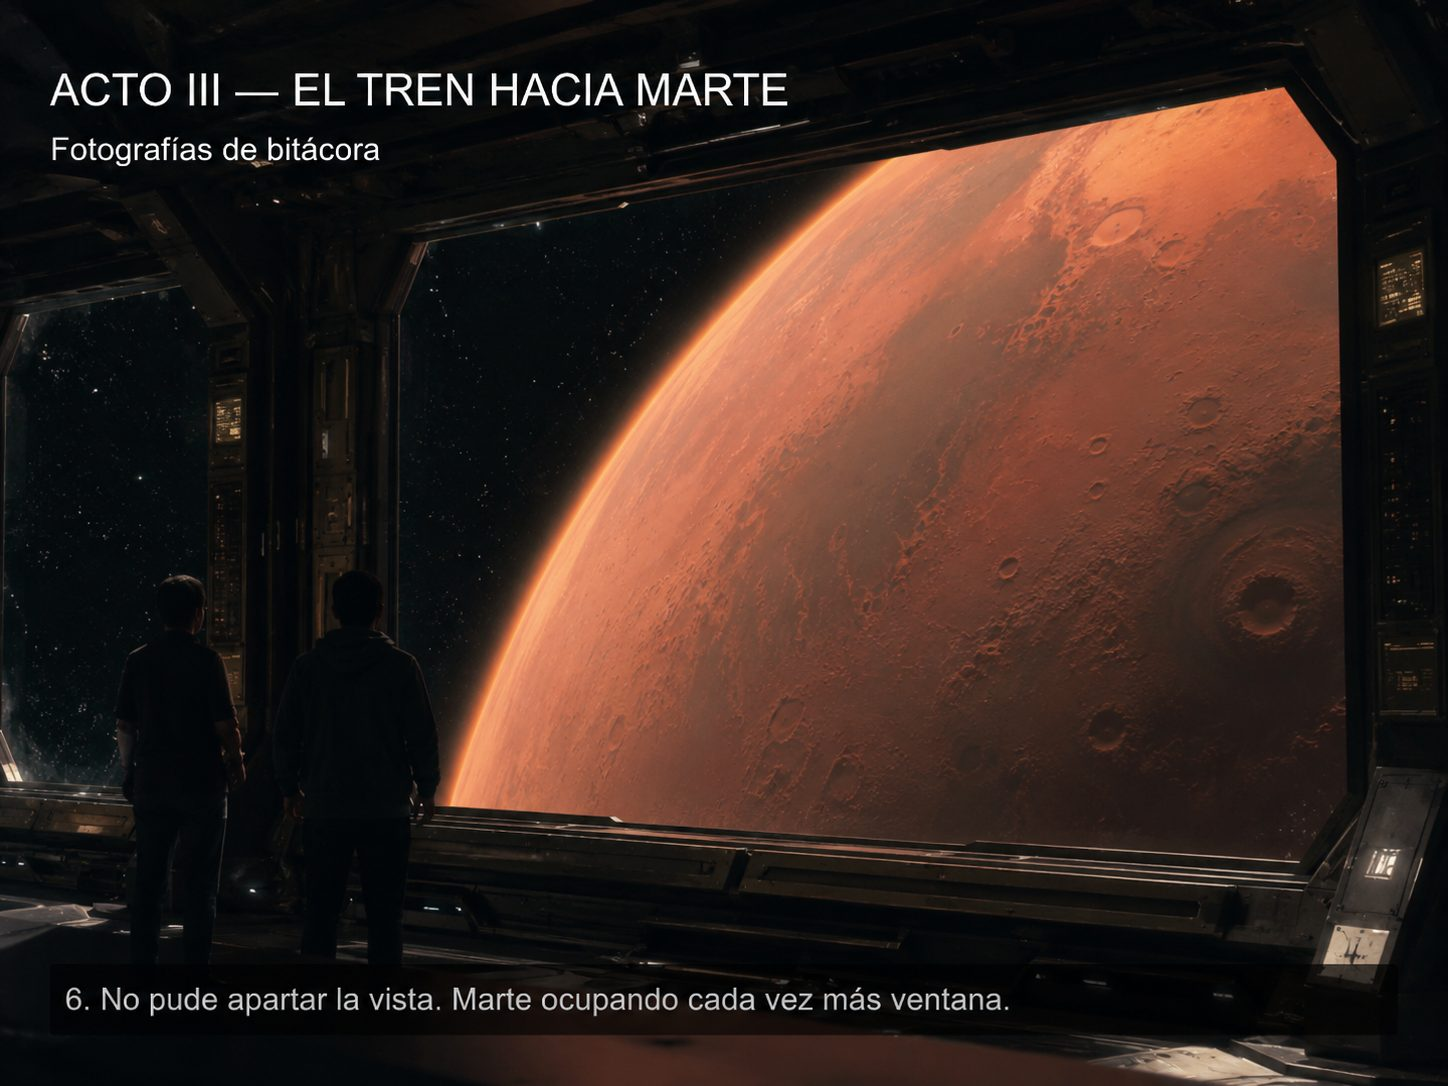
\includegraphics[width=0.9\textwidth]{03_6_miradahaciamartedesdelaestacin.jpg}
\end{figure}

En mi diario escribí:

> A 0,037c, mirando un planeta rojo crecer, pensé que los milagros no desaparecen porque te acostumbres a ellos. Solo te acostumbras a no verlos.

\vspace{1.5em}
\begin{center}$\ast$\quad$\ast$\quad$\ast$\end{center}
\vspace{1.5em}

\chapter*{Acto IV — Fobos, la luna retenida}
\addcontentsline{toc}{chapter}{Acto IV — Fobos, la luna retenida}
\markboth{Acto IV — Fobos, la luna retenida}{Acto IV — Fobos, la luna retenida}

*\textit{Días 8–12. Estación Fobos. Órbita baja marciana. Superficie de Pavonis, Marte.}*

Fobos parecía un error geológico.

Un pedrusco oscuro, irregular, demasiado cerca de Marte para tener aspecto de luna. Cuando nos aproximamos, el planeta llenaba media ventana: rojo, inmenso, con nubes finas y tormentas de polvo extendiéndose como heridas que cicatrizaban demasiado despacio. Fobos flotaba delante de ese fondo como algo que alguien había olvidado recoger.

\begin{figure}[h]
\centering
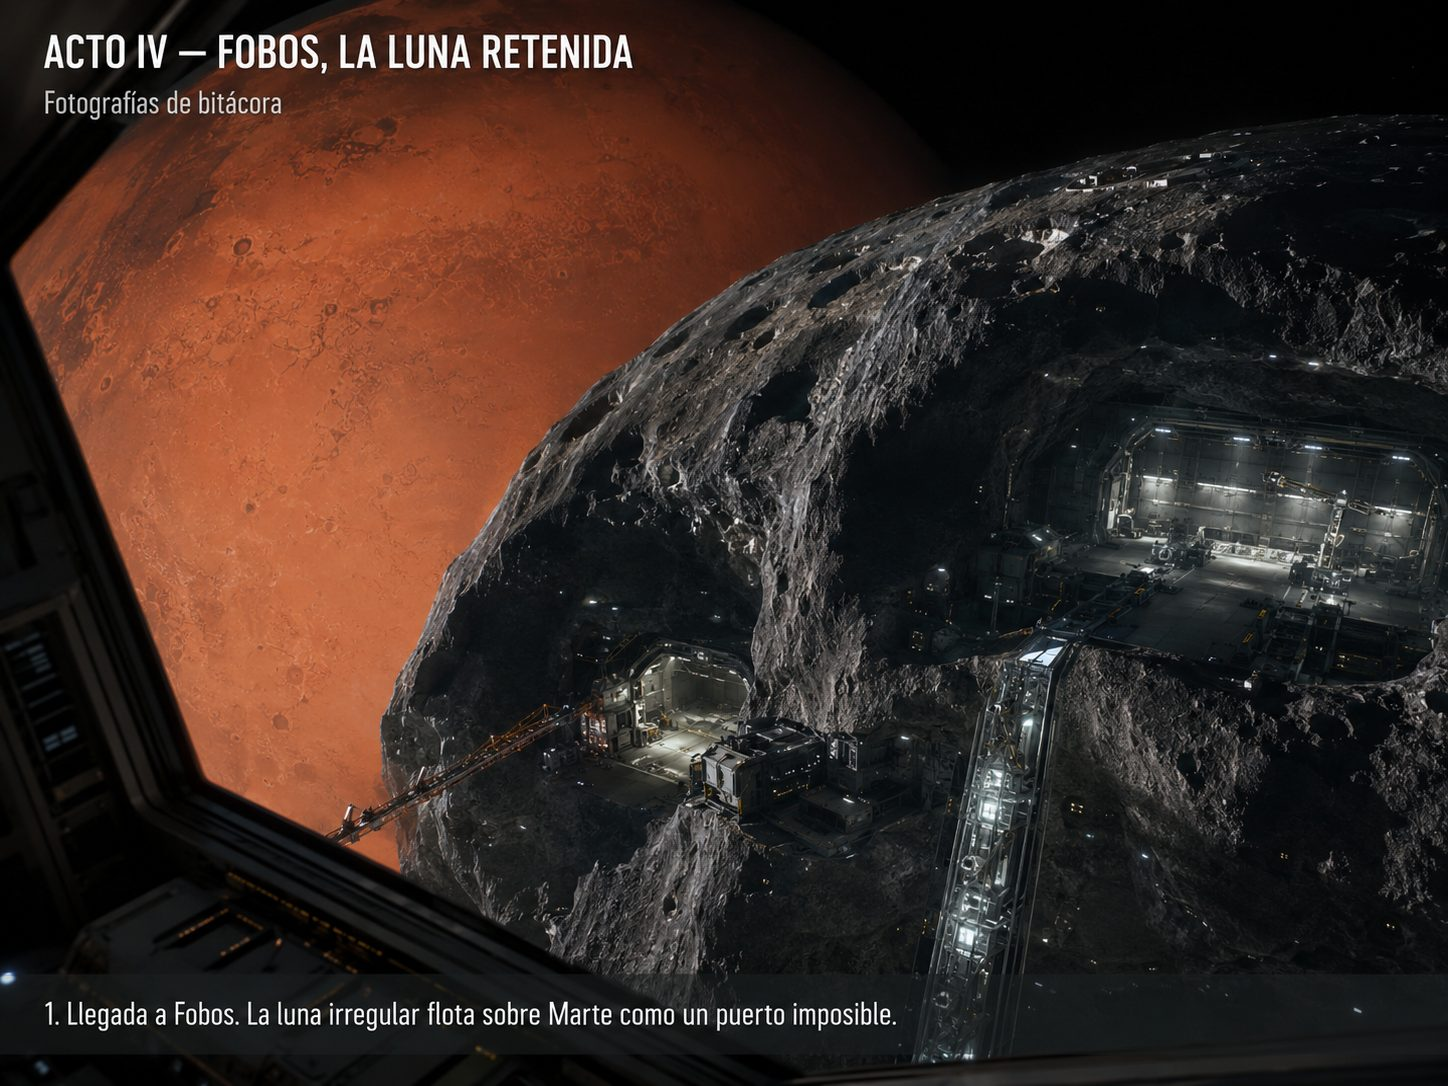
\includegraphics[width=0.9\textwidth]{04_1_llegadaafobosunabaseenmarte.jpg}
\end{figure}

La Estación Fobos estaba excavada en la propia luna. No se posaba sobre ella: la mordía.

Había hangares abiertos en cráteres, depósitos enterrados bajo metros de roca, torres de alineación asomando entre formaciones antiguas, plataformas de descenso a Marte y, sobre todo, los *\textit{correctores orbitales}*.

\begin{figure}[h]
\centering
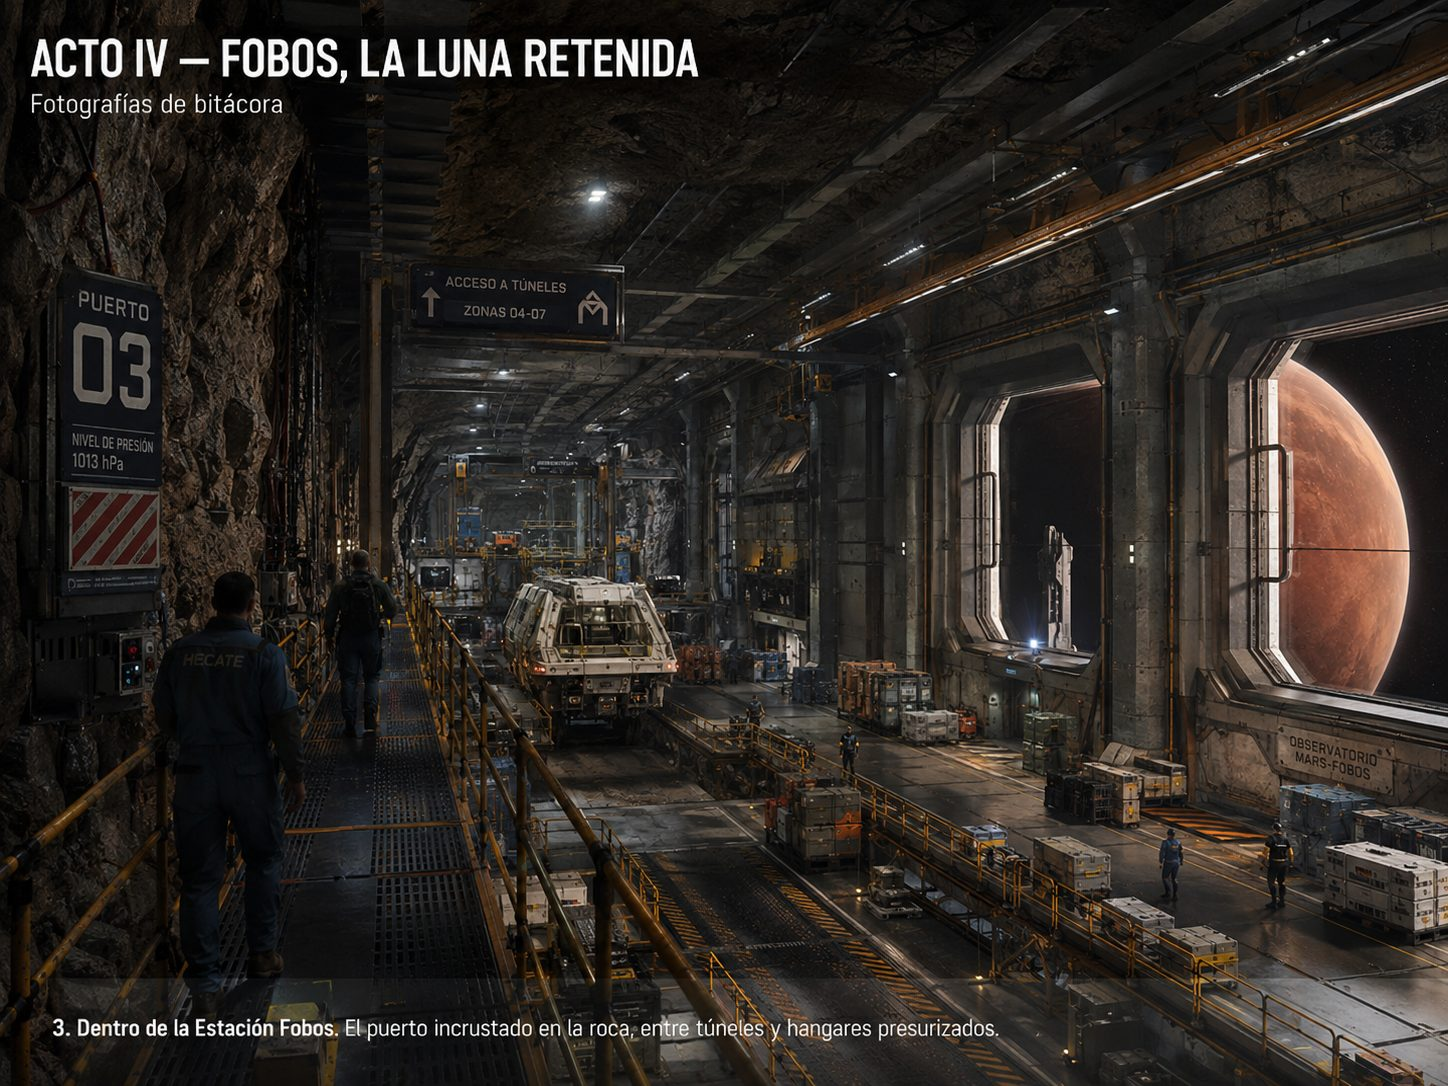
\includegraphics[width=0.9\textwidth]{04_2_estacinsubterrneaenfobos.jpg}
\end{figure}

Los vi durante la maniobra de aproximación: enormes motores anclados a la roca mediante estructuras que parecían raíces metálicas creciendo hacia abajo. Algunos estaban apagados, enfriando. Otros emitían plumas azules y constantes, tan finas que desde la distancia parecían casi decorativas.

\begin{figure}[h]
\centering
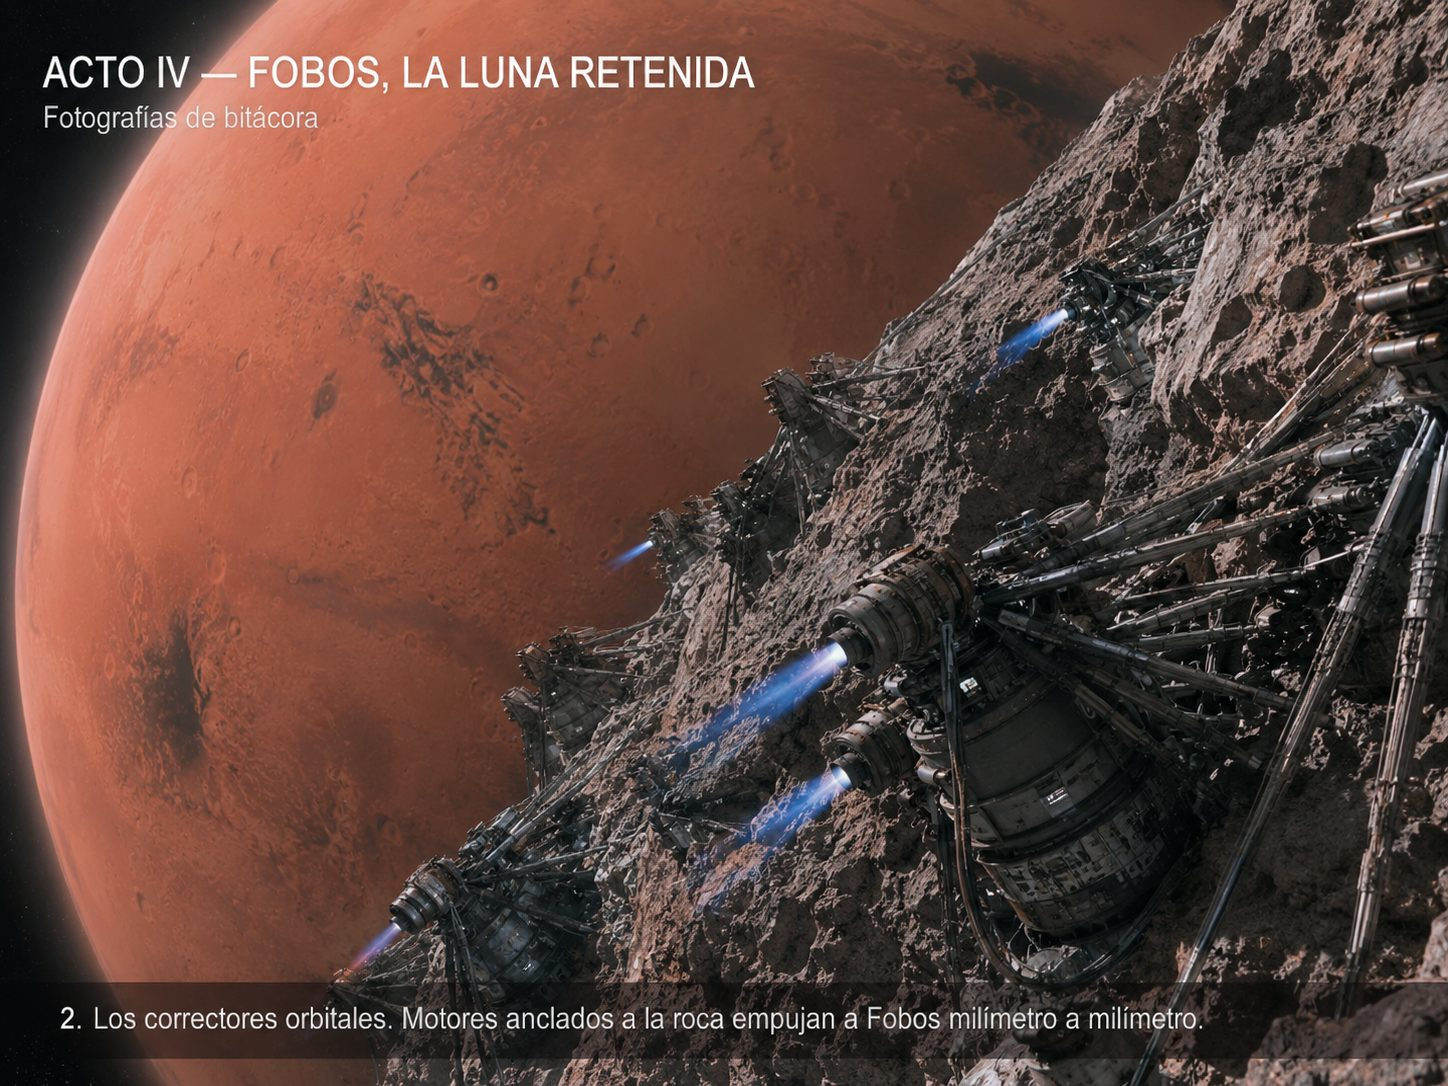
\includegraphics[width=0.9\textwidth]{04_3_fobosmotoresancladosycorrientesenergticas.jpg}
\end{figure}

No lo eran.

El técnico que me acompañó en el tour de instalaciones lo explicó señalando uno de los motores:

—Si no hacemos nada, Fobos cae. No mañana, ni en mil años, pero cae. La órbita se degrada. Cada año que pasa, Fobos está un poco más cerca de Marte. En algún momento lo alcanzará o se romperá en el límite de Roche. Y ahora es puerto, mina, astillero y archivo. Marte no puede permitirse perderlo.

—¿Lo estáis salvando?

—Lo estamos negociando con la gravedad.

Me pareció una frase hermosa. La apunté con cuidado.

Los correctores no empujaban Fobos como un cohete empuja una nave. Lo acariciaban durante años. Milímetros por segundo añadidos a la velocidad orbital. Toneladas de reacción acumuladas durante décadas. Una paciencia que ninguna generación de ingenieros verá completamente cumplida, porque el trabajo de hoy será continuado por los hijos de sus hijos.

Bajé a Marte durante dos días. No estaba en mi itinerario original, pero el técnico me dijo que nadie cruza Fobos sin tocar el planeta, aunque sea por cortesía. Reservé plaza en la lanzadera de superficie.

La bajada fue tranquila. La atmósfera marciana frenó con suavidad.

\begin{figure}[h]
\centering
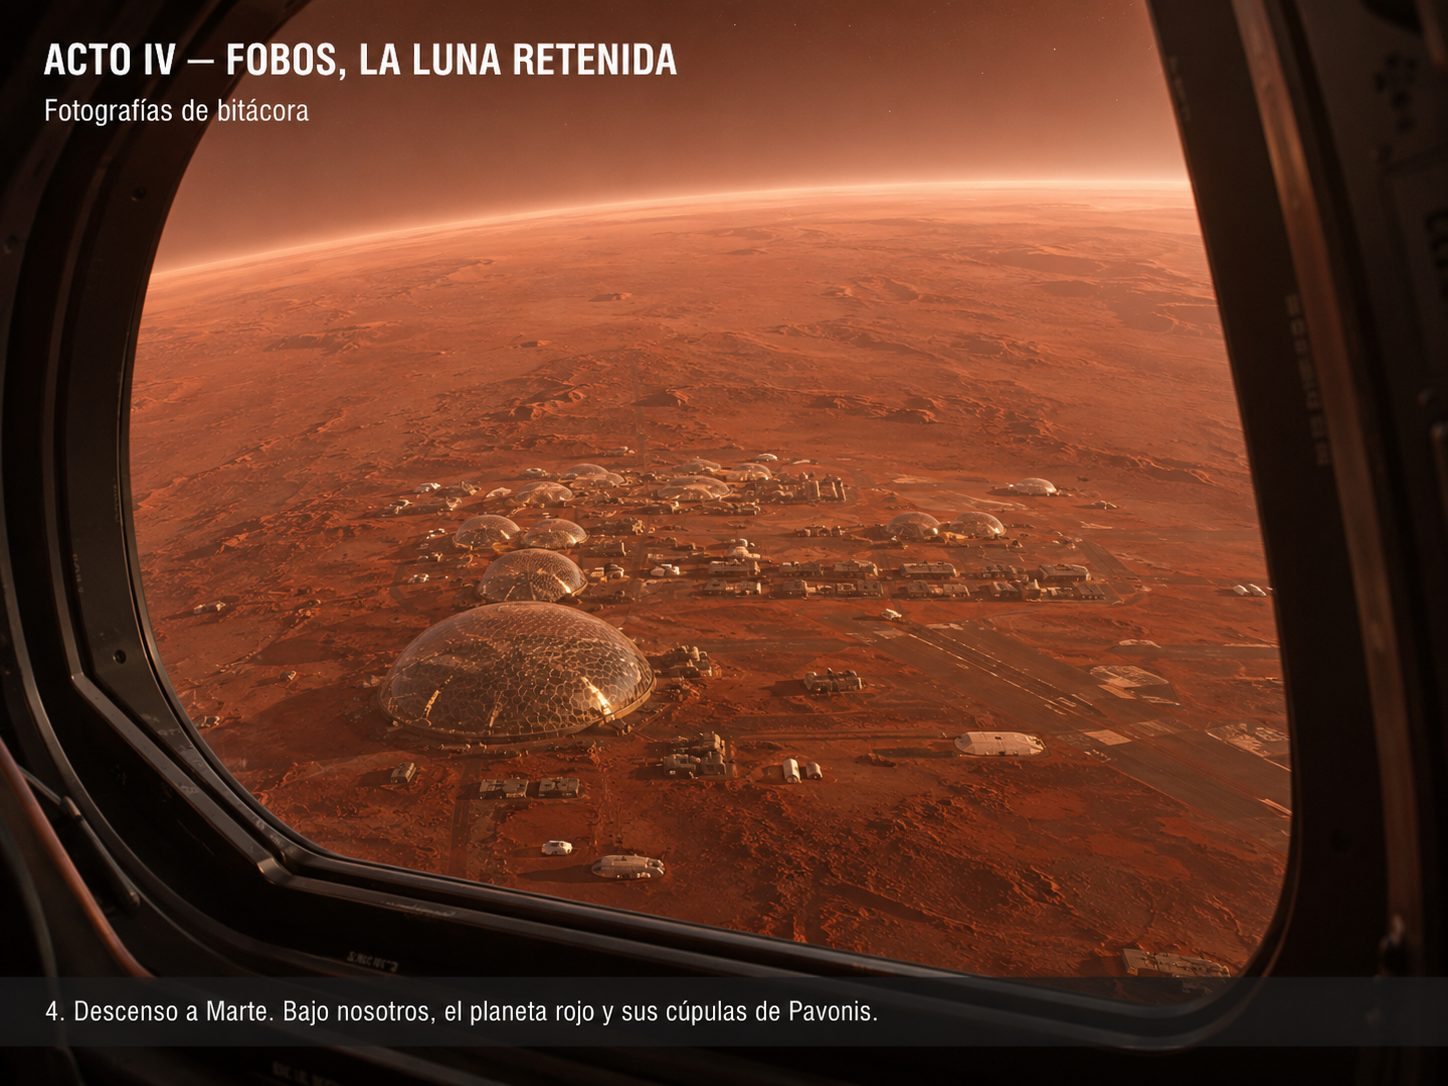
\includegraphics[width=0.9\textwidth]{04_4_descensohacialacoloniamarciana.jpg}
\end{figure}

Las cúpulas de Pavonis aparecieron al fondo, brillando bajo un cielo color salmón, más sutil de lo que esperaba. Salmón no es rojo. Es una variación del naranja que nunca sale bien en las fotografías porque los sensores no saben qué hacer con una luz que no conocen.

\begin{figure}[h]
\centering
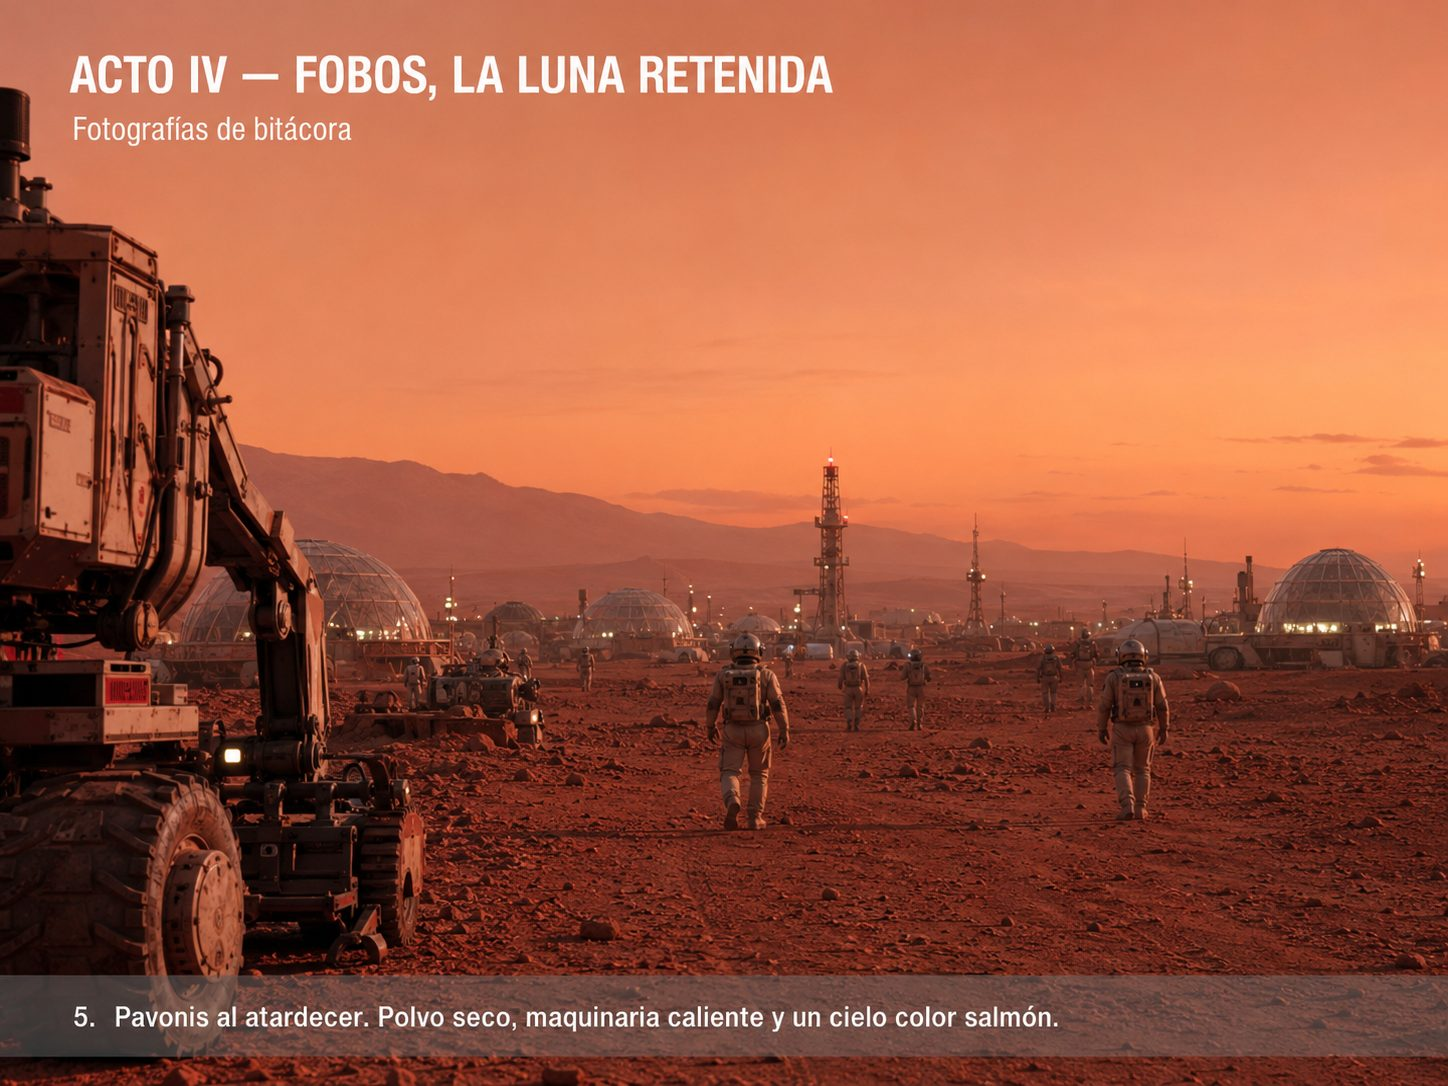
\includegraphics[width=0.9\textwidth]{04_5_pavonisalatardecercoloniamarciana.jpg}
\end{figure}

La superficie marciana olía a polvo seco y maquinaria caliente. La gravedad era ligera, pero no amable: 0,38g te dice que puedes hacer cosas que no puedes. Me cansé más de lo que esperaba.

Por la noche, desde la cúpula exterior de Pavonis, vi Fobos cruzar el cielo.

\begin{figure}[h]
\centering
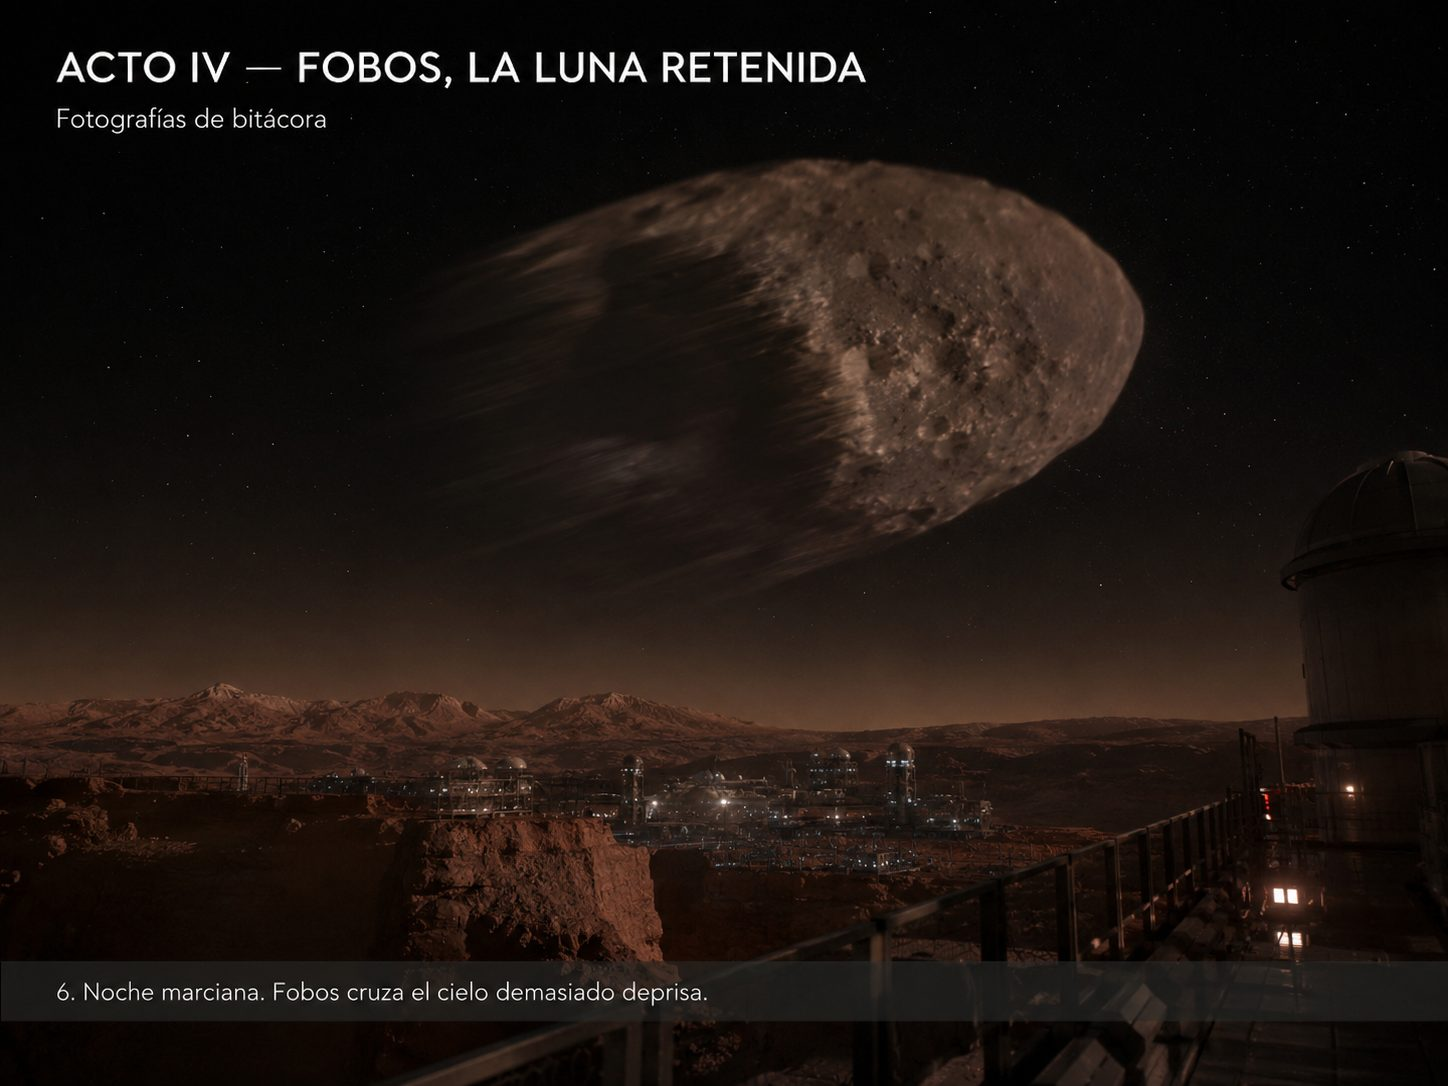
\includegraphics[width=0.9\textwidth]{04_6_coloniamarcianabajofobos.jpg}
\end{figure}

Rápido. Demasiado rápido. Cruzó el cielo en poco más de cuatro horas, de horizonte a horizonte, moviéndose más deprisa que cualquier luna que la física debería permitir a esa distancia.

Y por primera vez entendí por qué una luna puede parecer frágil.

\vspace{1.5em}
\begin{center}$\ast$\quad$\ast$\quad$\ast$\end{center}
\vspace{1.5em}

\chapter*{Acto V — Ceres, el puerto de las cosas pesadas}
\addcontentsline{toc}{chapter}{Acto V — Ceres, el puerto de las cosas pesadas}
\markboth{Acto V — Ceres, el puerto de las cosas pesadas}{Acto V — Ceres, el puerto de las cosas pesadas}

*\textit{Días 13–41. Carguero de fusión eléctrica. Ruta Fobos–Ceres. Llegada: Nodo industrial de Ceres.}*

De Fobos salimos en un cicler clásico.

\begin{figure}[h]
\centering
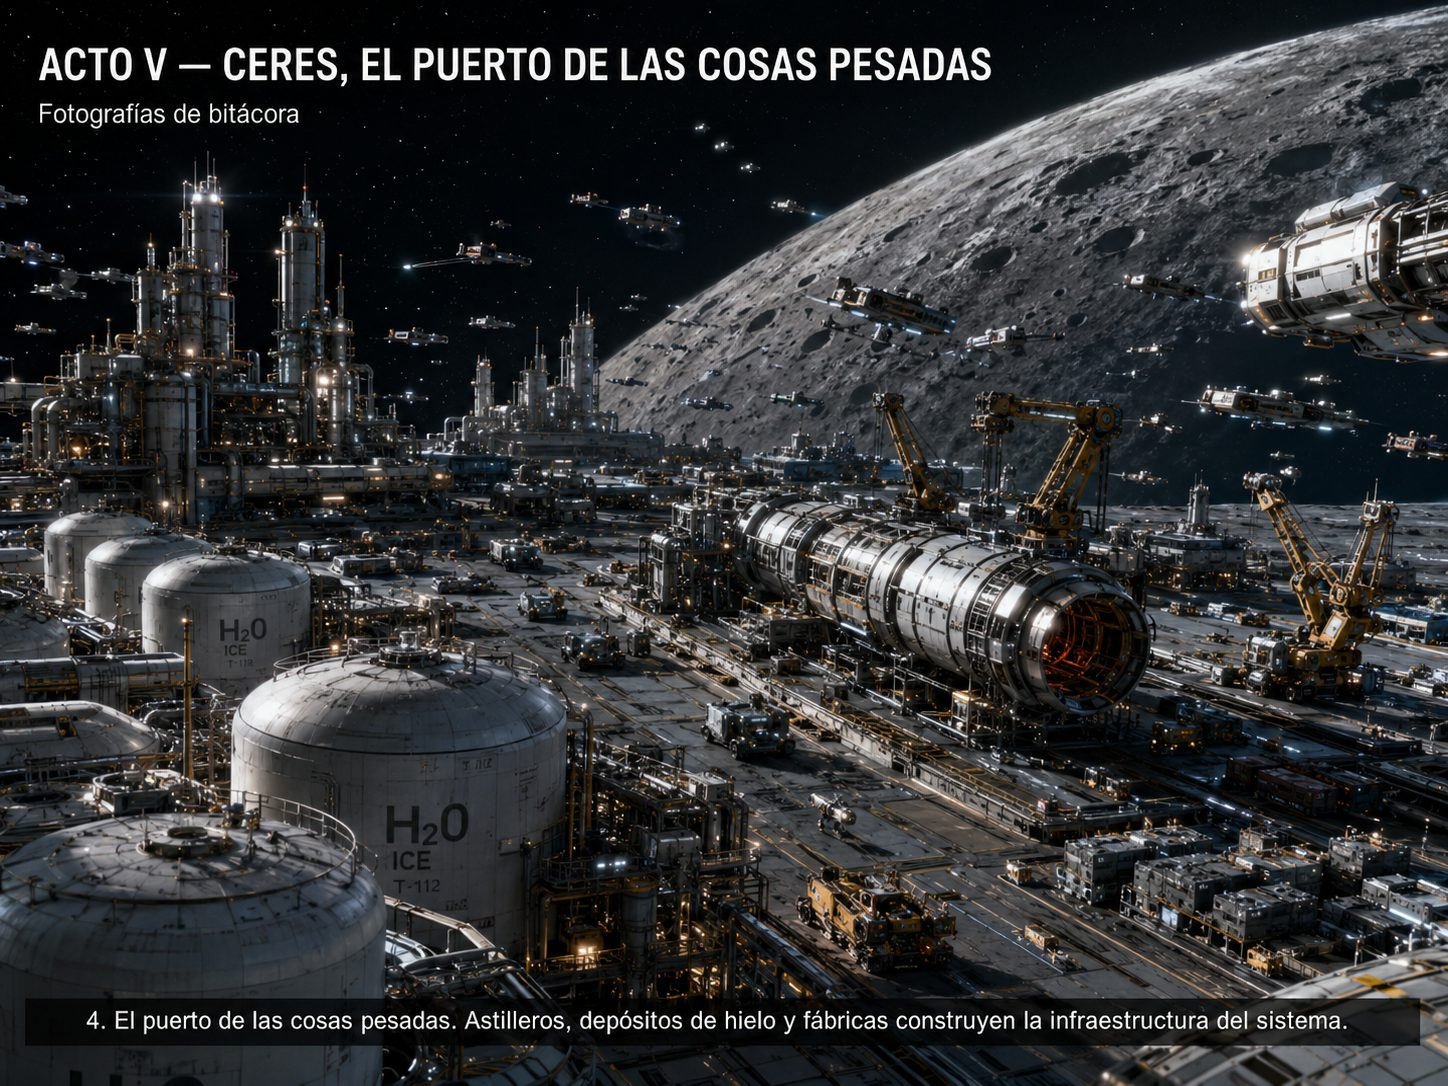
\includegraphics[width=0.9\textwidth]{05_1_puertoindustrialdeceres.jpg}
\end{figure}

No warp. No corredor de campo. Fusión eléctrica lenta, eficiente, aburrida. El tipo de propulsión que lleva cien años funcionando sin que nadie le haga un documental. El capitán lo dijo con un orgullo que me pareció completamente ganado:

—Barato, seguro y casi sin desperdicio.

Tardamos veintinueve días en llegar a Ceres.

Veintinueve días es mucho tiempo cuando tienes poco que hacer. Y a la vez no es nada cuando tienes tiempo para pensar. El interior del carguero olía diferente al Kepler-Sancho: menos pasajeros, más carga. Menos ventanas, más tuberías. El ambiente era el de algo que ha renunciado a parecer cómodo y ha decidido ser útil en su lugar. Gente con mono de trabajo, familias de colonos con los mismos cuatro bultos, mineros de contrato que dormían en cualquier parte con la facilidad de quien ha aprendido que el sueño no espera.

\begin{figure}[h]
\centering
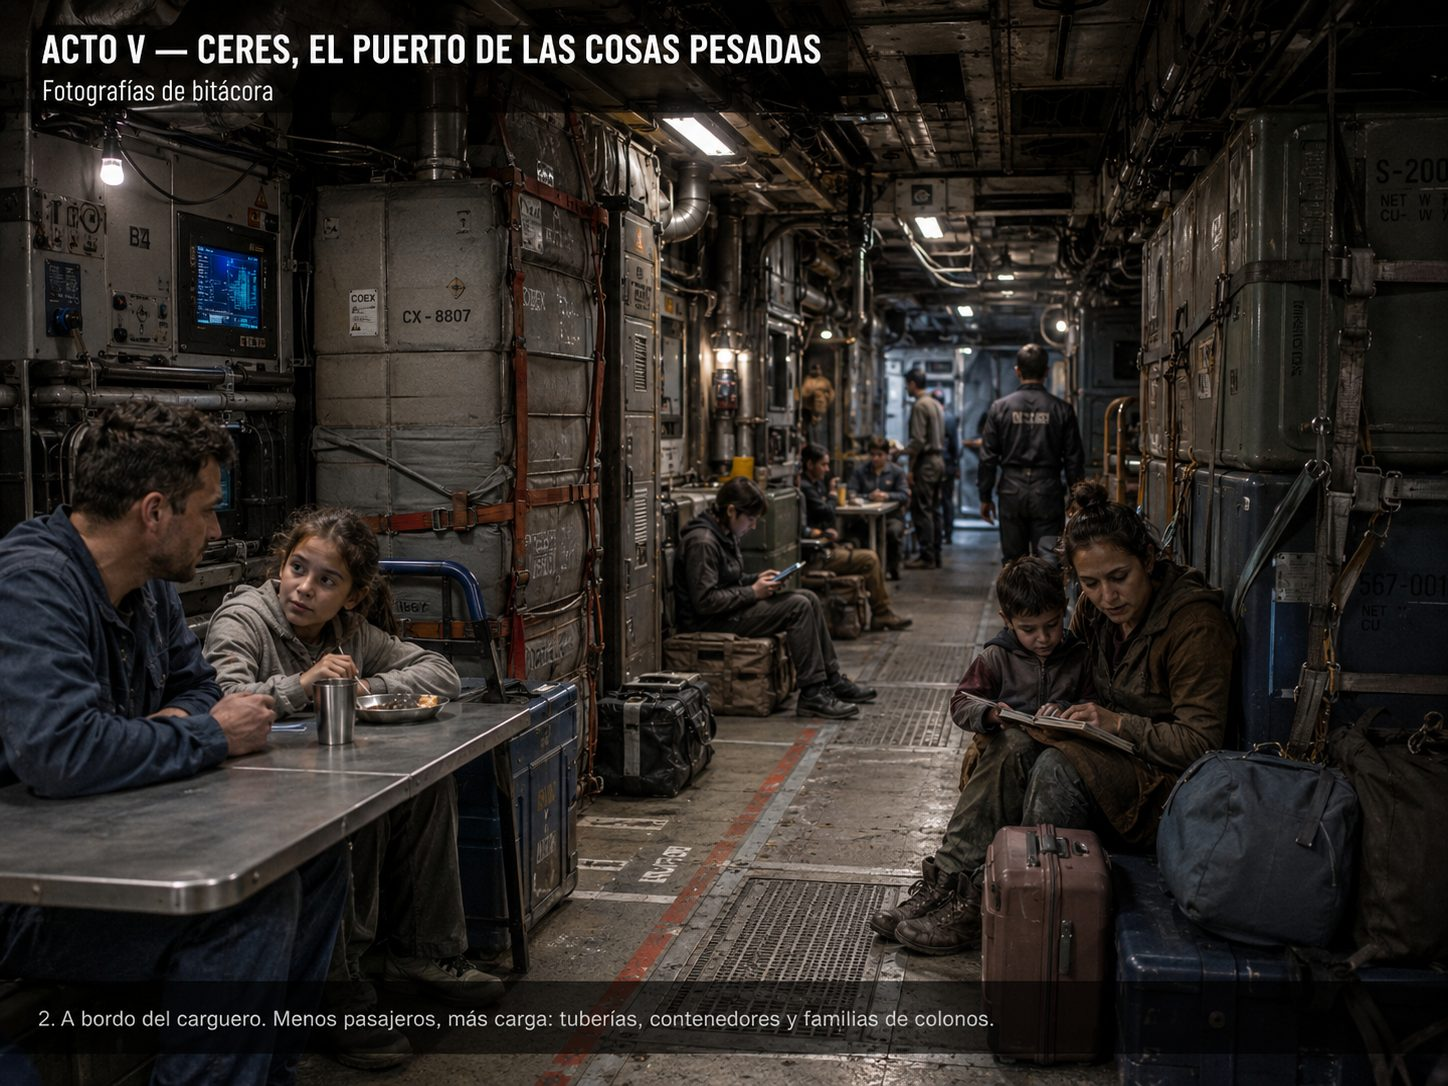
\includegraphics[width=0.9\textwidth]{05_2_abordodelcargueroenceres.jpg}
\end{figure}

Era un barco.

No en el sentido figurado. En el sentido literal del funcionamiento: carga en bodega, pasajeros en cubierta superior, tripulación en sección central, mantenimiento continuo de los sistemas, reuniones diarias para revisar el consumo de propelente. Y como en los barcos de siglos anteriores, había un código de conducta no escrito que todos conocían: no interfieras con la carga, no molestes a la tripulación, cede paso en los pasillos estrechos.

Y entendí la comparación de fondo: aunque existían los aviones, los barcos habían seguido cruzando océanos. Aunque existía el warp, la economía seguía necesitando paciencia. Los cargueros lentos no habían desaparecido porque los rápidos existieran. Habían sobrevivido porque el coste importa más que la velocidad cuando la carga no tiene prisa.

Ceres apareció como una esfera gris, pequeña y vieja. No había nada en ella que dijera «aquí ocurren cosas importantes». Era la apariencia de un planeta que nunca terminó de serlo, con apenas el 0,3\% de la masa de la Tierra, flotando en el cinturón con la discreción de un trabajador que no necesita que lo aplaudan.

\begin{figure}[h]
\centering
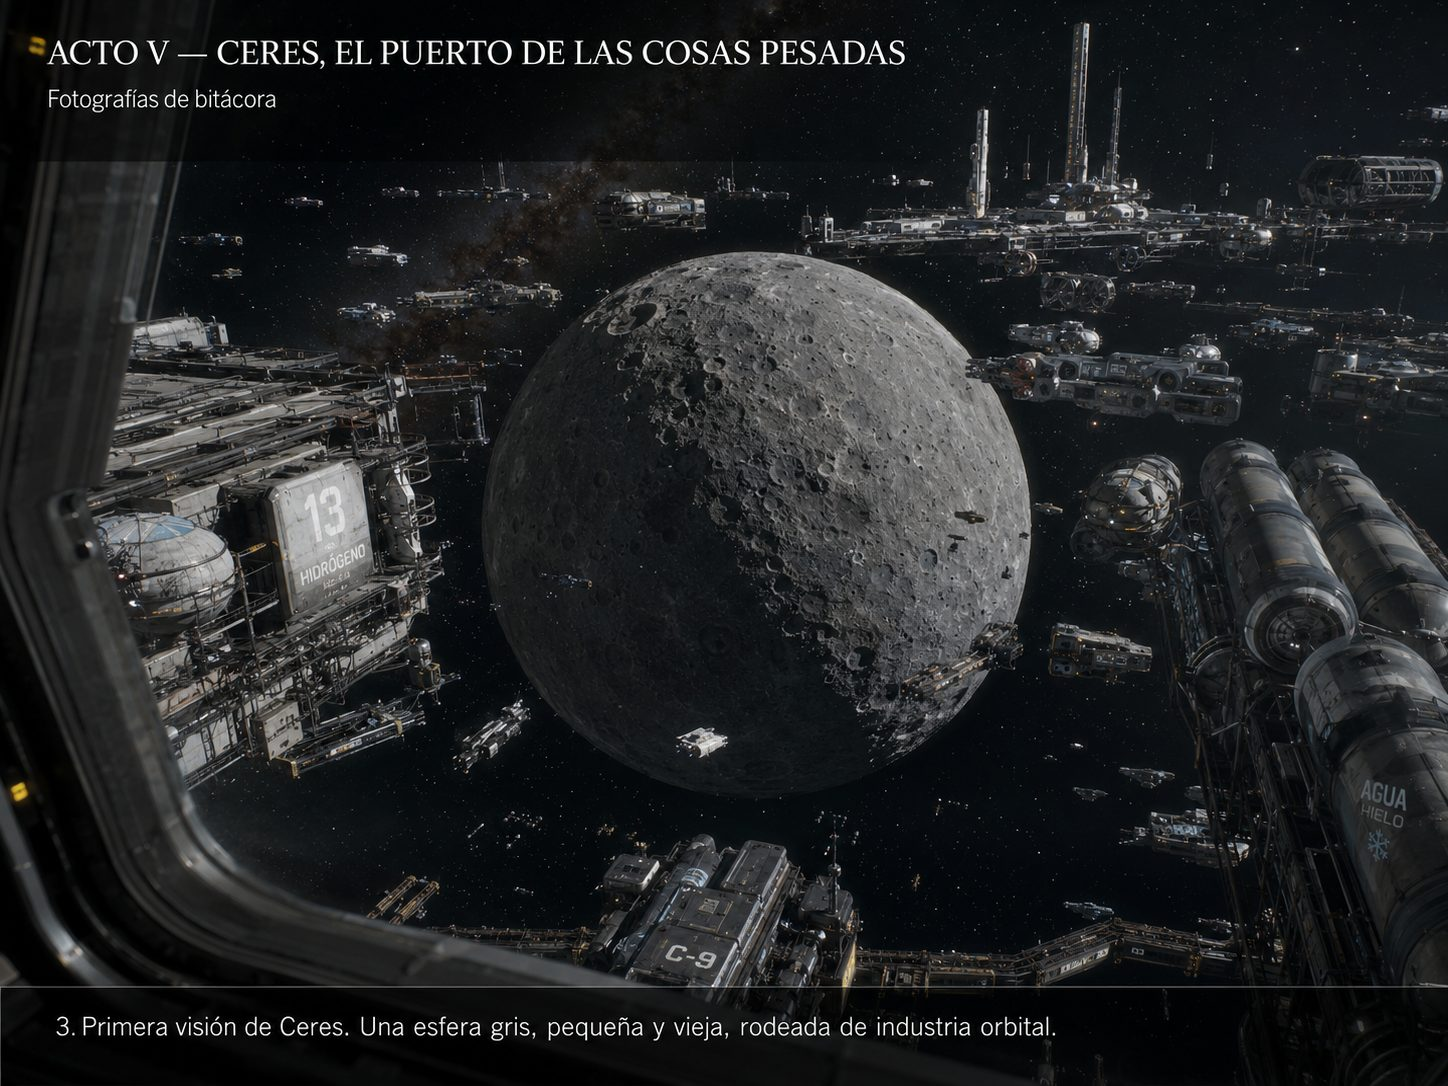
\includegraphics[width=0.9\textwidth]{05_3_actovcereselpuertoindustrial.jpg}
\end{figure}

Pero a su alrededor flotaba el verdadero tesoro.

\begin{figure}[h]
\centering
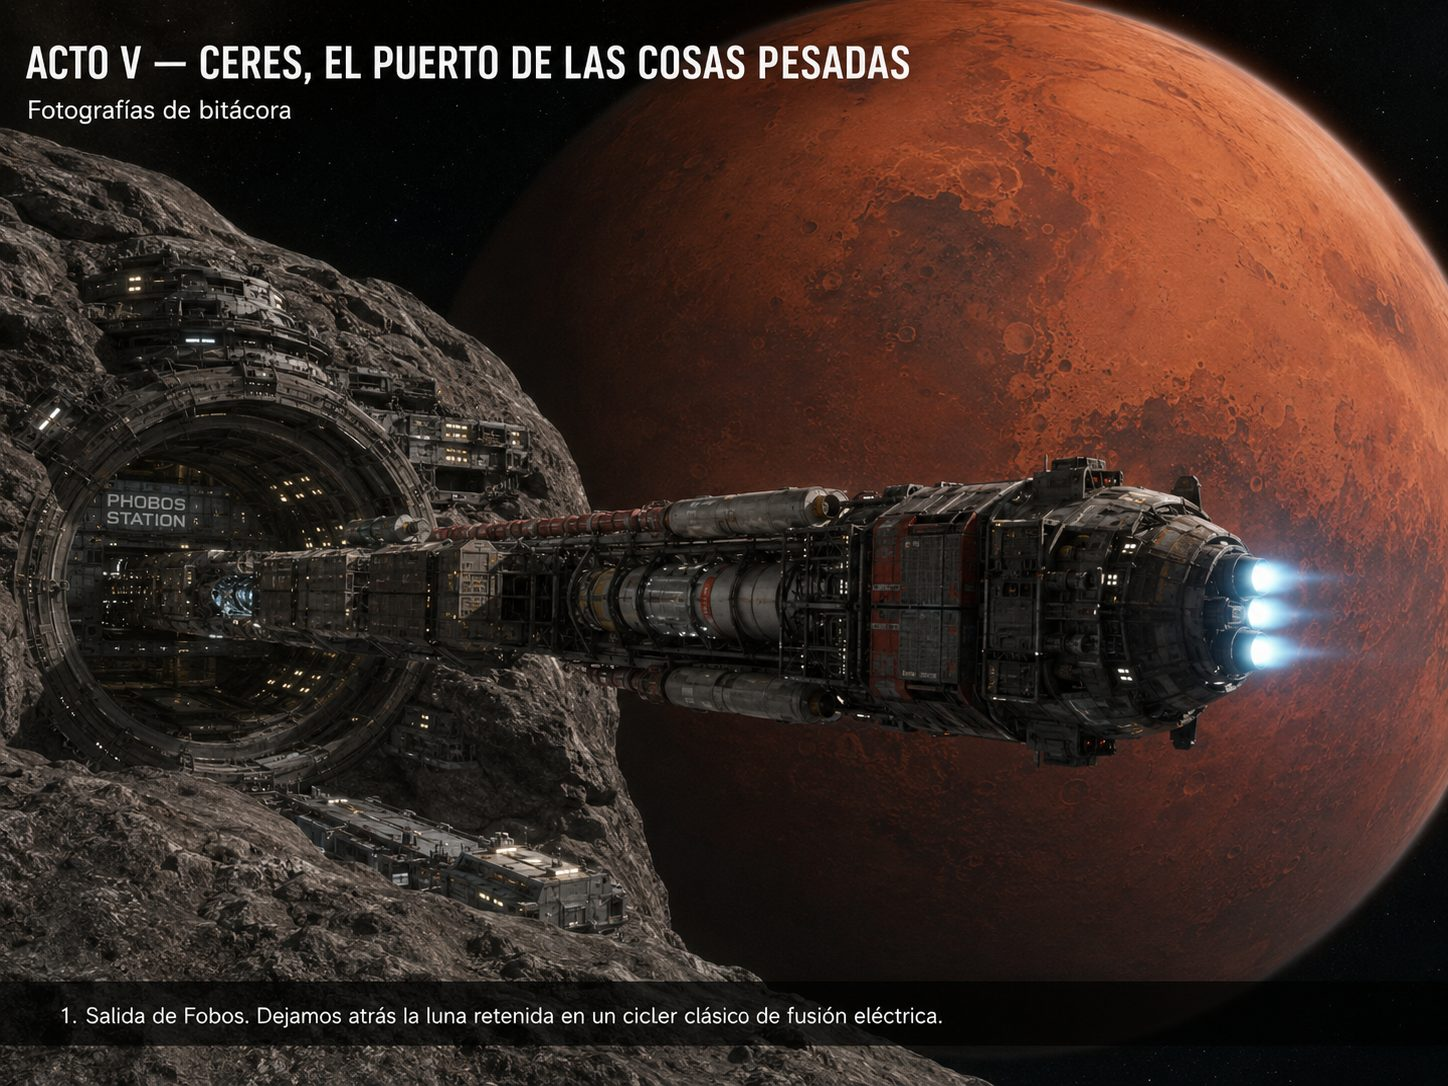
\includegraphics[width=0.9\textwidth]{05_4_puertoindustrialenceres.jpg}
\end{figure}

Astilleros. Fábricas. Depósitos de hielo que brillaban en el espacio con la superficie plana de algo que ha sido cortado con precisión. Cilindros en construcción, algunos del tamaño de bloques de ciudad. Enjambres de drones mineros circulando en patrones geométricos que desde lejos parecían migración animal. Allí no se construían sueños. Se construían vigas, tanques, radiadores, blindajes, anillos. Las piezas de todo lo demás.

Un ingeniero me enseñó una sección incompleta de curvatura en el astillero exterior. Era una pieza curva de casi cuatrocientos metros, con la pátina mate del metal espacial trabajado: gris oscuro con reflejos verdes donde el vacío había oxidado la superficie a su manera.

\begin{figure}[h]
\centering
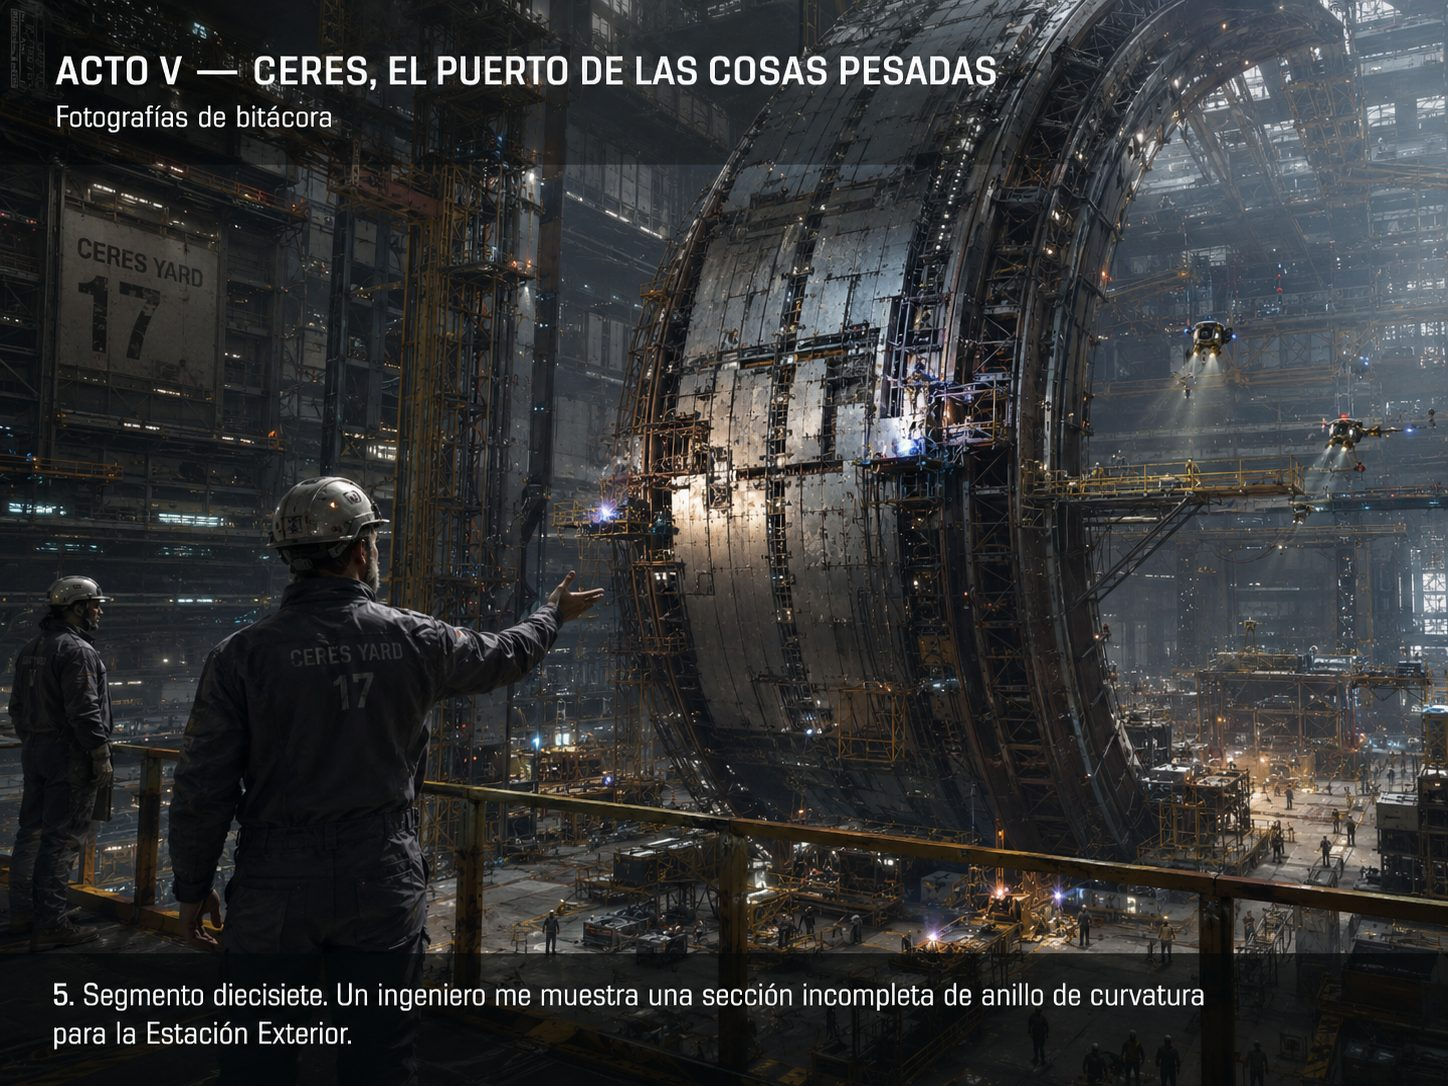
\includegraphics[width=0.9\textwidth]{05_5_laconstruccindelanilloenceres.jpg}
\end{figure}

—Esto irá a la Estación Exterior —dijo—. Segmento diecisiete de la tercera matriz.

—¿Y cuántas piezas tiene la matriz?

—Novecientas sesenta.

No respondí nada. Miré el segmento. Cuatrocientos metros de metal preciso, fabricado aquí, en este punto gris del cinturón de asteroides, que iba a viajar meses hasta La Exterior para encajar como una pieza en algo que lanzaría naves hacia otras estrellas.

Él sonrió ante mi silencio.

—Por eso las estrellas son caras.

\begin{figure}[h]
\centering
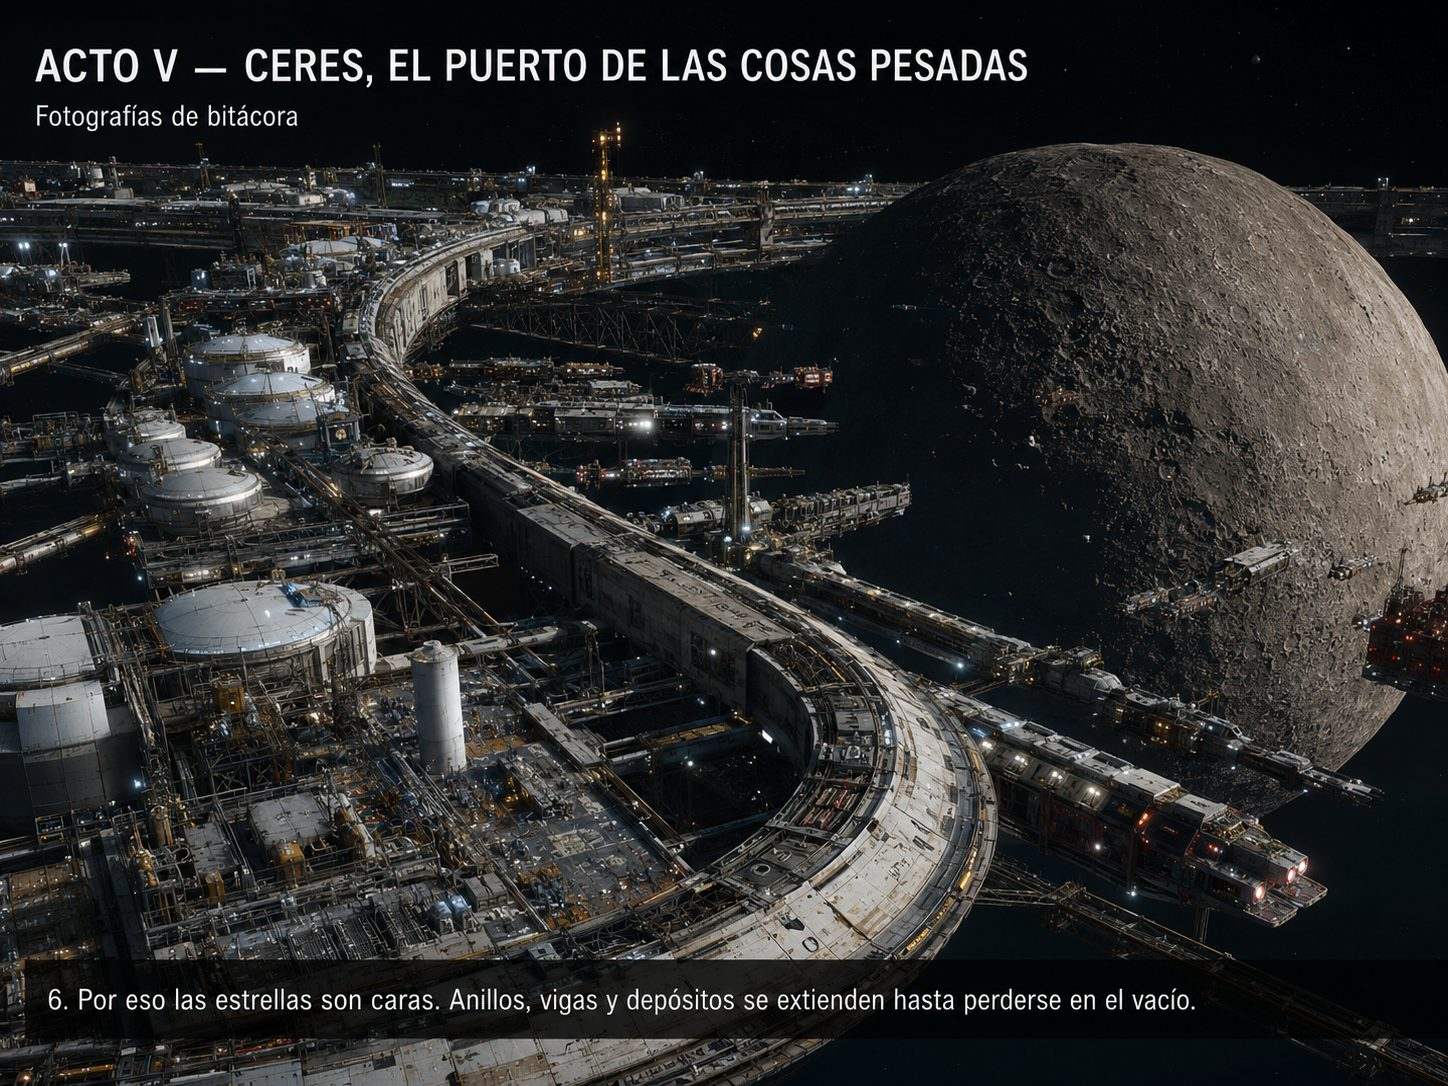
\includegraphics[width=0.9\textwidth]{05_6_puertoorbitalenceres.jpg}
\end{figure}

\vspace{1.5em}
\begin{center}$\ast$\quad$\ast$\quad$\ast$\end{center}
\vspace{1.5em}

\chapter*{Acto VI — Calisto y el silencio de Júpiter}
\addcontentsline{toc}{chapter}{Acto VI — Calisto y el silencio de Júpiter}
\markboth{Acto VI — Calisto y el silencio de Júpiter}{Acto VI — Calisto y el silencio de Júpiter}

*\textit{Días 42–62. Cicler de campo. Ruta Ceres–Calisto. Puerto seguro del sistema joviano.}*

Desde Ceres tomamos un cicler de campo hacia Calisto.

El trayecto duró veinte días. Veinte días durante los cuales el Sol fue reduciéndose gradualmente: primero demasiado brillante para mirarlo, luego un disco visible, luego un punto de luz que daba calor suficiente para los sistemas pero que ya no calentaba las superficies que tocaba. Estábamos cruzando la frontera entre el sistema solar interior y el exterior. No hay una línea marcada. Solo hay una sensación progresiva de que la distancia ha cambiado de naturaleza.

Júpiter no se visita. Júpiter se sobrevive desde lejos.

\begin{figure}[h]
\centering
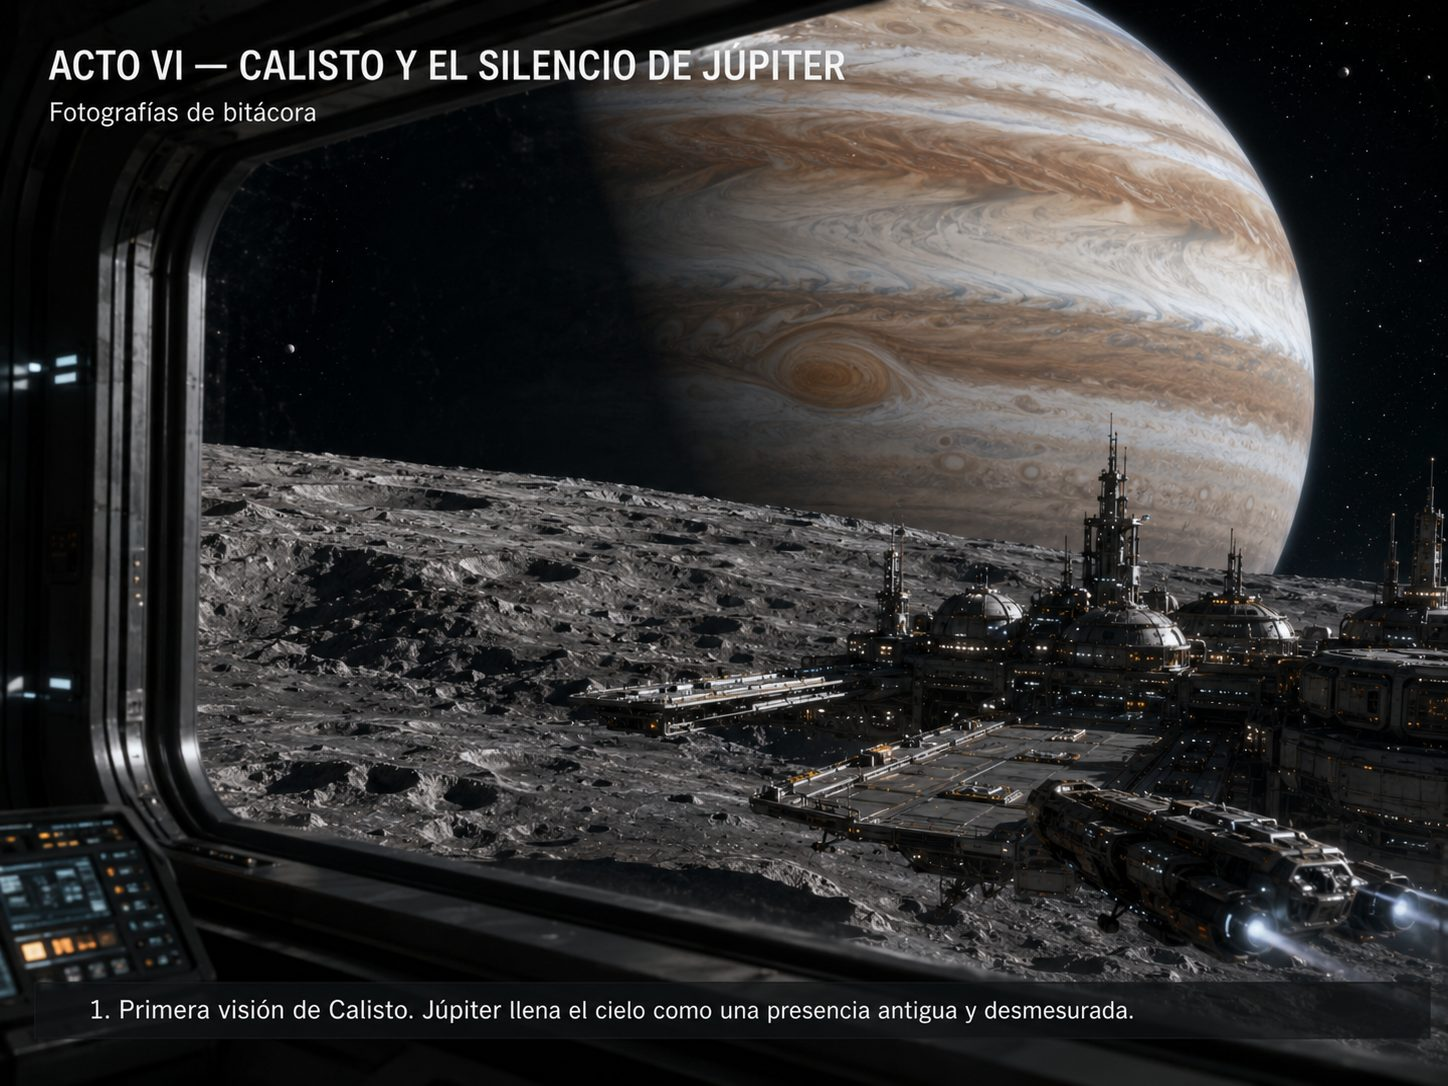
\includegraphics[width=0.9\textwidth]{06_1_calistoyelsilenciodejpiter.jpg}
\end{figure}

Calisto era el puerto seguro del sistema joviano: lo bastante lejos de la radiación brutal de las lunas internas, lo bastante cerca para explotar recursos, estudiar lunas y servir de escala exterior. Lo bastante discreto para que nadie lo mirara con envidia. Toda la grandiosidad de estar en el sistema de Júpiter sin ninguno de los riesgos de acercarse demasiado.

Cuando Júpiter apareció por la ventana, nadie habló.

\begin{figure}[h]
\centering
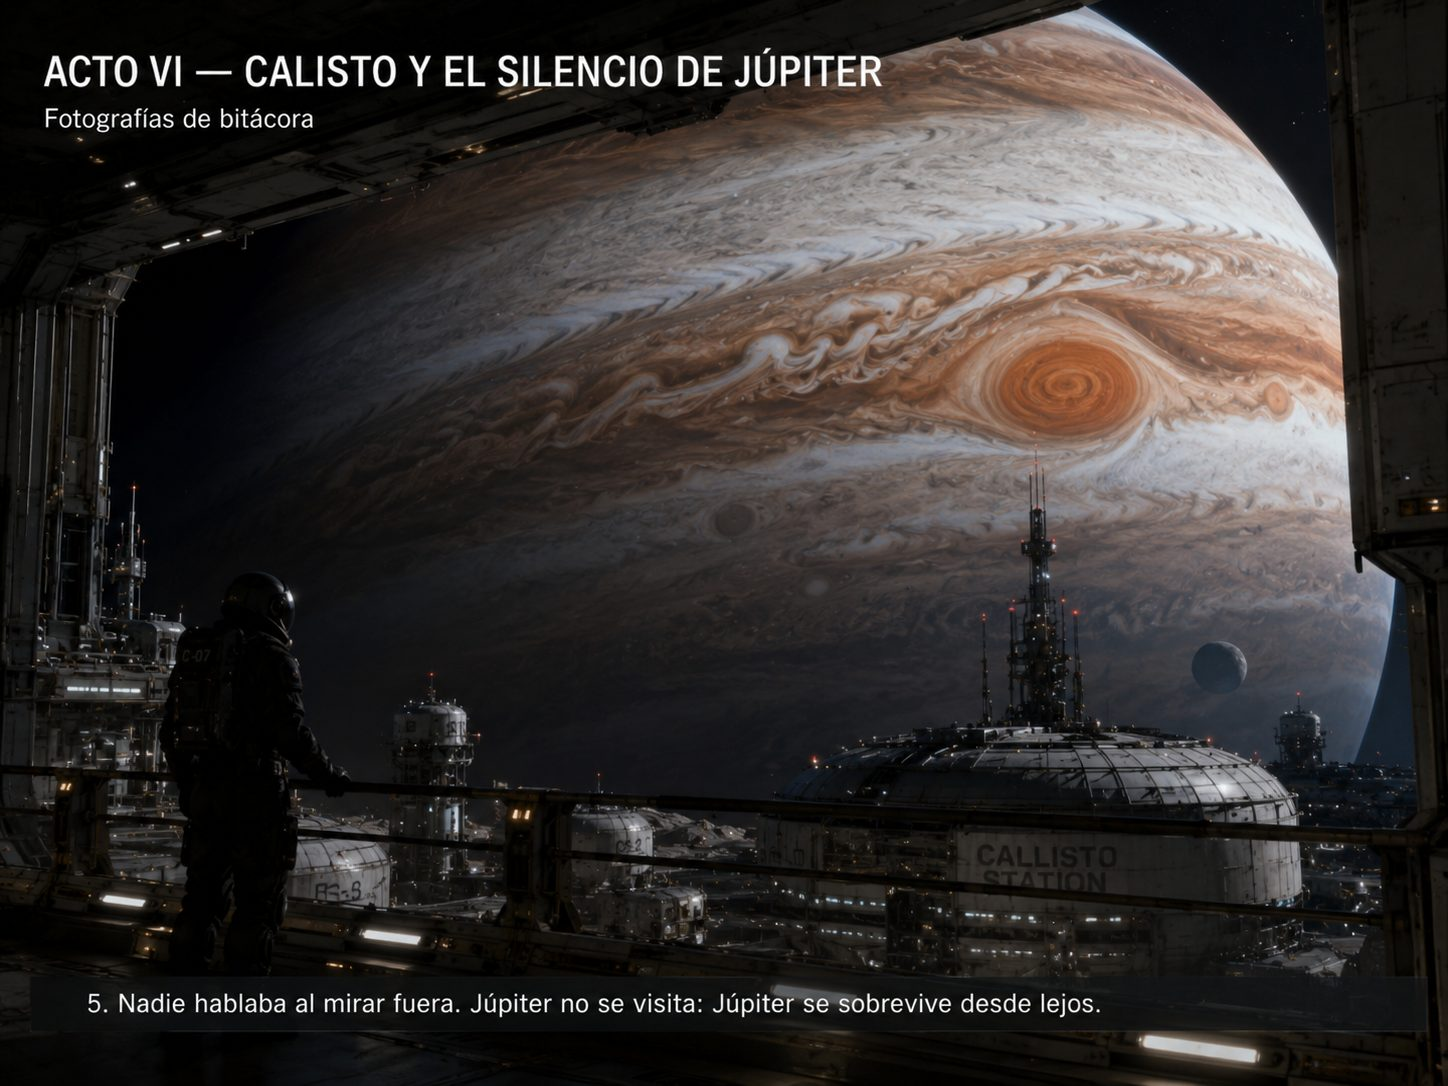
\includegraphics[width=0.9\textwidth]{06_2_vistaespacialdesdelaestacincallisto.jpg}
\end{figure}

Hay cosas que no admiten comentario porque cualquier palabra las empequeñece. Júpiter era una de ellas. La Gran Mancha Roja era visible incluso a simple vista desde esta distancia: un ojo antiguo, girando desde antes de que nuestra especie supiera escribir, antes de que supiéramos hablar, probablemente desde antes de que existiéramos. A su alrededor, las bandas atmosféricas se plegaban como tejidos vivos, en movimiento lento que solo percibes si miras durante un rato y luego apartas los ojos: cuando vuelves, algo ha cambiado.

Calisto, en cambio, era oscuro, lleno de impactos, cubierto de instalaciones bajas y discretas. No había arrogancia arquitectónica allí. Todo estaba enterrado, blindado o duplicado. La regla de diseño parecía ser: si algo puede fallar, ponlo bajo tierra. Si no puede ponerse bajo tierra, ponlo lejos de lo demás. Si no puede estar lejos, construye dos.

\begin{figure}[h]
\centering
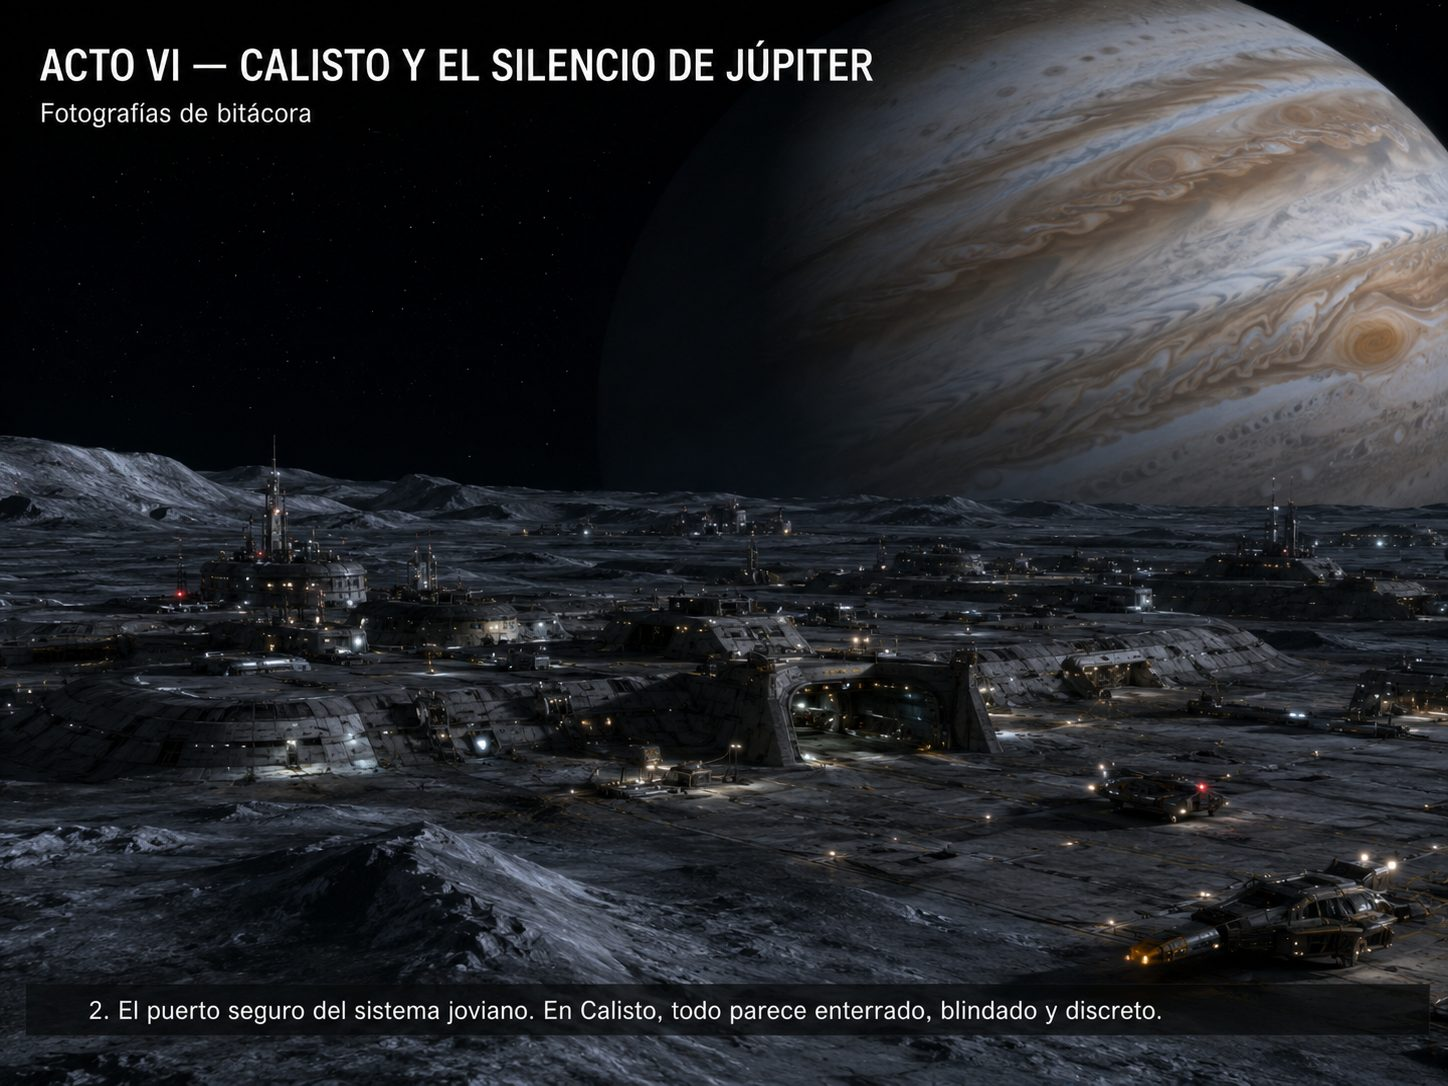
\includegraphics[width=0.9\textwidth]{06_3_puertoseguroencalisto.jpg}
\end{figure}

Era la arquitectura del miedo inteligente.

\begin{figure}[h]
\centering
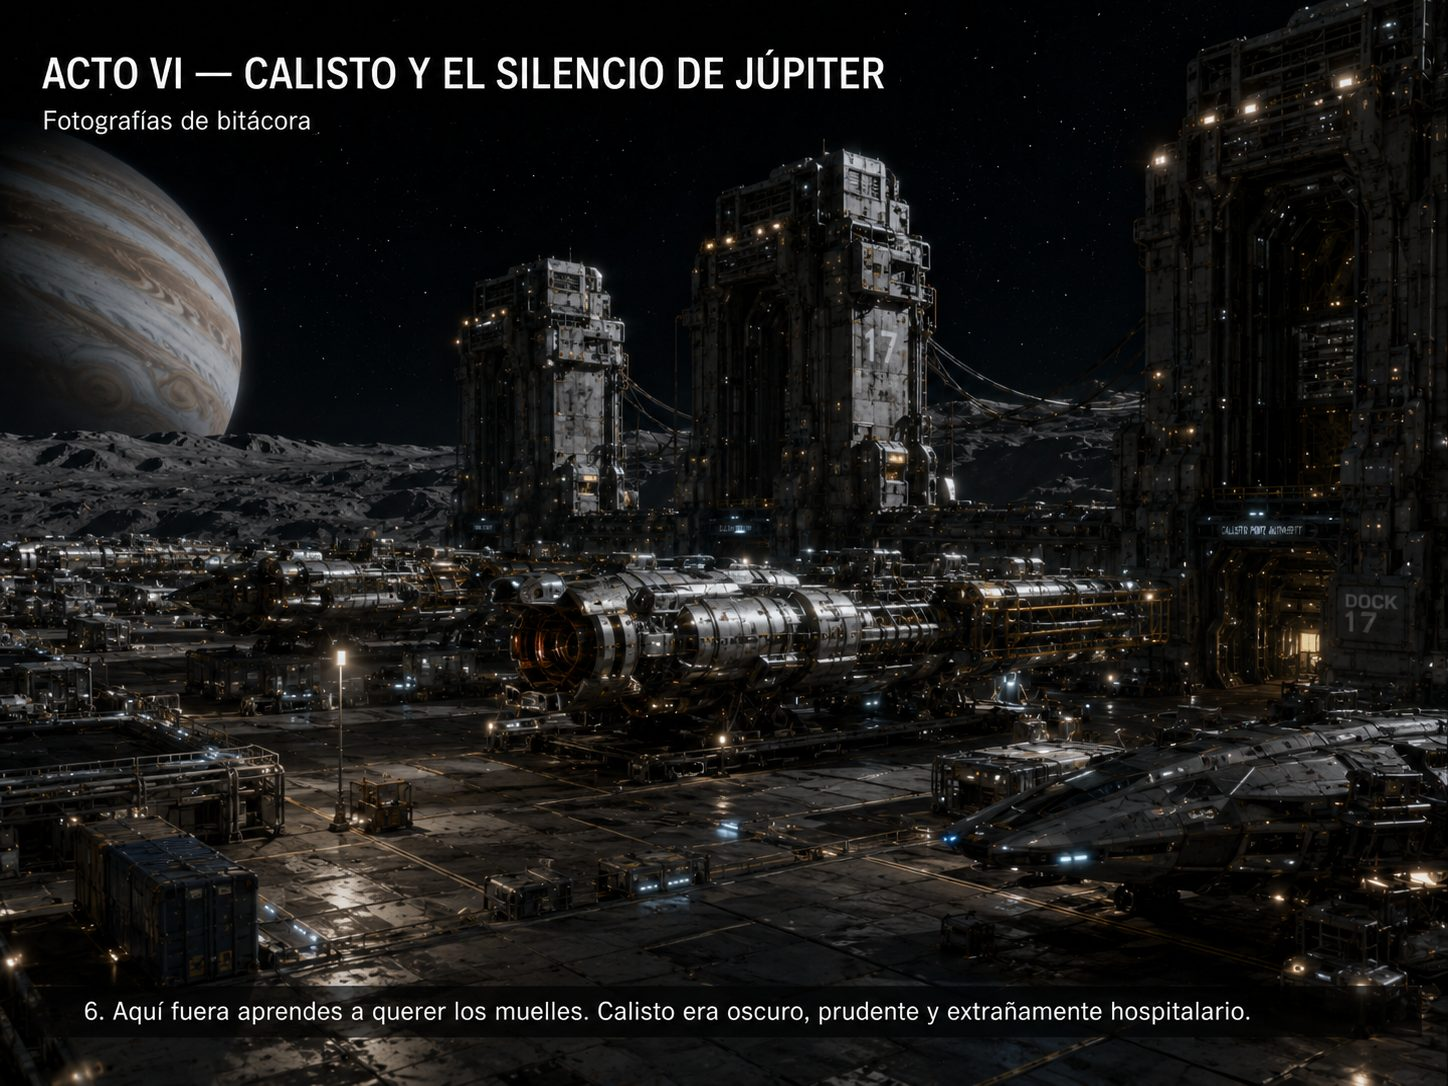
\includegraphics[width=0.9\textwidth]{06_4_puertoespacialencalisto.jpg}
\end{figure}

En el bar del puerto conocí a una piloto de rutas exteriores. Se llamaba Mara y llevaba doce años sin bajar a un planeta.

\begin{figure}[h]
\centering
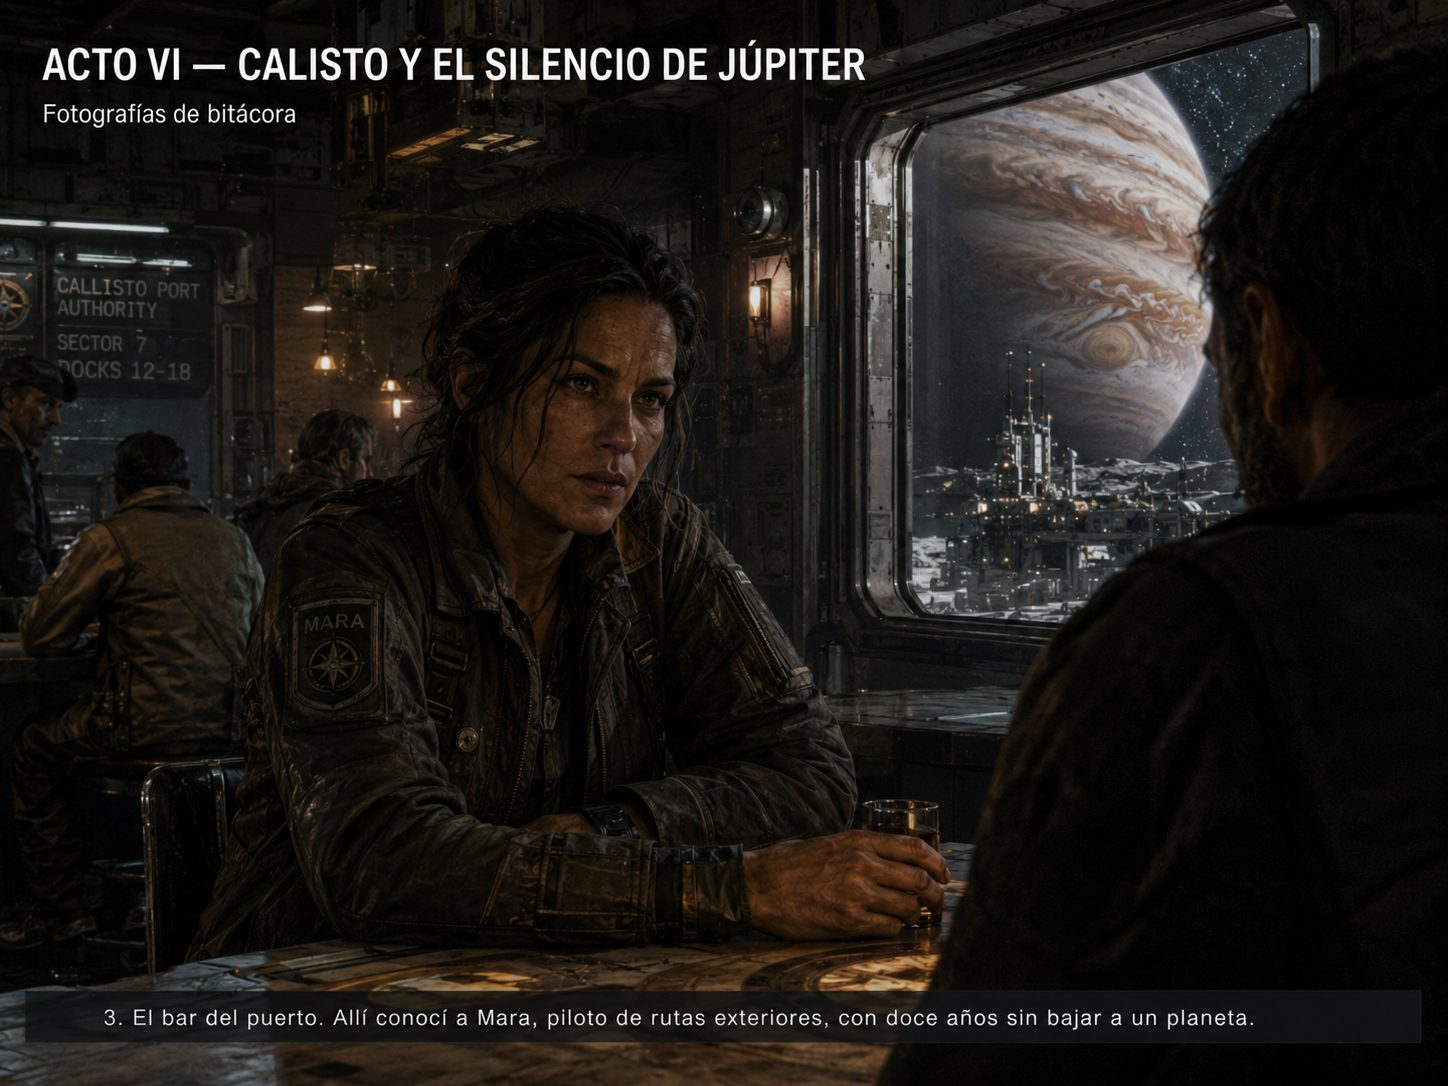
\includegraphics[width=0.9\textwidth]{06_5_elbardelpuertoencalisto.jpg}
\end{figure}

Doce años. Lo calculé mientras me lo decía: casi un tercio de su vida adulta sin gravedad real, sin suelo que no fuera suelo de cubierta, sin cielo abierto. Pero lo decía sin drama, con la tranquilidad de quien ha llegado a una conclusión que le funciona bien.

—Los planetas son pozos —me dijo, con la copa en la mano y mirando hacia la ventana que daba a Júpiter—. Bonitos, sí. Pero pozos. Aquí fuera aprendes a querer los muelles.

\begin{figure}[h]
\centering
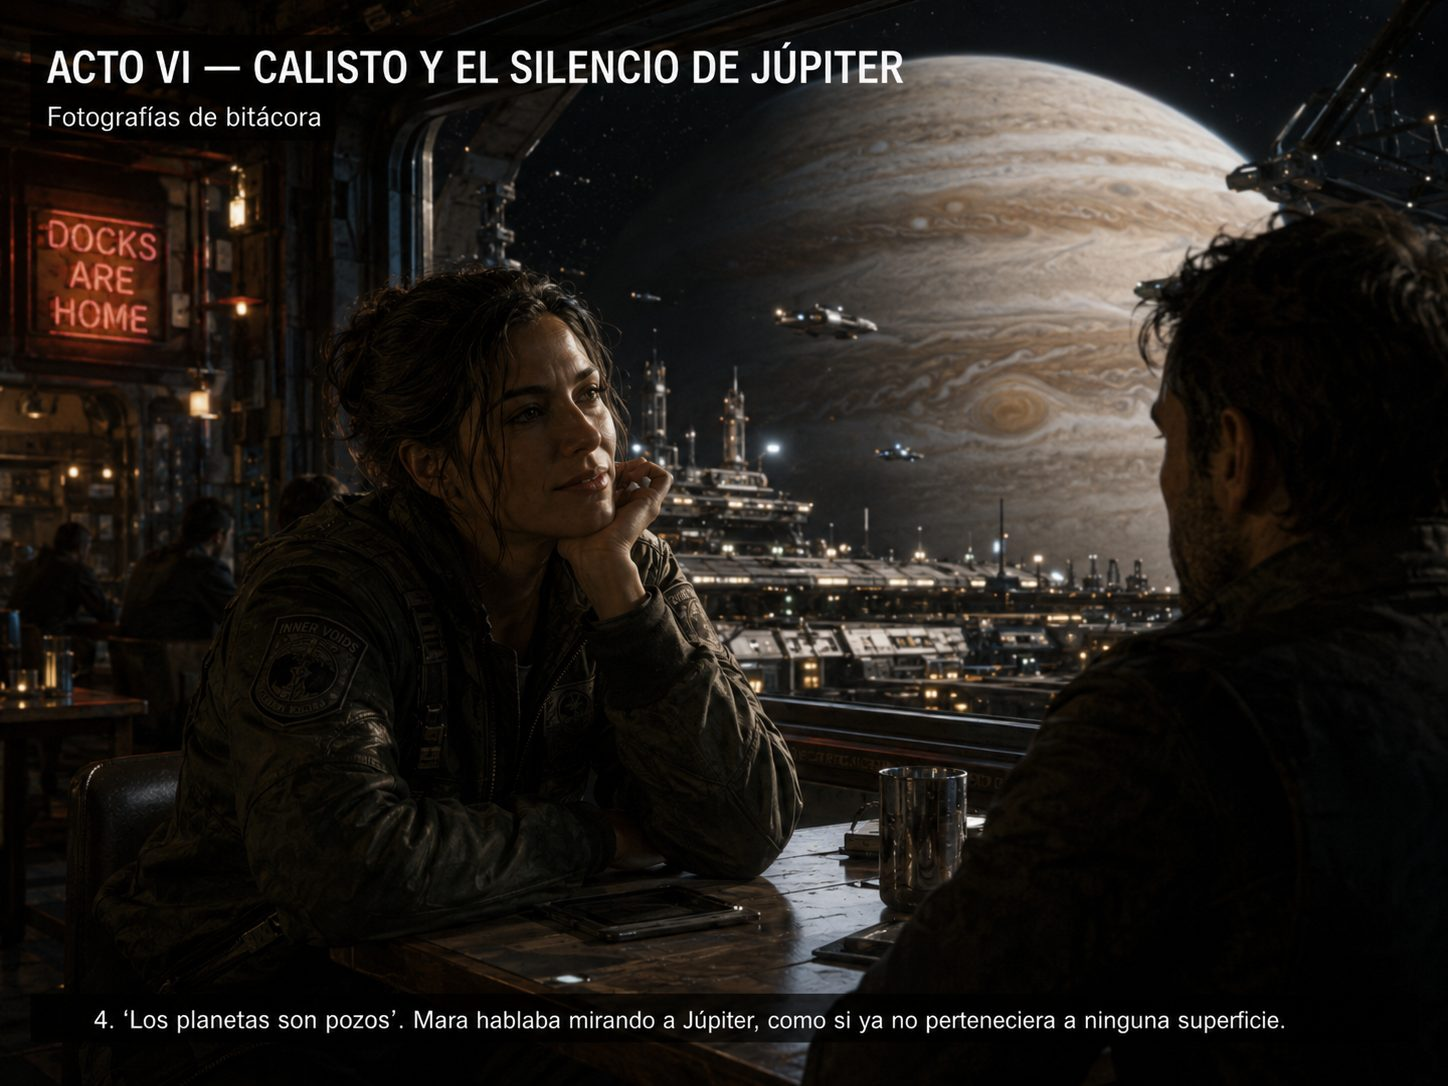
\includegraphics[width=0.9\textwidth]{06_6_calistoyelsilenciodejpiterbar2.jpg}
\end{figure}

Le pregunté si había ido alguna vez a la Estación Warp Exterior.

—Dos veces. Una llevando carga. Otra llevando cadáveres.

Esperé un momento por si continuaba. No continuó.

—¿Qué pasó?

—Accidente de curvatura en un prototipo. No fue nada que no estuviera en el manual de riesgos. Pero fue un accidente de curvatura, y ya sabes cómo son esas cosas: no queda mucho para enterrar.

No pregunté más. Ella tampoco ofreció más.

En algún momento, mientras Júpiter seguía girando al otro lado del cristal, pensé que Mara llevaba doce años mirando eso desde muelles como este. Que para ella, los planetas eran el lujo innecesario y el espacio era el trabajo real.

No sé cuál de los dos tenía razón. Probablemente los dos.

\vspace{1.5em}
\begin{center}$\ast$\quad$\ast$\quad$\ast$\end{center}
\vspace{1.5em}

\chapter*{Acto VII — Titán, la frontera con atmósfera}
\addcontentsline{toc}{chapter}{Acto VII — Titán, la frontera con atmósfera}
\markboth{Acto VII — Titán, la frontera con atmósfera}{Acto VII — Titán, la frontera con atmósfera}

*\textit{Días 63–83. Ruta Calisto–Titán, tres semanas. Sistema de Saturno.}*

Titán fue la última escala con cielo.

No cielo azul. No cielo abierto. Pero cielo.

Llegamos a través de una ruta Calisto-Titán de tres semanas. Saturno apareció primero, antes que Titán, antes que cualquier otra cosa del sistema: una línea horizontal de imposible belleza, una joya con anillos donde no debía caber tanta geometría. Desde la distancia de llegada no se distinguían los anillos como estructuras individuales sino como un único plano de material que el sol iluminaba desde abajo, creando una gradación de luz que iba del blanco al ocre al casi negro en el borde exterior.

\begin{figure}[h]
\centering
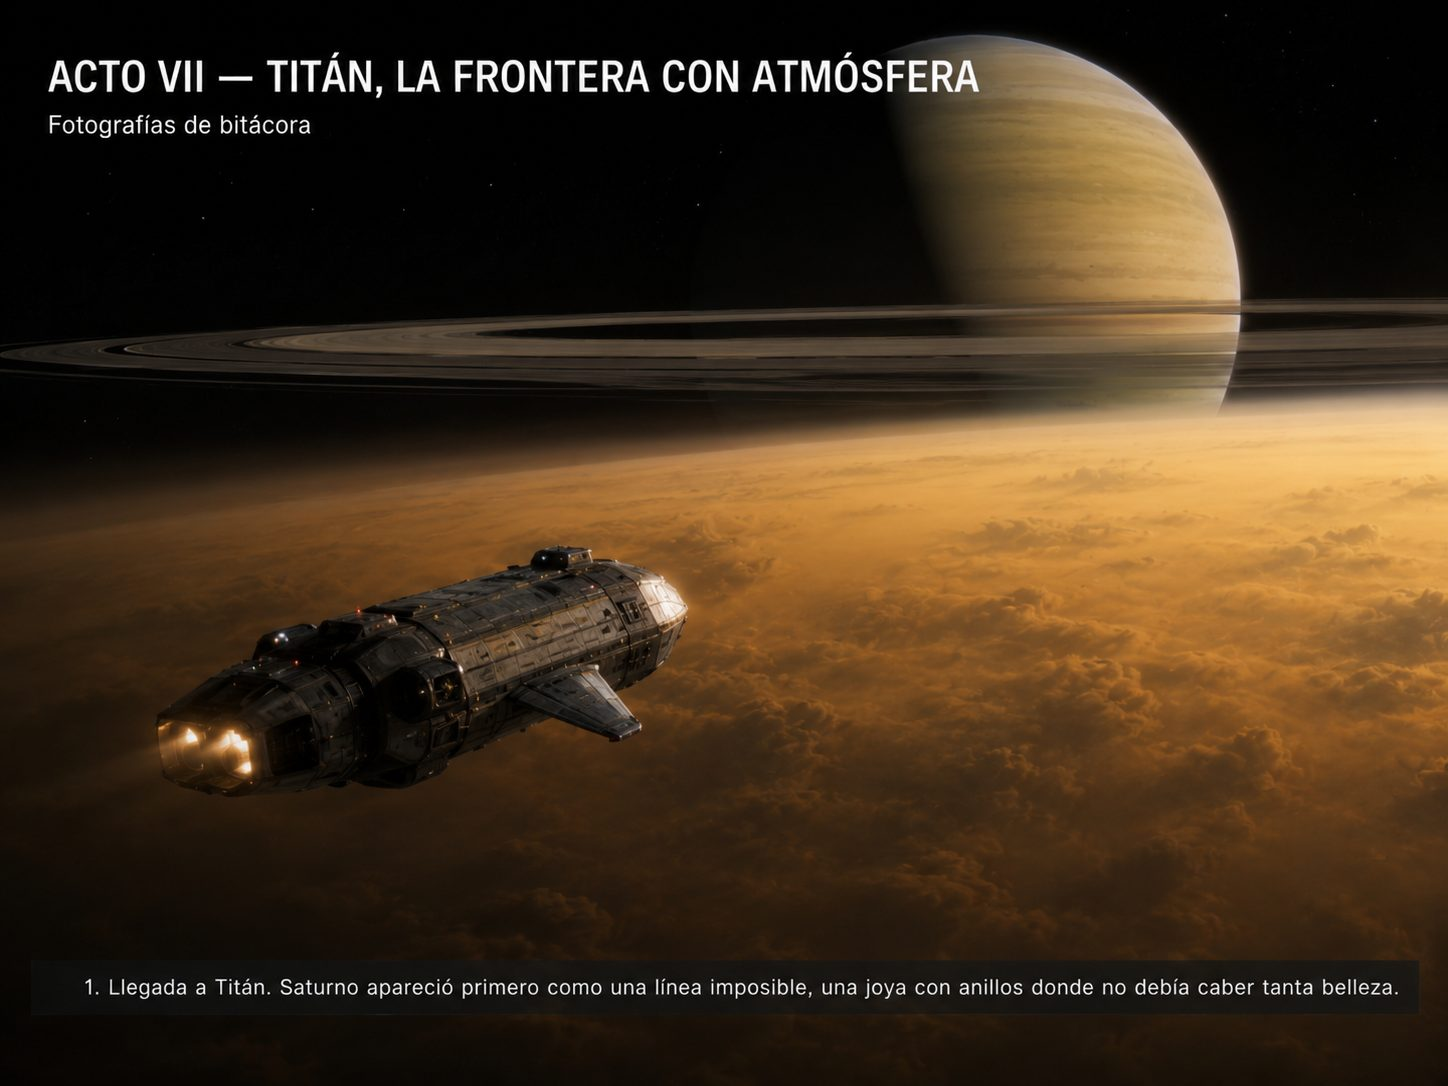
\includegraphics[width=0.9\textwidth]{07_1_llegadaatitnviajeinterplanetario.jpg}
\end{figure}

Llevé media hora mirándolo antes de darme cuenta de que había dejado de tomar notas.

Titán estaba envuelto en naranja.

\begin{figure}[h]
\centering
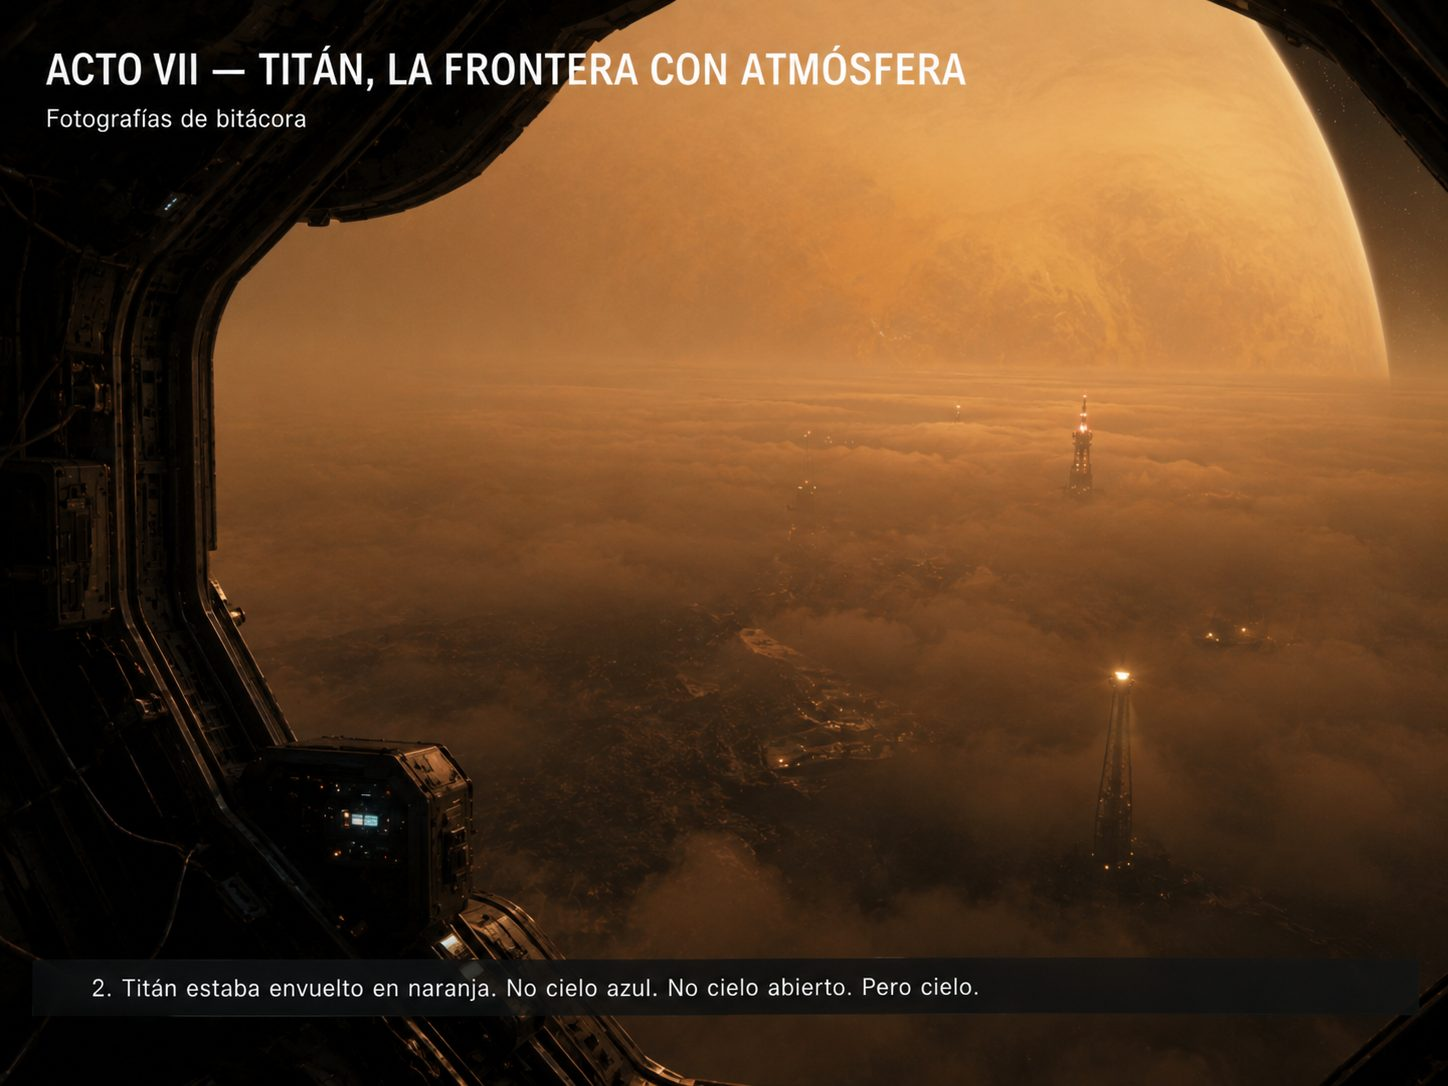
\includegraphics[width=0.9\textwidth]{07_2_vistadesdelanaveentitn.jpg}
\end{figure}

La bruma es lo primero que ves: una capa continua de hazes de nitrógeno y metano que convierte la luna en una esfera opaca. No puedes ver la superficie desde el espacio. Entras a través de ella, y mientras bajas tienes la sensación extraña de que el exterior se vuelve más cercano y a la vez más oscuro. El naranja se oscurece. La densidad del aire cambia. Los sistemas de la lanzadera trabajan diferente aquí que en Marte o en la Luna: hay atmósfera real, presión real, viento real.

La colonia principal no estaba en superficie abierta. Estaba bajo cúpulas bajas, semienterradas, conectadas con puertos aerostáticos.

\begin{figure}[h]
\centering
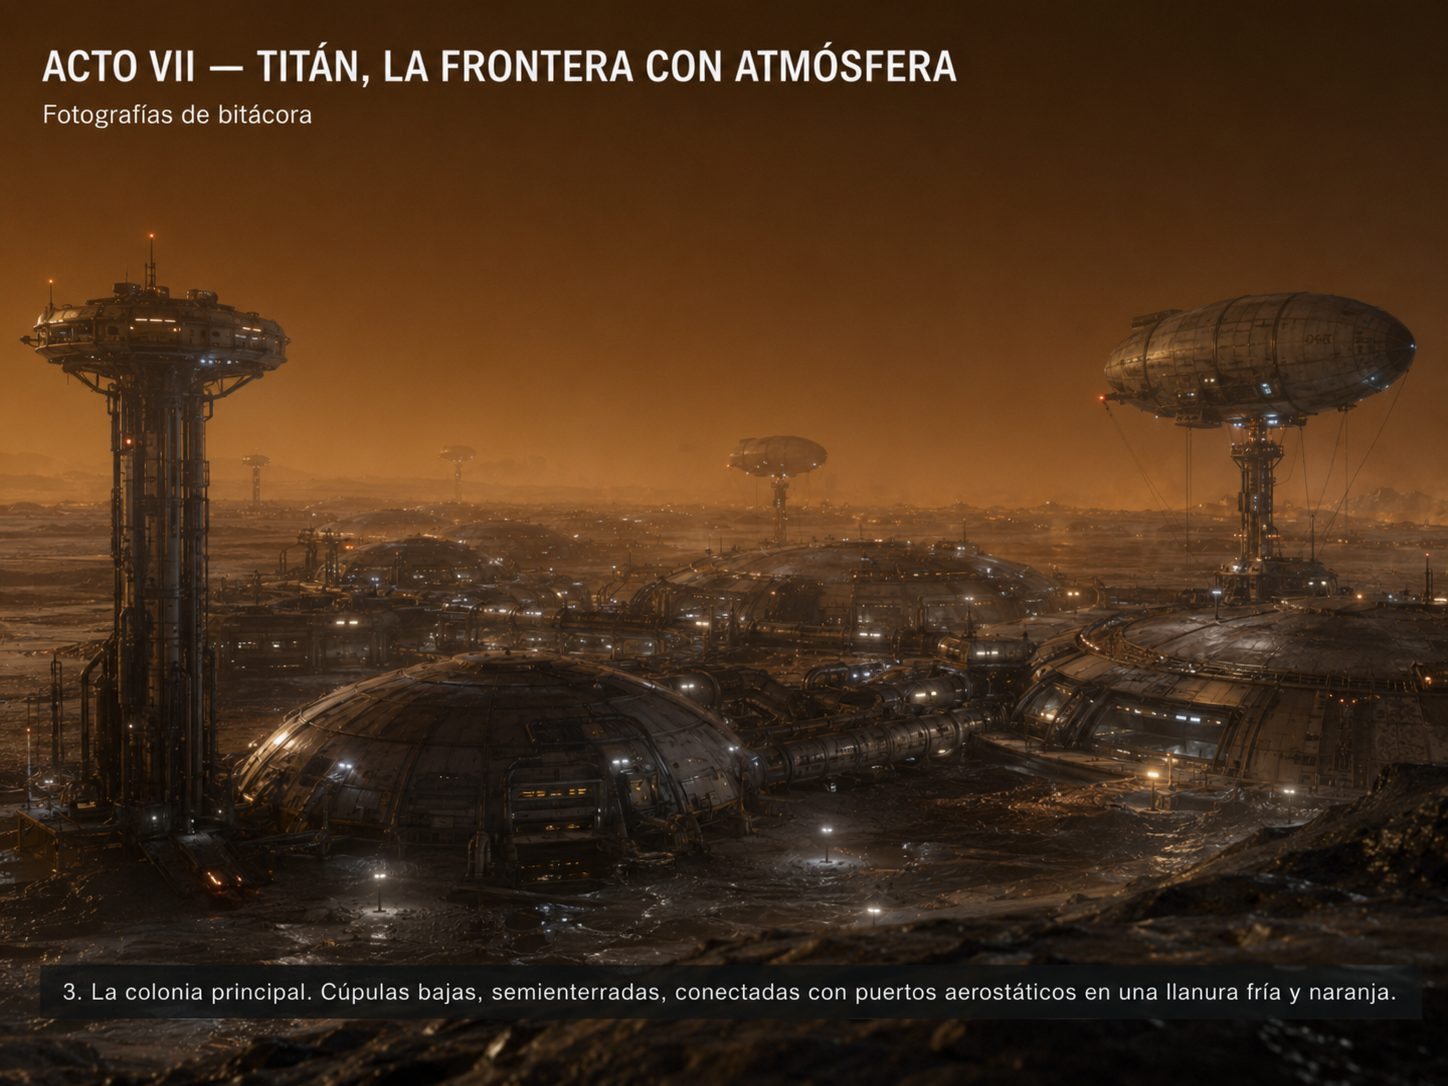
\includegraphics[width=0.9\textwidth]{07_3_coloniaindustrialentitnfuturolejano.jpg}
\end{figure}

Había dirigibles industriales flotando a baja altitud, transportando hidrocarburos, piezas, personal. Eran lentos, enormes y completamente silenciosos vistos desde dentro de la cúpula, como medusas que se hubieran perdido en el cielo equivocado.

\begin{figure}[h]
\centering
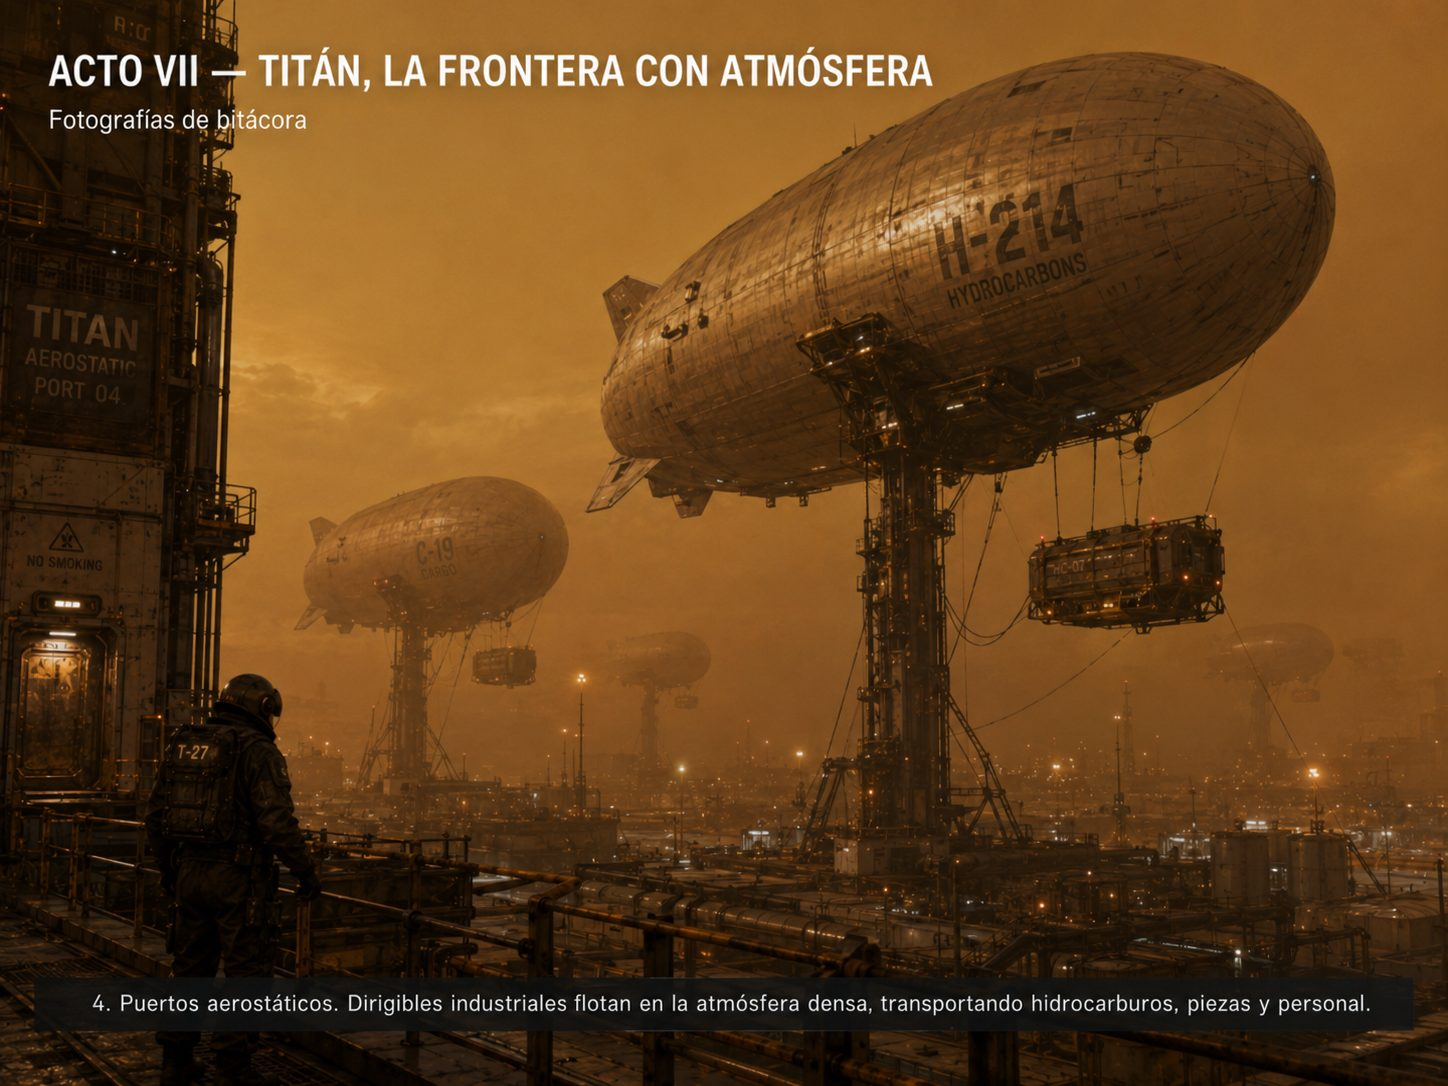
\includegraphics[width=0.9\textwidth]{07_4_puertosaerostticosenunfuturoindustrial.jpg}
\end{figure}

Después de tantos puertos metálicos, Titán parecía casi orgánico.

Frío, tóxico, letal a toda temperatura y presión sin traje, con una química de superficie que haría las delicias de cualquier geólogo alienígena. Pero orgánico. Había algo en la combinación de cielo denso, viento audible contra la cúpula exterior y luz filtrada que lo hacía sentir más vivo que ningún otro lugar del sistema exterior.

\begin{figure}[h]
\centering
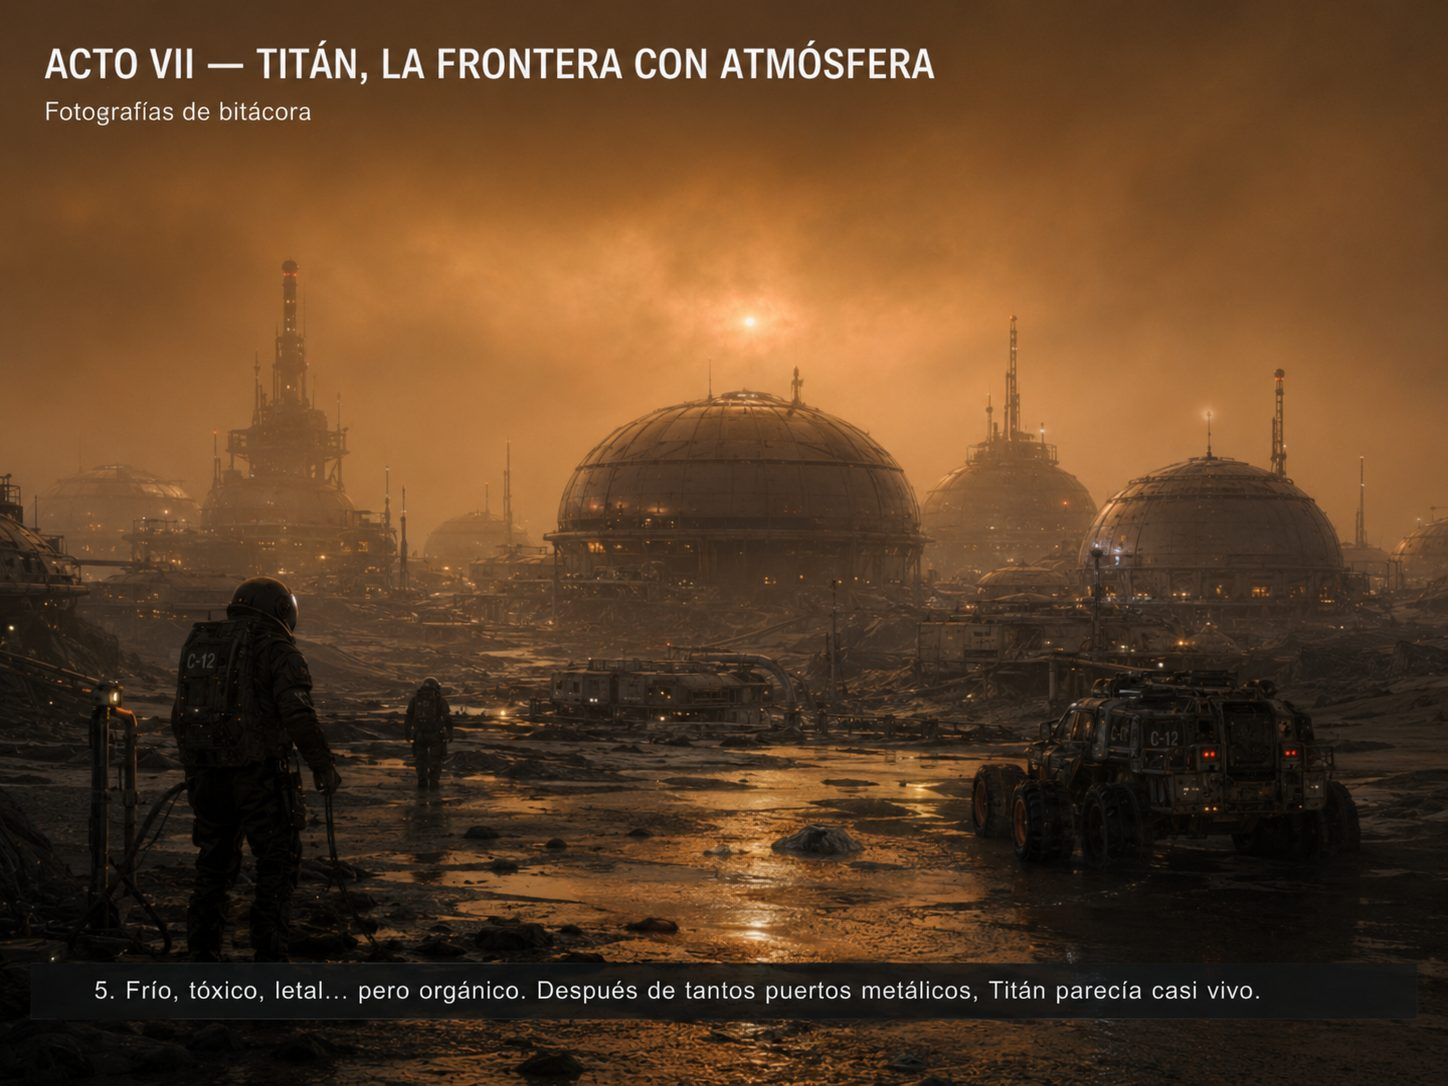
\includegraphics[width=0.9\textwidth]{07_5_titnfronteraindustrialenlaniebla.jpg}
\end{figure}

Allí se fabricaban polímeros, combustibles, blindajes y compuestos que alimentaban media infraestructura exterior. La estación entre Júpiter y Saturno dependía de Titán más de lo que los comunicados oficiales admitían. En los pasillos de la instalación industrial había carteles de producción con números que no terminé de entender, pero cuyo tamaño era suficientemente claro.

Titán no era el destino de nadie. Era el lugar donde se fabricaba todo lo demás.

Un técnico que me acompañó por las instalaciones me mostró la sección de polímeros de alta presión. Señaló una tubería del grosor de un edificio.

—Eso va a La Exterior —dijo—. Para los radiadores de la matriz. Titanio-polímero reforzado. Solo se puede fabricar aquí porque necesitas la temperatura y la presión atmosférica de Titán para conseguir la densidad correcta.

—¿Y cuánto tiempo llevan enviando material?

—Desde que La Exterior existe. Antes también, cuando era otra cosa.

Caminé de vuelta a la cúpula de habitación con eso dando vueltas. Titán llevaba décadas alimentando algo que no veía. Construyendo piezas de una máquina cuyo tamaño completo no podría ver nunca desde aquí.

\begin{figure}[h]
\centering
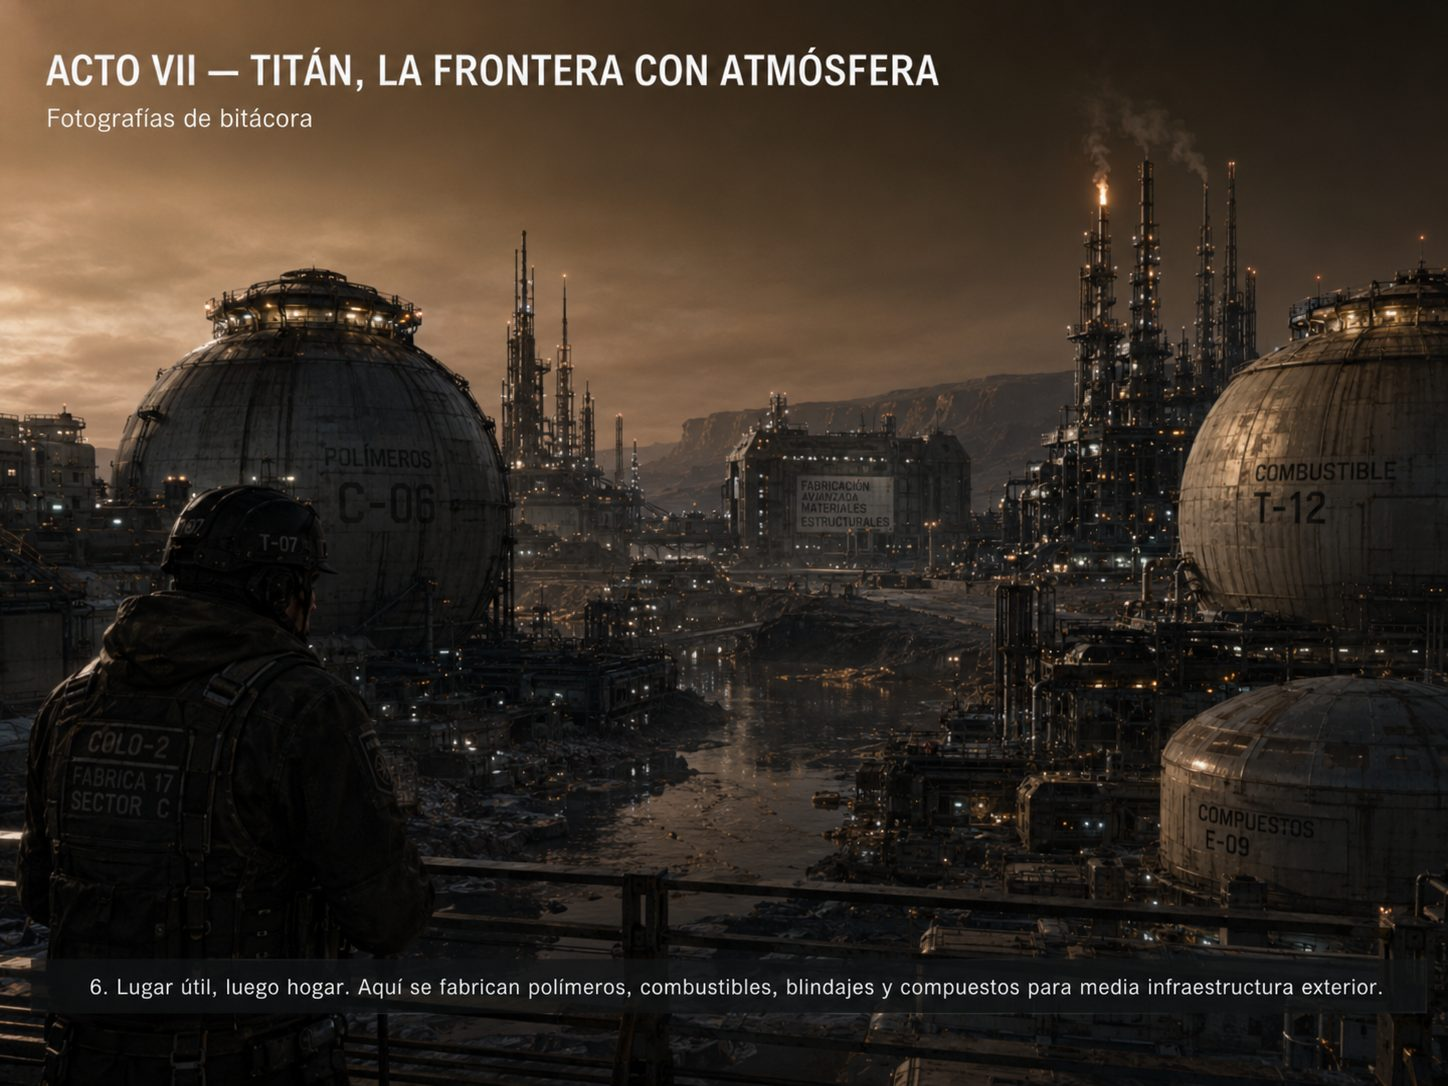
\includegraphics[width=0.9\textwidth]{07_6_coloniaindustrialentitanalanochecer.jpg}
\end{figure}

Esa noche, en mi diario, escribí:

> La civilización no avanza desde los lugares hermosos. Avanza desde los lugares útiles. Luego aprende a llamarlos hogar.

\vspace{1.5em}
\begin{center}$\ast$\quad$\ast$\quad$\ast$\end{center}
\vspace{1.5em}

\chapter*{Acto VIII — La Gran Estación Warp Exterior}
\addcontentsline{toc}{chapter}{Acto VIII — La Gran Estación Warp Exterior}
\markboth{Acto VIII — La Gran Estación Warp Exterior}{Acto VIII — La Gran Estación Warp Exterior}

*\textit{Días 84–100. La Exterior. Región entre Júpiter y Saturno.}*

La llamaban simplemente *\textit{La Exterior}*.

No estaba exactamente a medio camino entre Júpiter y Saturno, porque nada en el sistema solar permanece quieto. Era un complejo de trayectoria propia, mantenido en una región relativamente limpia y vigilada, lejos de lunas, anillos, rutas comerciales densas y pozos gravitatorios peligrosos. Una zona donde el espacio era, en la medida de lo posible, predecible.

Desde lejos parecía una constelación artificial.

\begin{figure}[h]
\centering
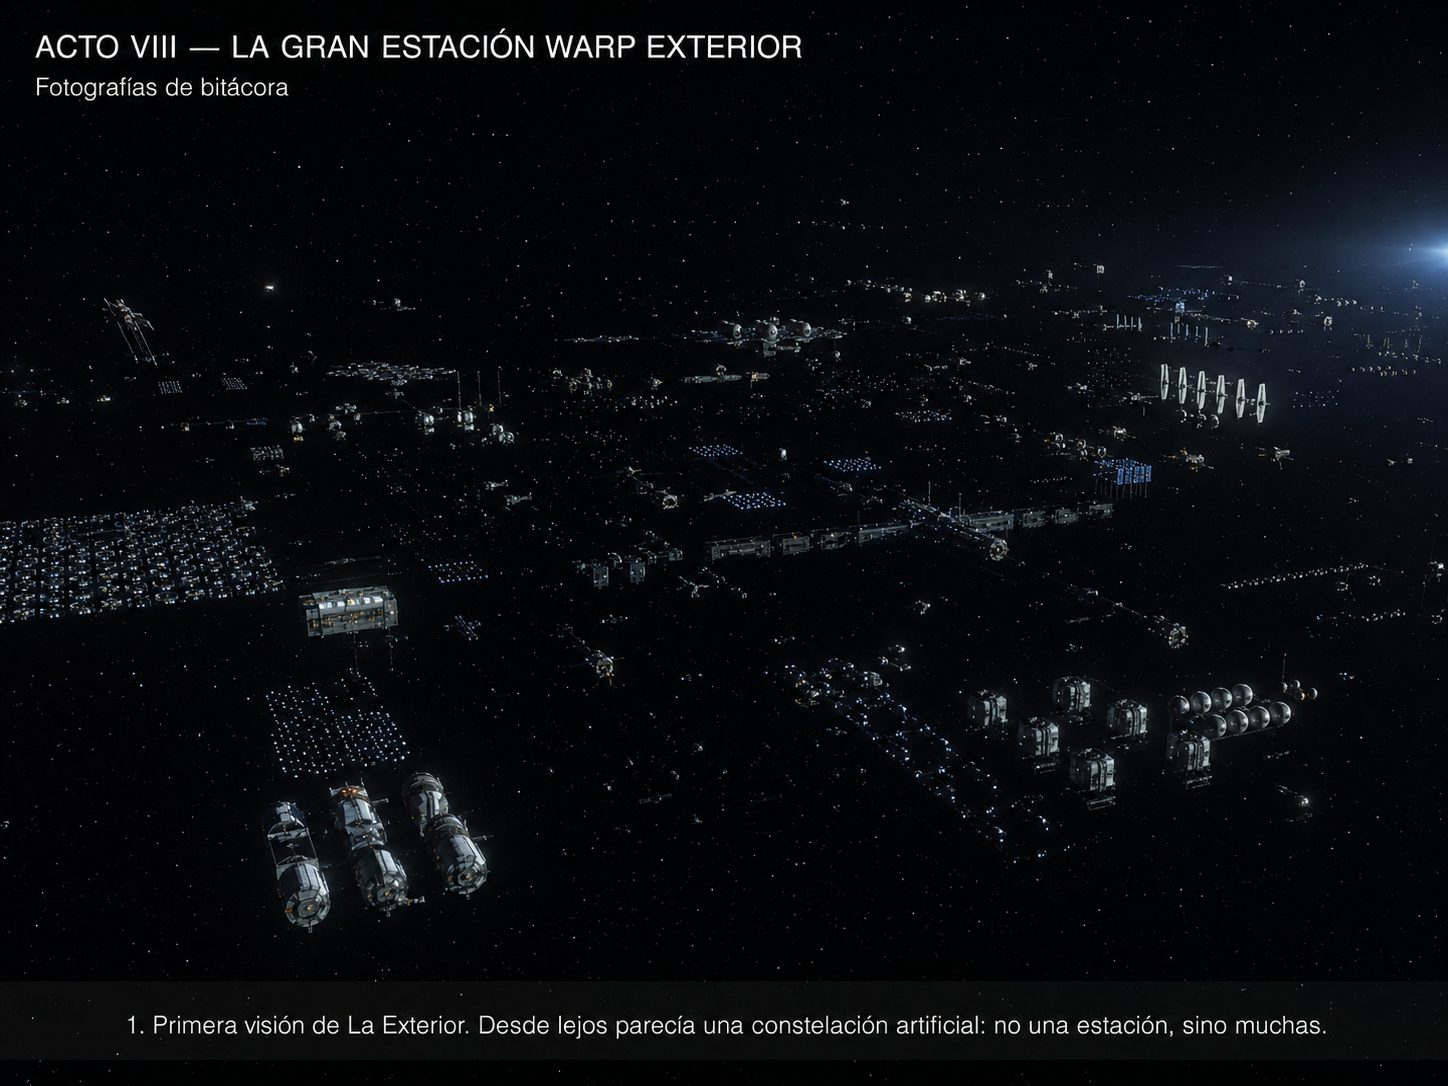
\includegraphics[width=0.9\textwidth]{08_1_lagranestacinwarpexterior.jpg}
\end{figure}

El primer avistamiento fue en los sensores: una región de calor anómalo, demasiado ordenado para ser natural. Luego, en el visor óptico, puntos de luz que no parpadeaban porque no eran estrellas. Finalmente, al aproximarnos durante horas, la escala empezó a revelarse capa a capa, como una ciudad que ves acercándote en coche y que resulta ser tres veces más grande de lo que calculabas.

No era una estación sino muchas: hábitats conectados por túneles pressurizados, astilleros donde la actividad de drones era constante y organizada, depósitos de masa con la geometría de edificios flotantes, reactores con sus radiadores desplegados como flores de metal frío, enjambres de espejos de seguimiento solar para alimentación energética, almacenes de hielo del tamaño de bloques de viviendas, fábricas de campo donde se fabricaban los componentes más delicados de la maquinaria warp. Y muelles de cuarentena, separados del resto, para naves que llegaban de rutas no certificadas.

\begin{figure}[h]
\centering
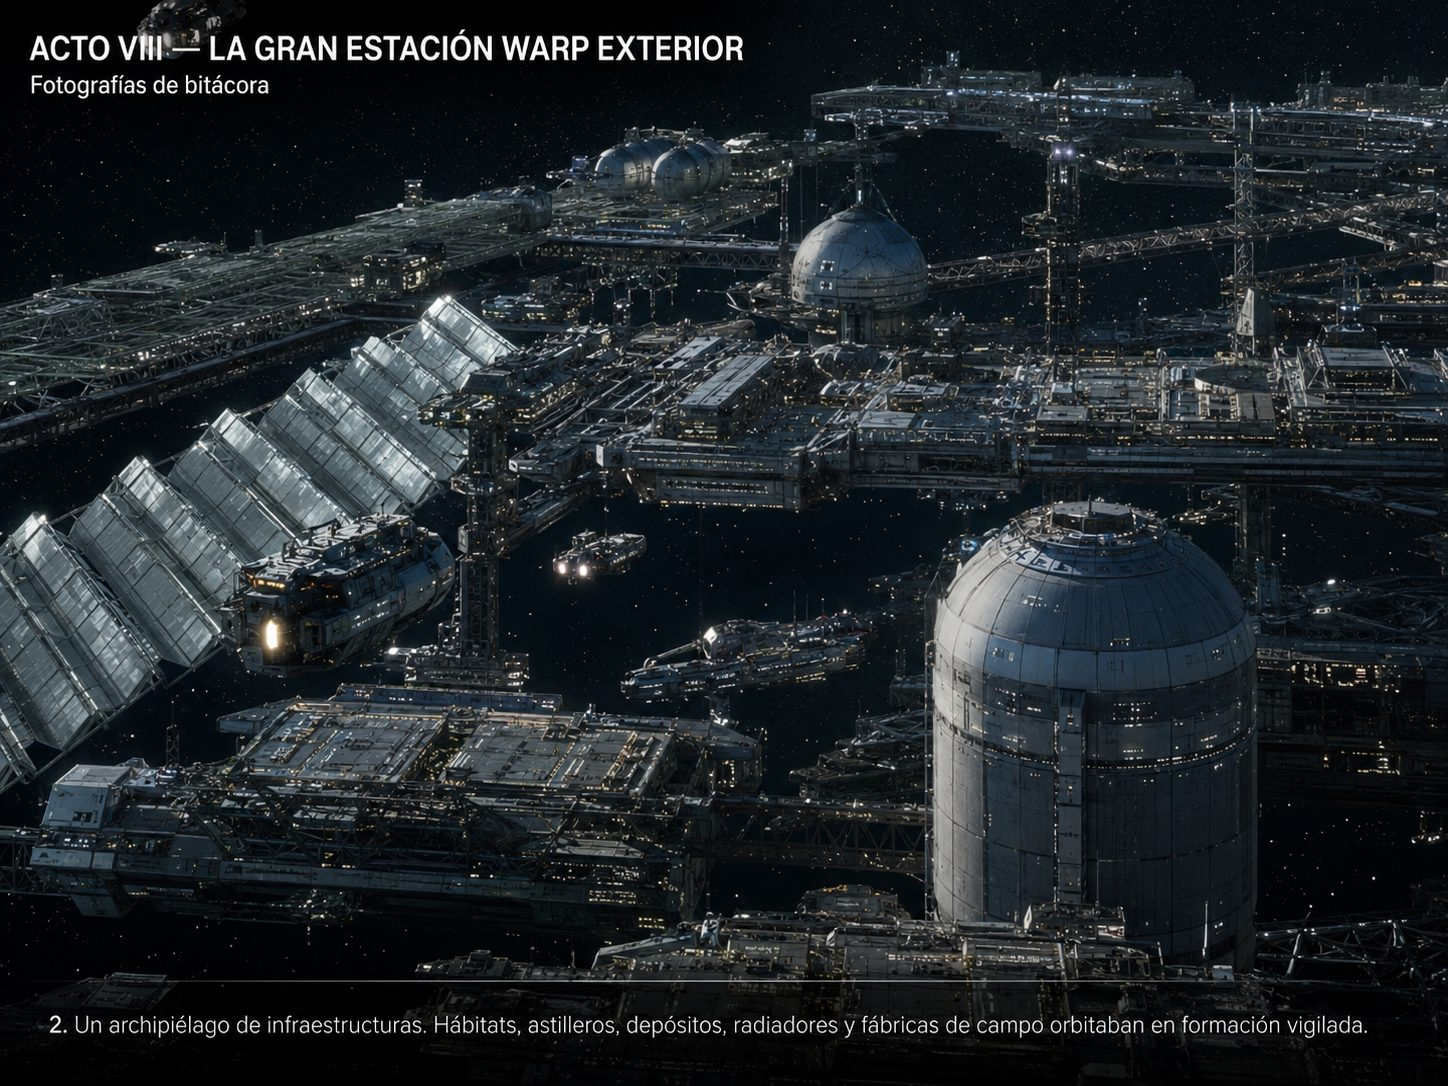
\includegraphics[width=0.9\textwidth]{08_2_estacinwarpenelvacoespacial.jpg}
\end{figure}

Separada de todo lo vivo por miles de kilómetros de vacío vigilado, la *\textit{Matriz de Lanzamiento Interestelar}*.

La matriz era la cosa más grande que he visto jamás.

Una línea de anillos. No uno. Decenas.

\begin{figure}[h]
\centering
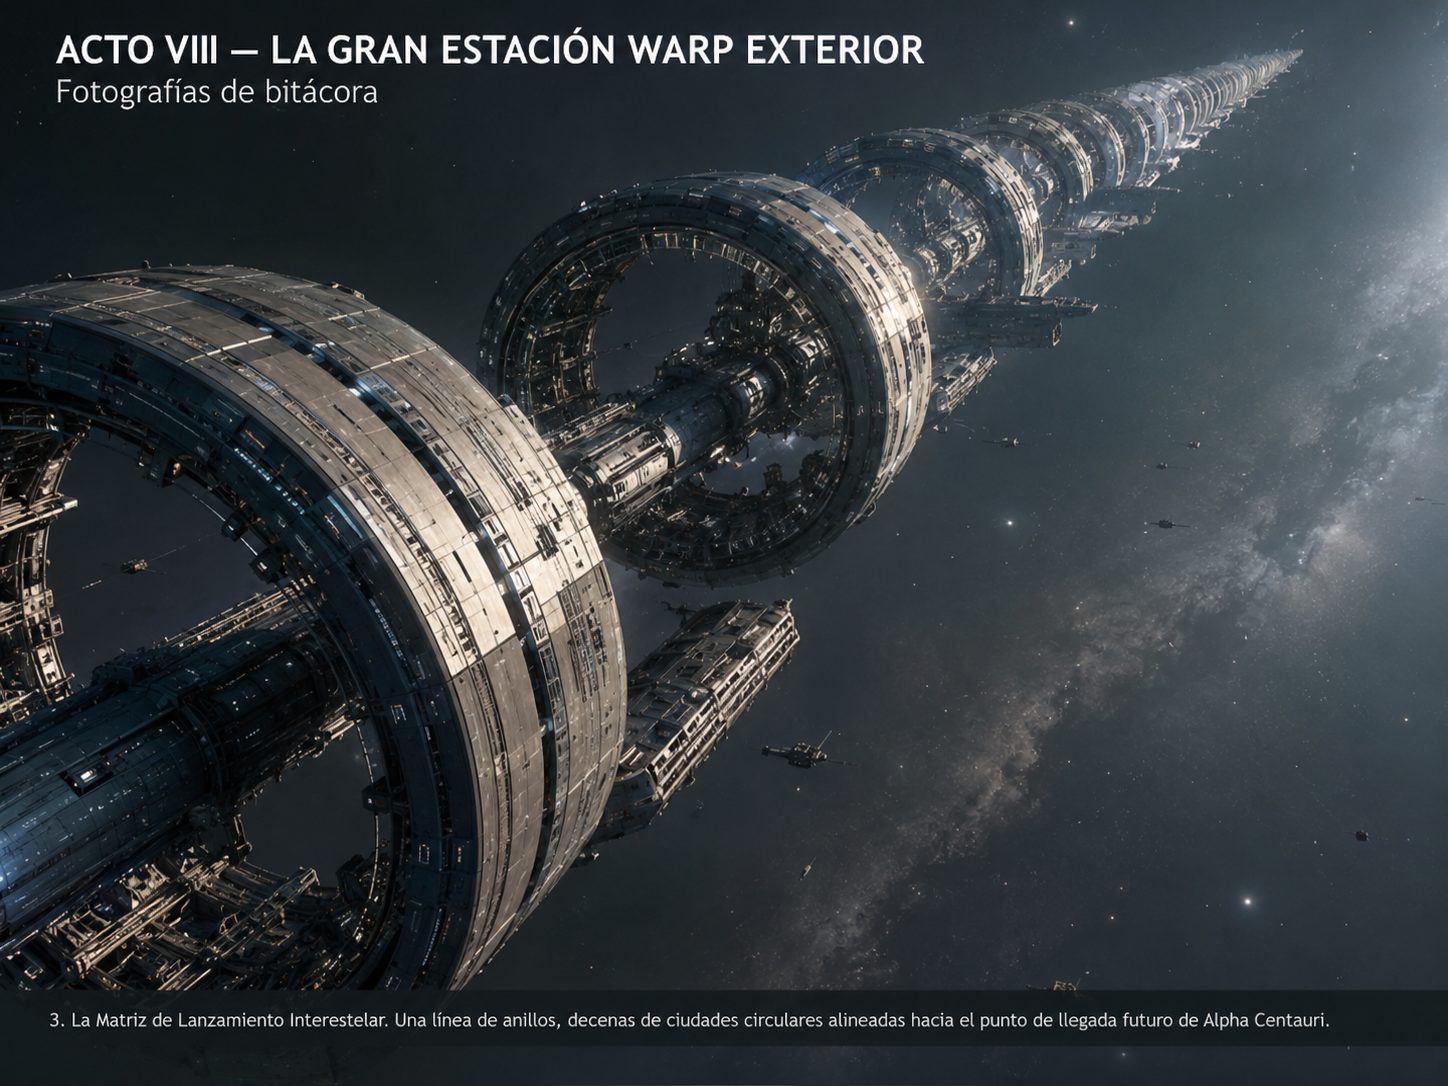
\includegraphics[width=0.9\textwidth]{08_3_laestacinwarpenelespacio.jpg}
\end{figure}

Cada anillo era una ciudad circular de metal y vacío, con sus propios sistemas de refrigeración, sus propias balizas de alineación, su propio enjambre de drones de mantenimiento. Alineados con los demás sobre un eje que no apuntaba hacia donde Alpha Centauri estaba, sino hacia donde Alpha Centauri estaría cuando la nave llegara. Un cálculo que incorporaba el movimiento estelar durante el tiempo de viaje, calculado y recalculado con años de antelación.

El cicler interestelar esperaba acoplado al primer tramo.

Se llamaba *\textit{Atenea Larga}*.

Eleven kilómetros de estructura principal. Tres hábitats rotatorios con gravedad simulada de 0,4g. Escudo frontal de hielo y grafeno de casi medio kilómetro de superficie efectiva. Reactores de fusión en racimo, cuatro parejas. Bancos superconductores. Anillos de curvatura propios, más grandes que cualquier cosa que hubiera visto en los ciclers del sistema solar interior. Capacidad para ocho mil pasajeros y treinta mil embriones criopreservados de especies terrestres.

\begin{figure}[h]
\centering
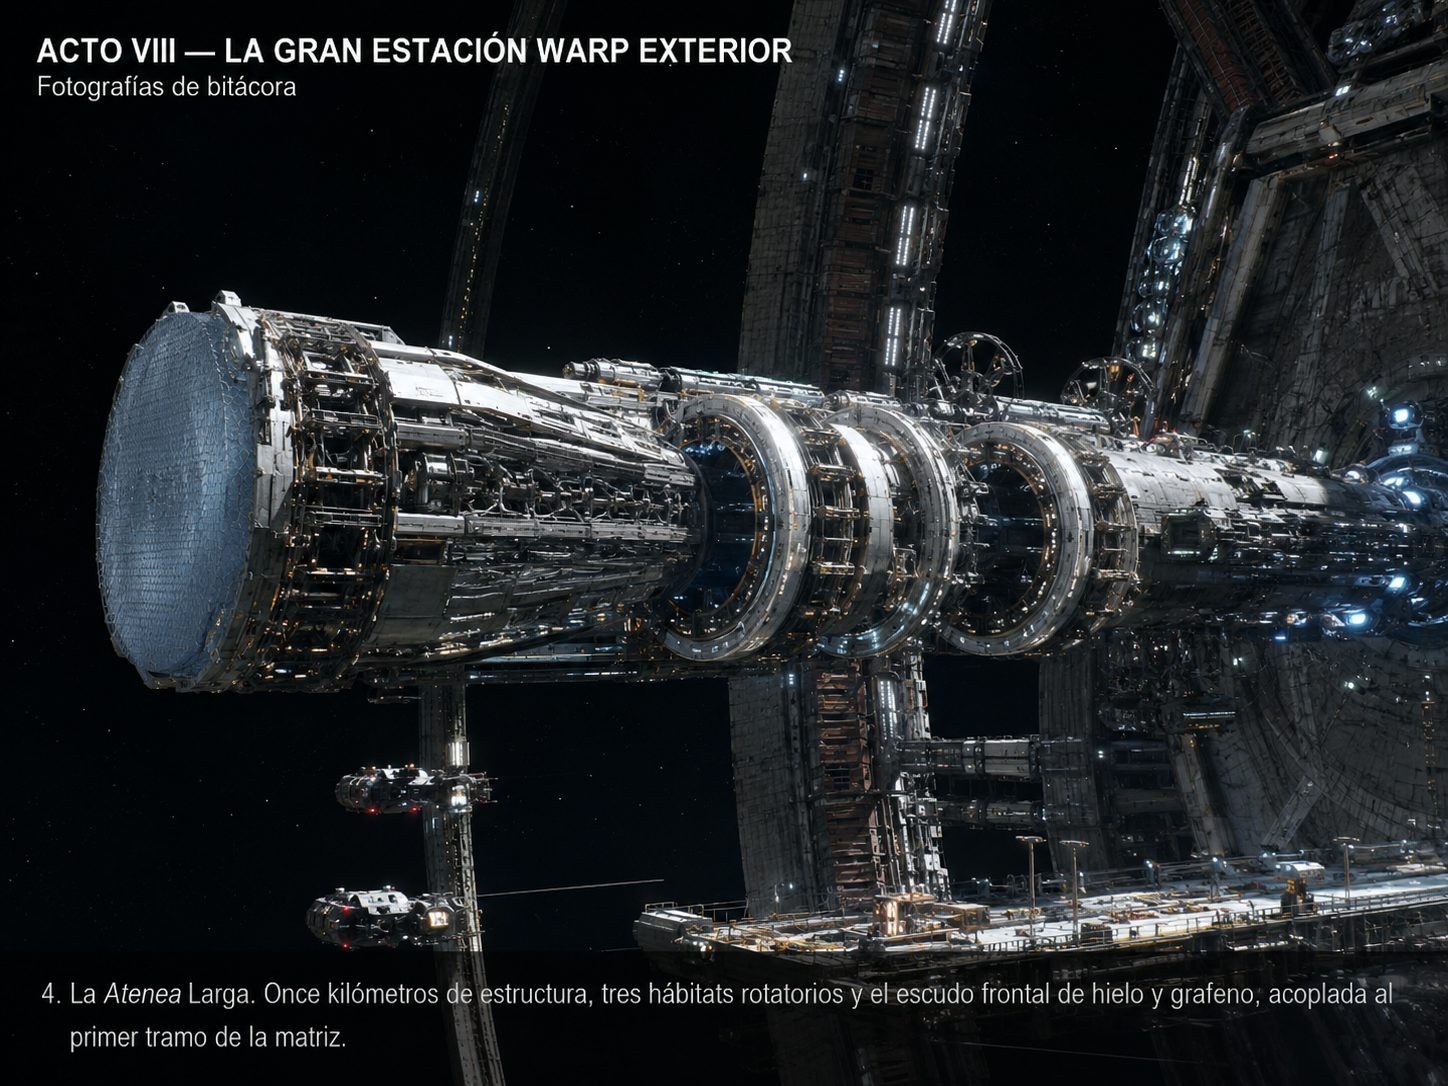
\includegraphics[width=0.9\textwidth]{08_4_estacinorbitalyhbitatsrotatorios.jpg}
\end{figure}

Pero lo más importante era lo que no podía hacer sola.

Sola, la Atenea Larga podía alcanzar 1,3c en crucero estable. Bastante para el regreso, cuando no habría catapulta equivalente en Alpha Centauri. Con la matriz, podía salir a 4,7c efectivos.

La ida duraría un año.

La vuelta, si algún día volvía, más de tres.

Aquello cambiaba psicológicamente el viaje. Un año todavía pertenecía a la escala humana, la escala de los embarazos y las cosechas y los contratos laborales. Tres o cuatro ya eran historia. Tres o cuatro años eran el tiempo que tardó alguien en conquistar un continente, en fundar una ciudad, en cambiar un mundo.

Durante la semana previa al lanzamiento, la estación entera vibró con preparativos. No vibración física —todo aquí era demasiado grande para vibrar de esa manera—, sino social. Todo el mundo sabía que algo enorme iba a ocurrir. En los corredores se hablaba más bajo, con ese respeto involuntario que da la presencia de algo mayor que uno mismo. En los observatorios había listas de espera de cuatro horas. Los niños de La Exterior recibieron el día libre sin que nadie explicara por qué.

\begin{figure}[h]
\centering
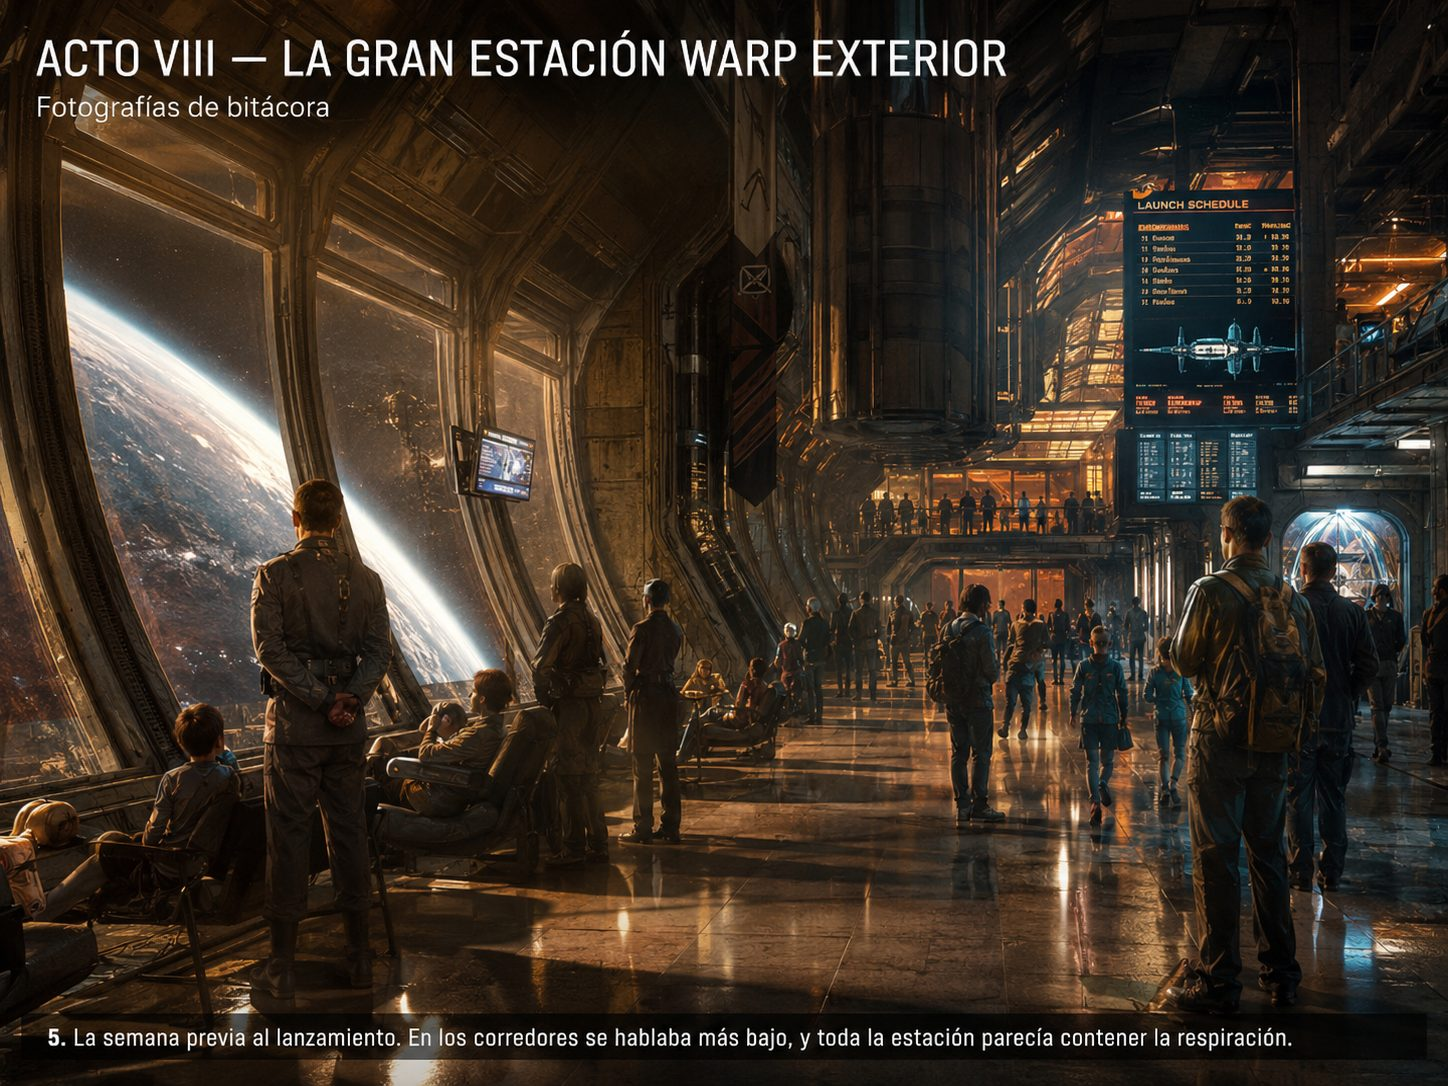
\includegraphics[width=0.9\textwidth]{08_5_lagranestacinwarpexteriorzonadeviajeros.jpg}
\end{figure}

Yo pasé la última noche mirando la matriz desde un ventanal blindado de la zona civil.

Estaba encendida a baja intensidad para las pruebas de sincronización: los anillos con un brillo frío y regular, los haces de alineación azulados, los radiadores oscuros en el fondo. Desde el ventanal parecía una escritura en un idioma que no termino de aprender.

No parecía una puerta.

Parecía una pregunta.

\begin{figure}[h]
\centering
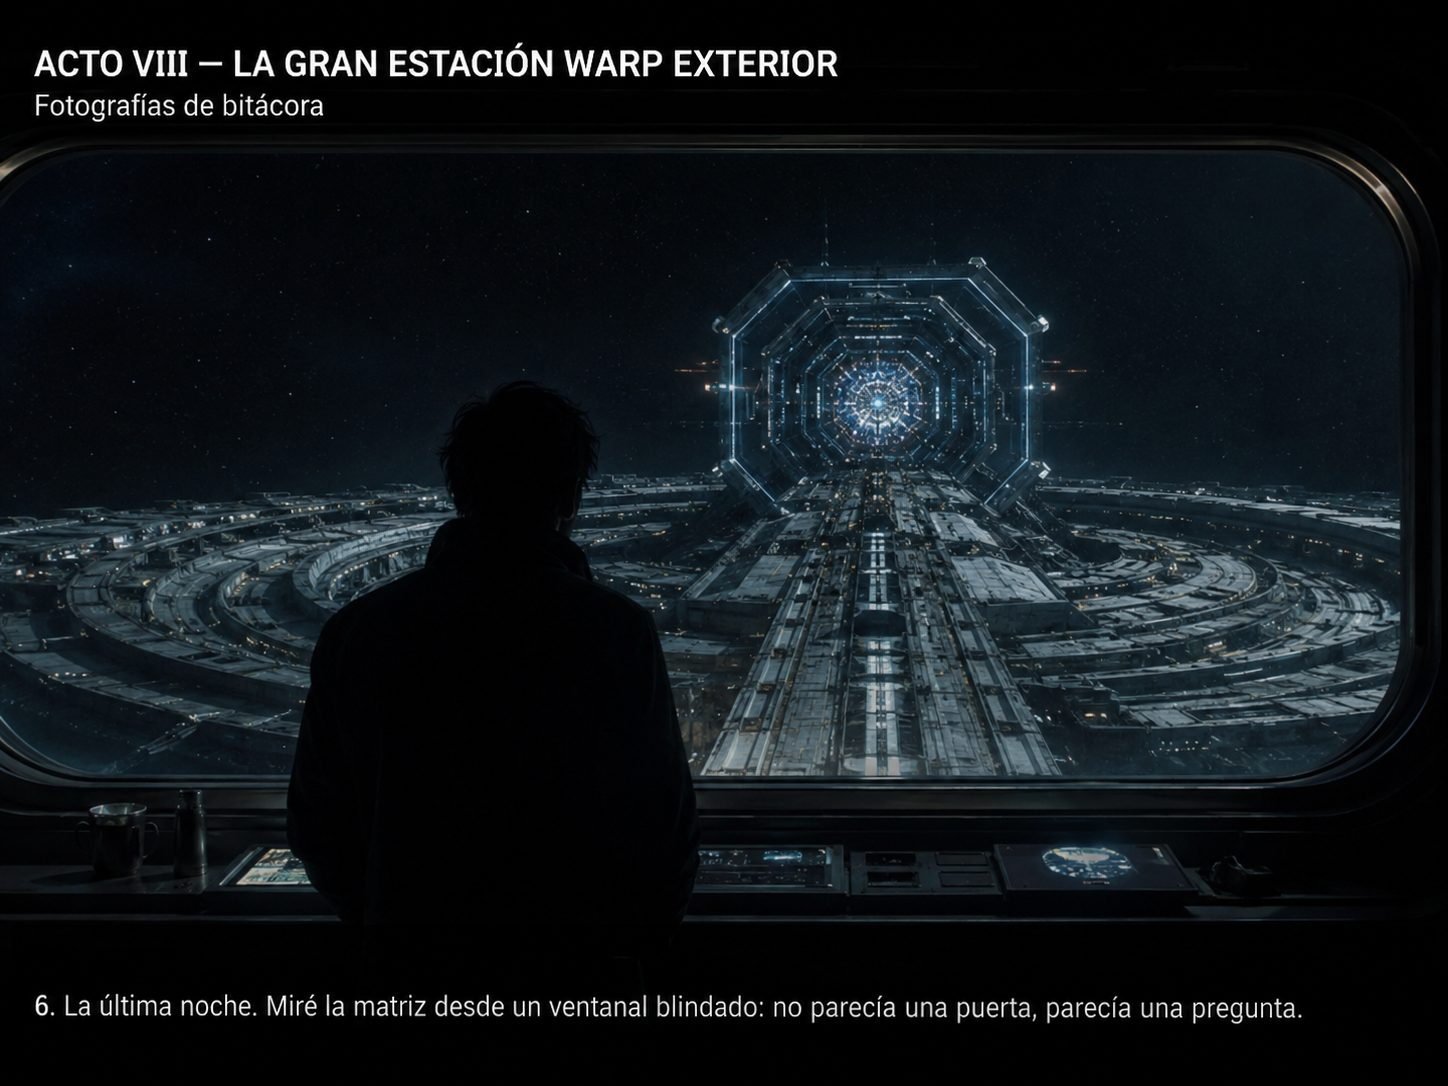
\includegraphics[width=0.9\textwidth]{08_6_nocheenlaestacinwarp.jpg}
\end{figure}

\vspace{1.5em}
\begin{center}$\ast$\quad$\ast$\quad$\ast$\end{center}
\vspace{1.5em}

\chapter*{Acto IX — Lanzamiento}
\addcontentsline{toc}{chapter}{Acto IX — Lanzamiento}
\markboth{Acto IX — Lanzamiento}{Acto IX — Lanzamiento}

*\textit{Día 101. Atenea Larga. Matriz de Lanzamiento Interestelar. 04:12 hora estándar.}*

El embarque en la Atenea Larga duró diecisiete horas.

Diecisiete horas para mover ocho mil personas desde los módulos de espera de La Exterior hasta sus camarotes, sus puestos de trabajo o sus secciones de criopreservación. El proceso tenía la solemnidad de una mudanza enorme, no la de una ceremonia. Había colas en las esclusas. Había familias buscando su módulo con mapas en la pantalla. Había técnicos revisando listas en tabletas y señalando pasillos sin mirar a los pasajeros.

No hubo música solemne. No hubo discursos grandiosos hasta el final, y fueron breves. Dos minutos del director de misión, noventa segundos de la capitana. Palabras sobre lo que representaba esto, sobre las generaciones que habían trabajado para que fuera posible. Correcto, apropiado, y rápidamente olvidado por la urgencia de todo lo que había que hacer aún.

La solemnidad verdadera estaba en los gestos pequeños.

Una madre ajustando el cuello del traje de su hijo antes de que cruzara la esclusa hacia la sección de tripulación. Un técnico que pasó la mano lentamente por la pared del corredor de mantenimiento antes de cerrar la escotilla, como quien se despide de una habitación. Dos ancianos mirando juntos, en silencio, una grabación de lluvia terrestre en una pantalla pequeña: el sonido del agua cayendo sobre asfalto, que desde aquí sonaba a otra especie de música.

\begin{figure}[h]
\centering
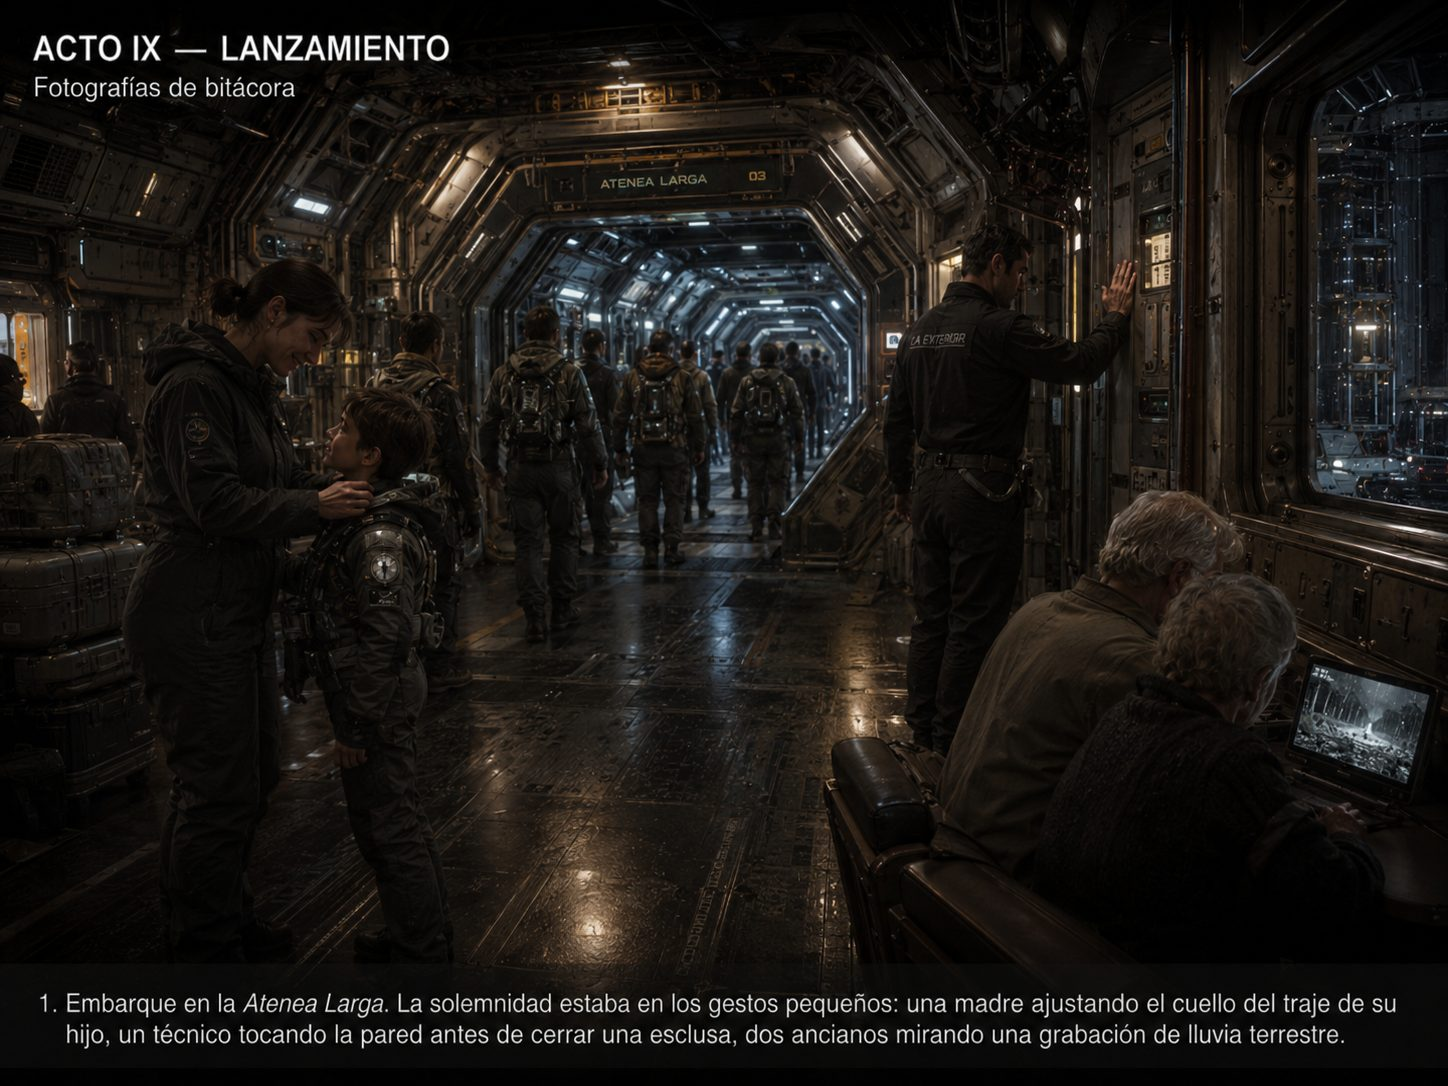
\includegraphics[width=0.9\textwidth]{09_1_embarqueenlaatenealarga.jpg}
\end{figure}

Mi camarote era estrecho, con el ancho justo para el catre y el armario, pero tenía una pantalla de cuarenta centímetros con vista exterior continua. Coloqué la grabadora sobre la repisa y la encendí. Luego la apagué. Luego la volví a encender. Decidí que lo que iba a pasar se merecía escucharse en silencio.

\begin{figure}[h]
\centering
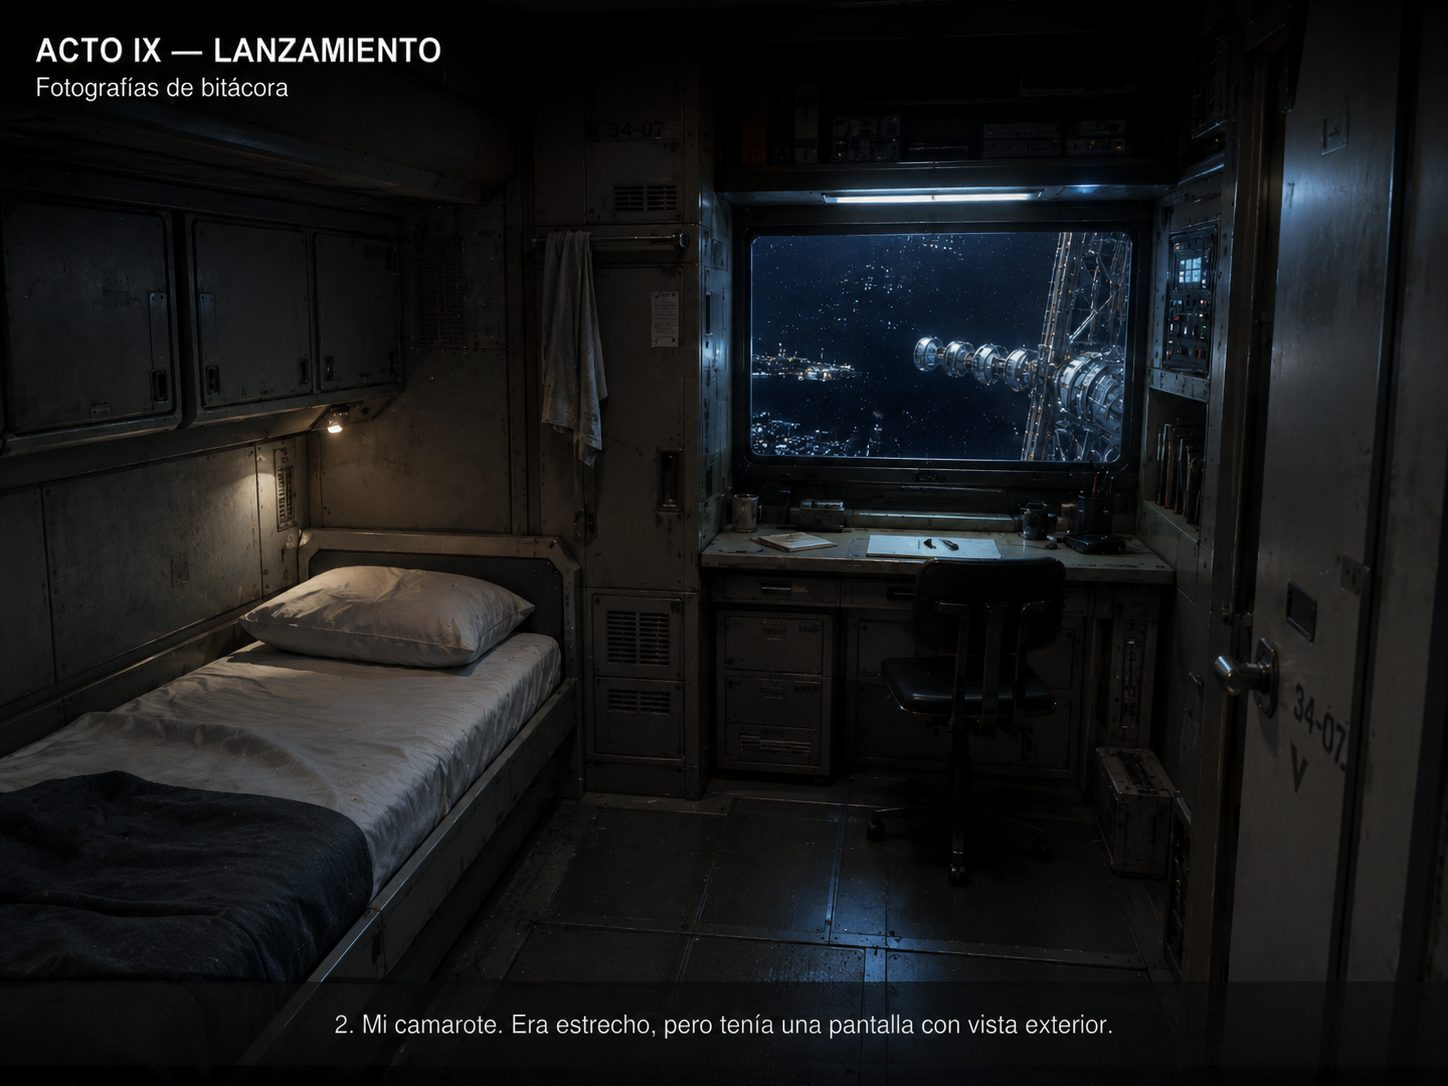
\includegraphics[width=0.9\textwidth]{09_2_camaroteenestacinespacial.jpg}
\end{figure}

A las 04:12 hora estándar, nos desacoplamos.

La Atenea Larga avanzó lentamente hacia el eje de la matriz.

\begin{figure}[h]
\centering
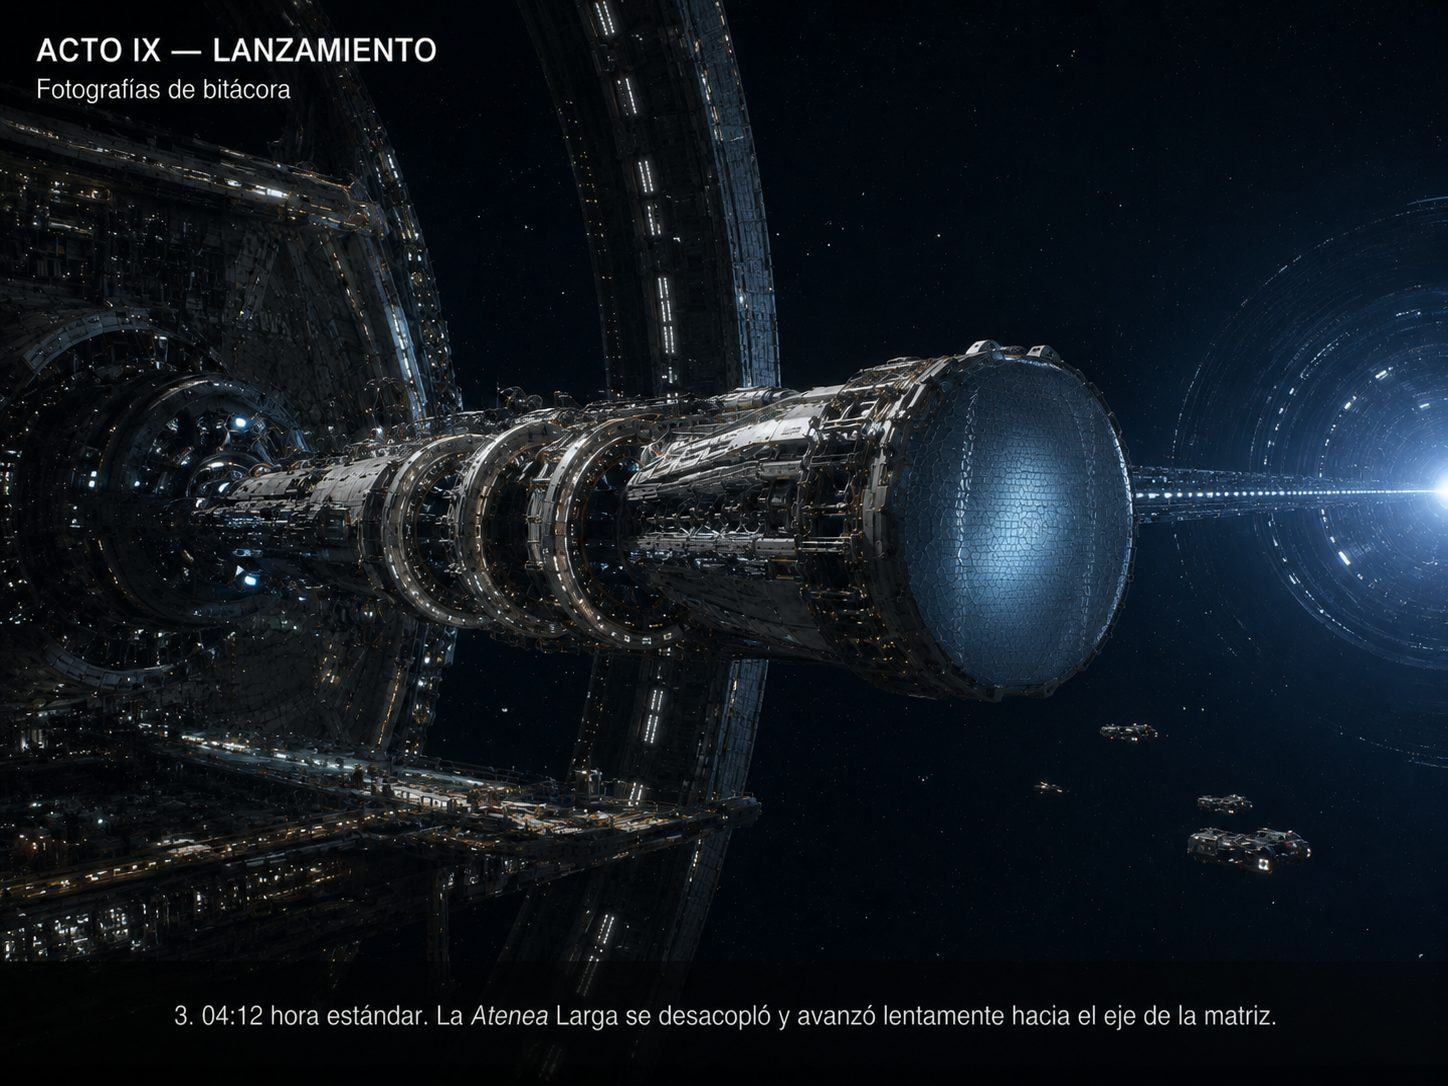
\includegraphics[width=0.9\textwidth]{09_3_lanzamientoenlaestacinespacial.jpg}
\end{figure}

Desde la pantalla veía los anillos a ambos lados, encendiéndose uno tras otro a medida que la nave avanzaba. No con una luz fantástica, sino con líneas frías, blancas y azules, como instrumentos quirúrgicos preparándose para una operación de precisión. El haz de alineación era perfecto. Todo era perfecto. Era el resultado de décadas de ingeniería que habían aprendido a no dejar espacio para lo imprevisto.

\begin{figure}[h]
\centering
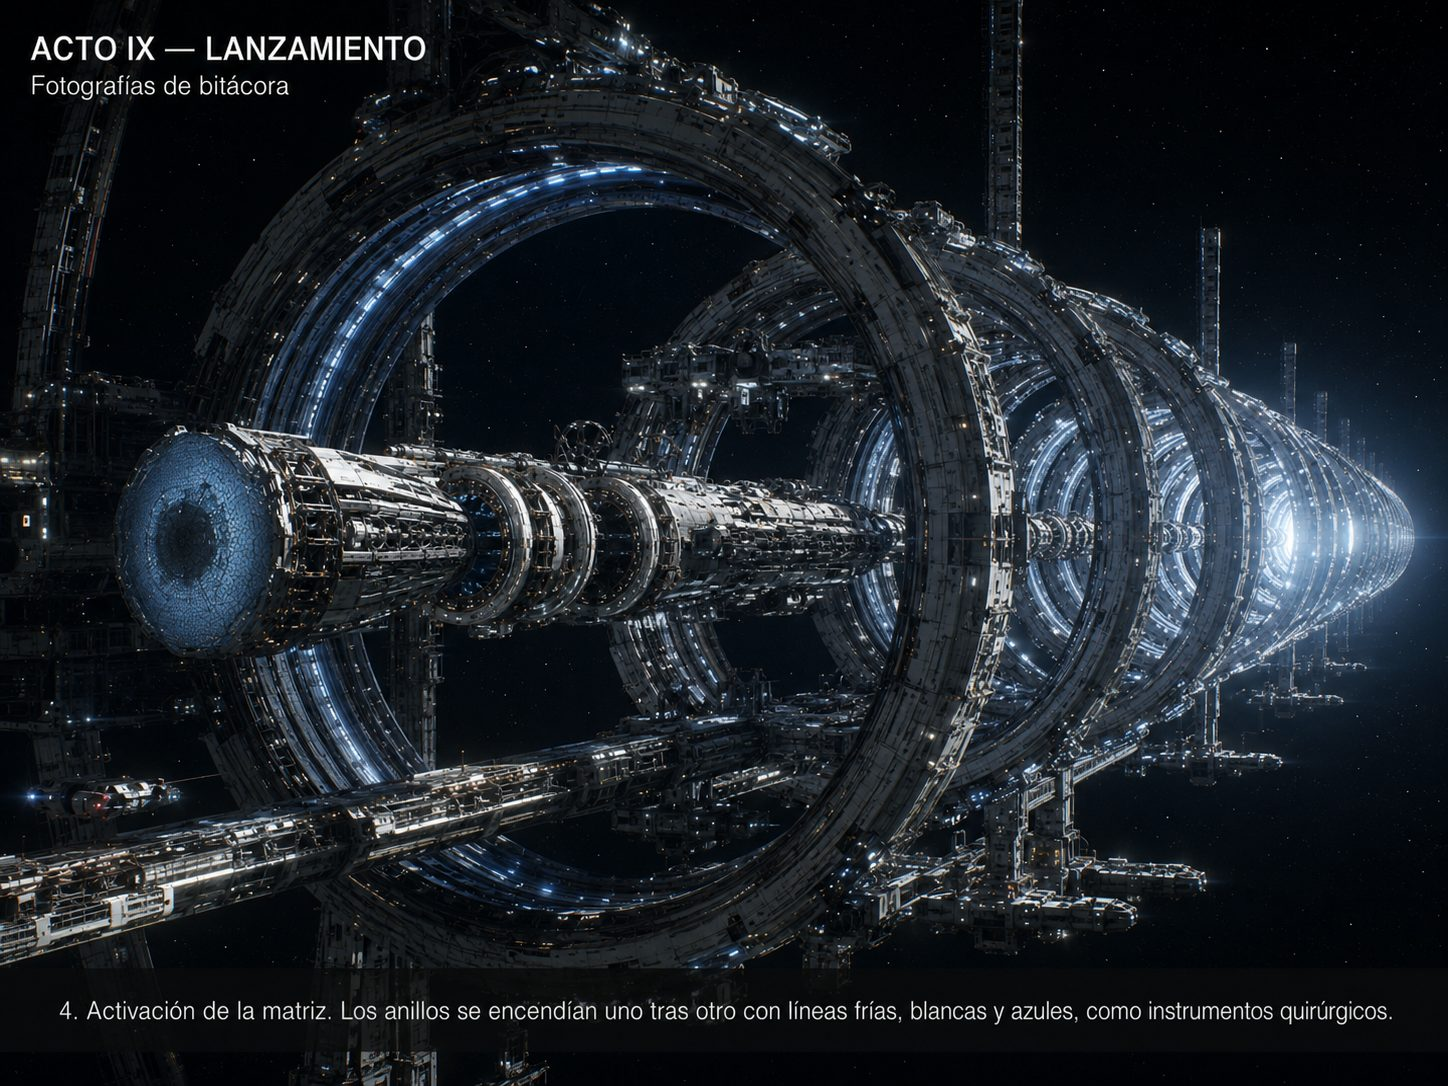
\includegraphics[width=0.9\textwidth]{09_4_estacinespacialylanzamientofuturista.jpg}
\end{figure}

La voz de control llegó por todos los canales simultáneamente. Plana. Precisa. Sin énfasis dramático:

—Matriz uno, sincronizada.
—Matriz dos, sincronizada.
—Vacío polarizado estable.
—Gradiente métrico dentro de tolerancia.
—Corredor Centauri abierto.
—Atenea Larga, autorización de salida.

El capitán respondió:

—Atenea Larga confirma. Nos vemos al otro lado del año.

No hubo empuje.

Ese fue el detalle que nunca olvidaré.

Esperaba fuerza, ruido, algún indicio físico de que una estación entera estaba arrojándonos hacia otra estrella. Esperaba sentir algo que correspondiera a la magnitud del evento. Pero el campo tomó la aceleración y la repartió por la burbuja métrica de manera uniforme. No hubo gradiente inercial. Solo sentí un leve cambio en el oído interno, como cuando un ascensor empieza a moverse muy despacio y la diferencia entre estar quieto y estar en movimiento desaparece en la incertidumbre.

\begin{figure}[h]
\centering
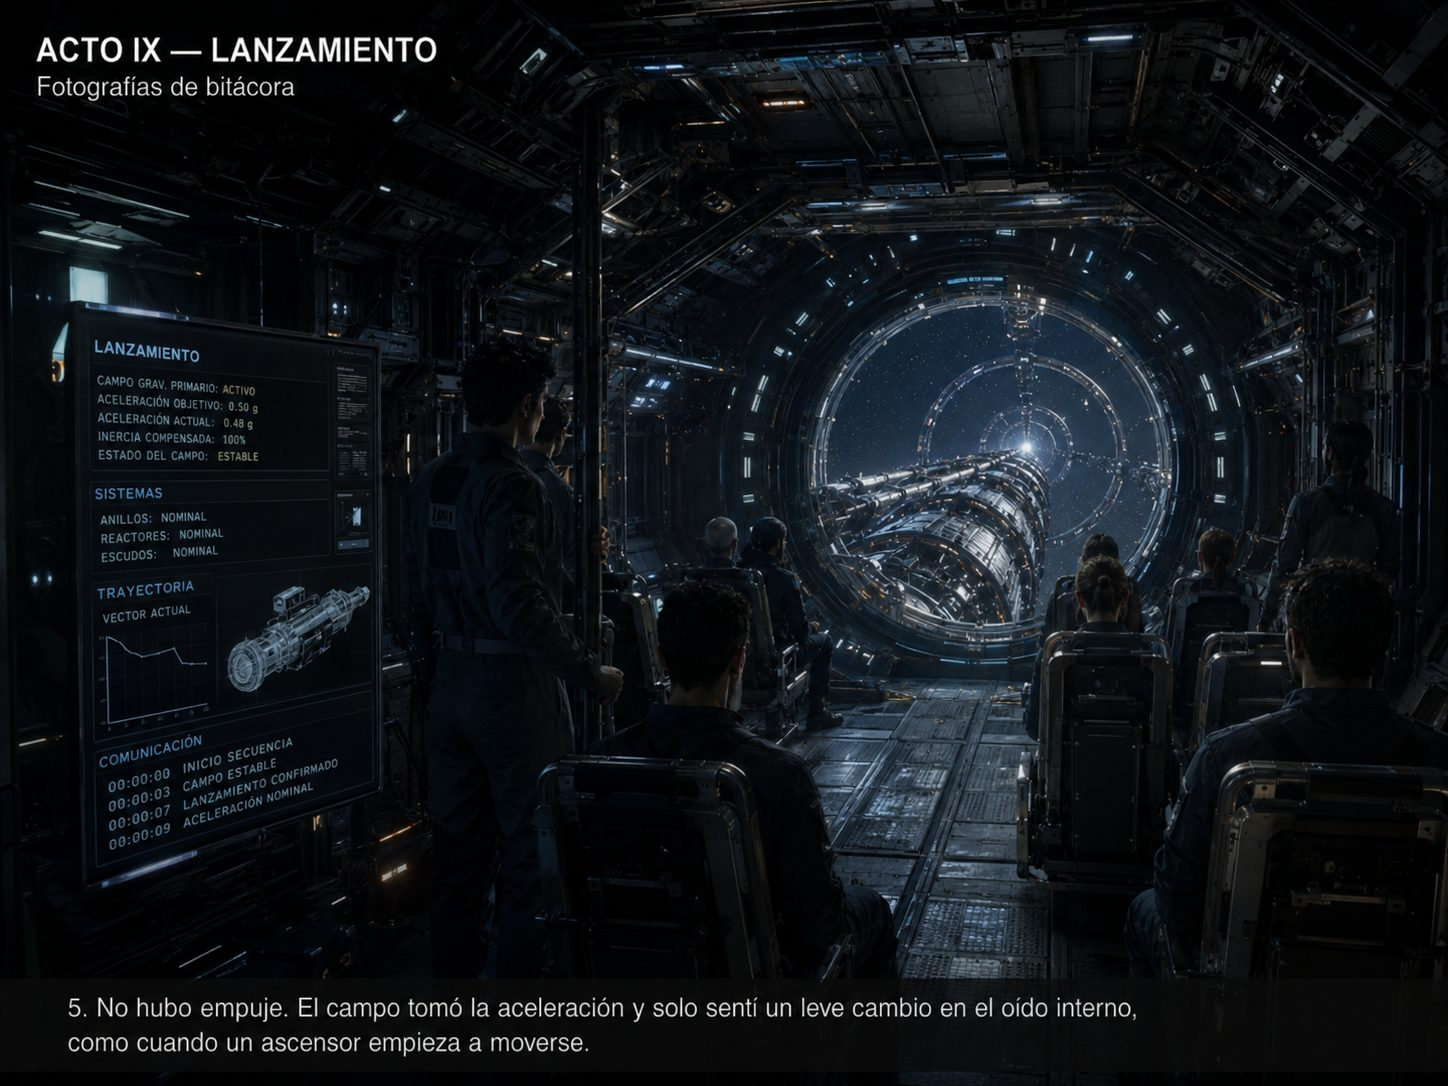
\includegraphics[width=0.9\textwidth]{09_5_lanzamientoenlanaveespacial.jpg}
\end{figure}

En la pantalla, los anillos quedaron atrás.

La Exterior se redujo. Primero una constelación artificial, luego un conjunto de puntos de luz, luego un punto entre muchos.

Júpiter y Saturno, visibles en la misma composición imposible, se convirtieron en dos faros antiguos que miraban en otra dirección.

\begin{figure}[h]
\centering
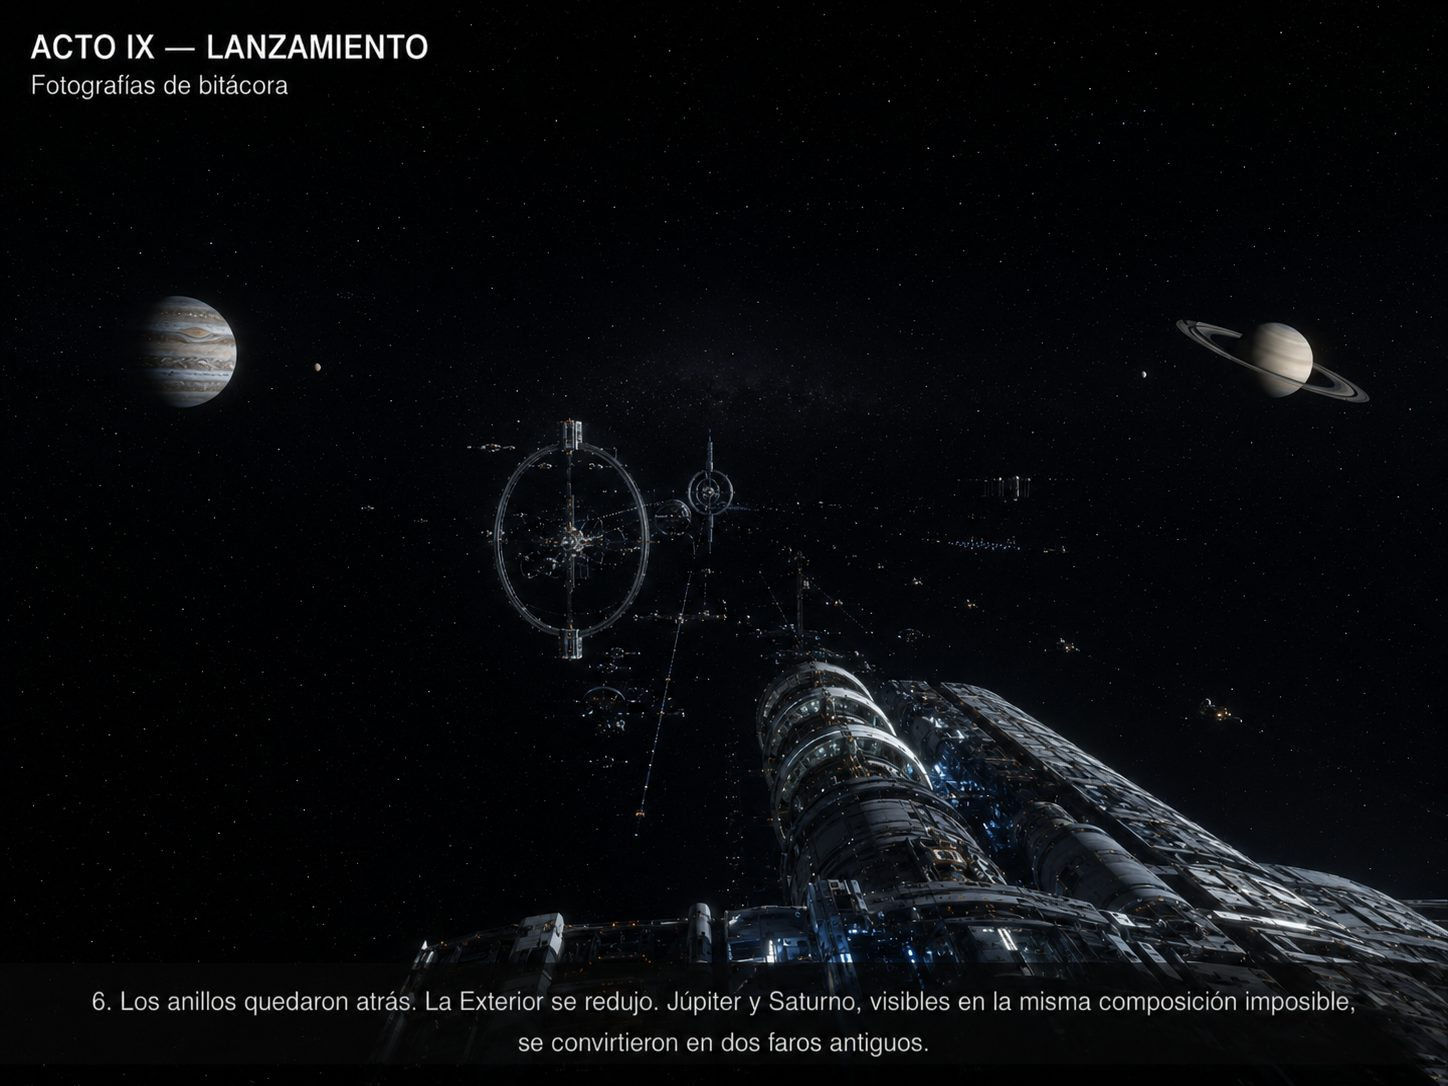
\includegraphics[width=0.9\textwidth]{09_6_lanzamientohacialosanilloslejanos.jpg}
\end{figure}

Luego el Sol dejó de ser el centro del cielo.

No de golpe. Poco a poco. Como todo lo importante.

\vspace{1.5em}
\begin{center}$\ast$\quad$\ast$\quad$\ast$\end{center}
\vspace{1.5em}

\chapter*{Acto X — Un año de noche}
\addcontentsline{toc}{chapter}{Acto X — Un año de noche}
\markboth{Acto X — Un año de noche}{Acto X — Un año de noche}

*\textit{Días 102–424. Atenea Larga. Espacio interestelar. 4,7c efectivos en burbuja warp.}*

El crucero interestelar no era emocionante.

Eso fue lo más difícil de aceptar.

La primera semana todos vivíamos pegados a las pantallas. Mirábamos el sistema solar encogerse, los planetas convertirse en puntos, el Sol perder dominancia sobre el campo visual. Había algo de ritual en ello: la despedida en cámara lenta que el espacio te permite hacer porque no hay nada que te apresure.

\begin{figure}[h]
\centering
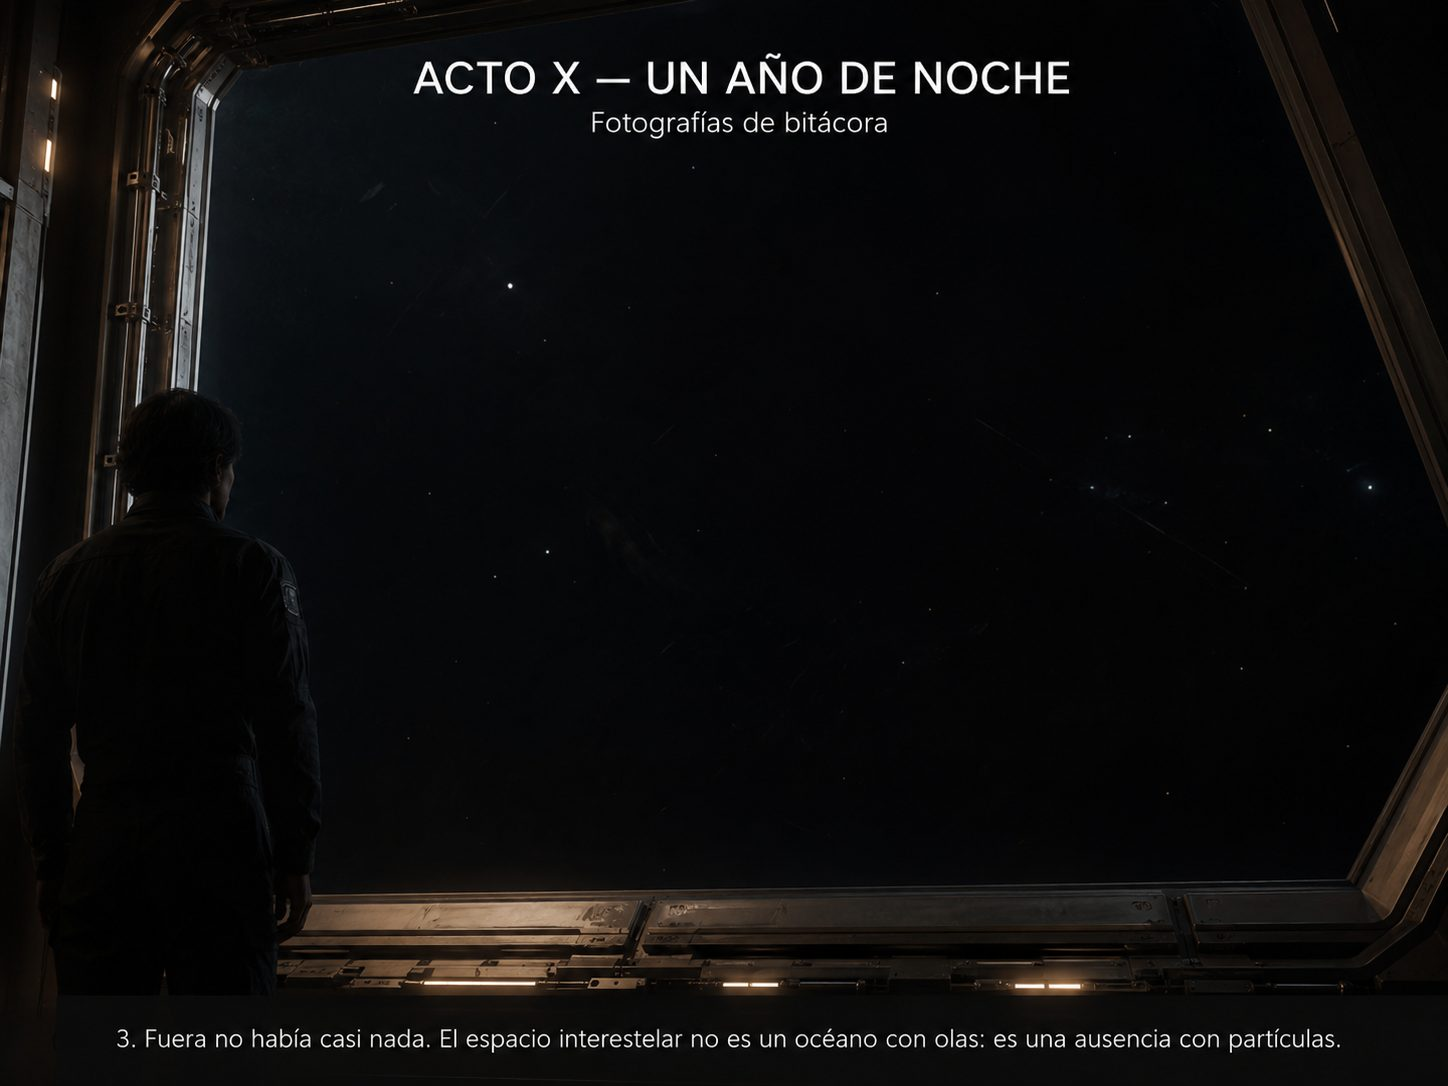
\includegraphics[width=0.9\textwidth]{10_1_actoxunaodenoche.jpg}
\end{figure}

La segunda semana empezaron las rutinas. No las rutinas de la emergencia o el trabajo urgente. Las rutinas de la vida normal: turnos de comida, horarios de ejercicio, reservas para los baños comunitarios, reuniones de sector por módulo habitacional.

La tercera semana hubo discusiones por espacios comunes. Una disputa sobre el volumen de la música en la zona de recreo del módulo cuatro. Una pelea menor por el uso de la lavandería industrial. Al mes, la Atenea Larga ya era una ciudad.

\begin{figure}[h]
\centering
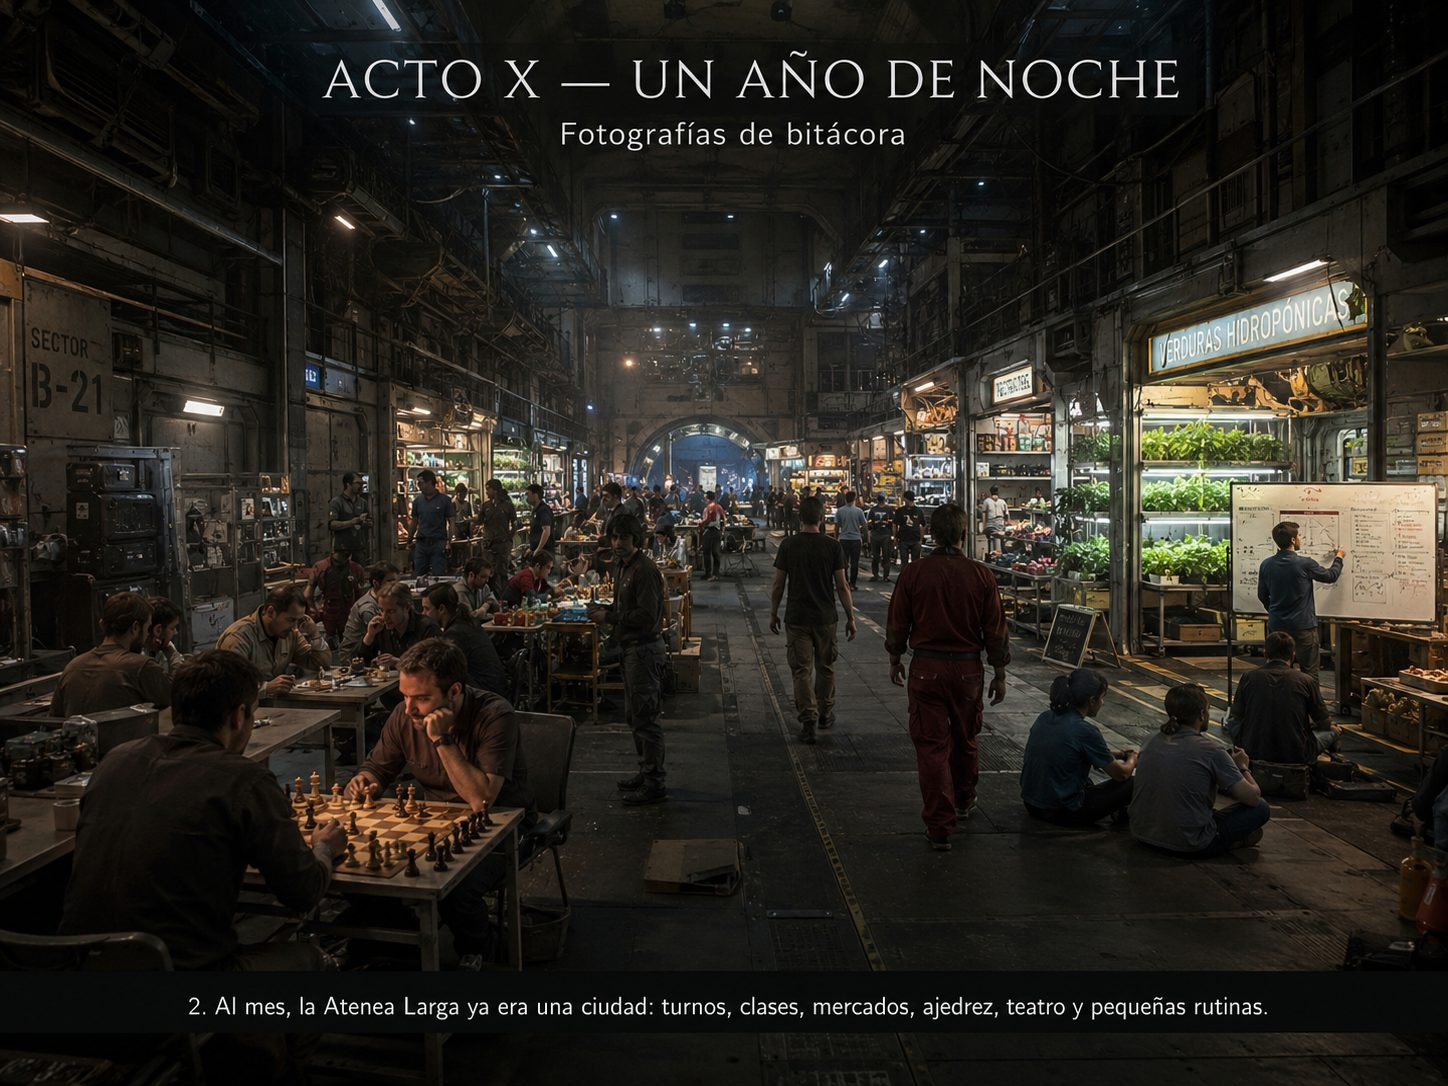
\includegraphics[width=0.9\textwidth]{10_2_mercadointerestelarenlaatenealarga.jpg}
\end{figure}

Tenía turnos de trabajo, clases para los doscientos niños a bordo, mercados internos donde se intercambiaban servicios y objetos fabricados, teatro amateur los fines de semana de tiempo estándar, duelos de ajedrez con tablero físico porque alguien había insistido en traerlo, entrenamientos físicos obligatorios para mantener la musculatura en 0,4g, cultivos hidropónicos en el módulo seis que suministraban el veinte por ciento de los vegetales, enfermedades leves que pasaban de sección en sección con la inevitable velocidad de los espacios cerrados, romances que nacían rápido y terminaban más rápido aún en la presión de vivir a tres metros de todo el mundo.

Fuera no había casi nada.

El espacio interestelar no es un océano con olas. Es una ausencia con partículas. Entre los sistemas solares, la densidad de materia baja hasta niveles que hacen del vacío terrestre algo casi denso por comparación. No hay viento solar aquí. No hay magnetosfera de ningún planeta cercano. Hay radiación cósmica, neutrinos, polvo interestelar a velocidades que en campo libre serían inofensivas y dentro de la burbuja a 4,7c efectivos representaban otra clase de problema.

\begin{figure}[h]
\centering
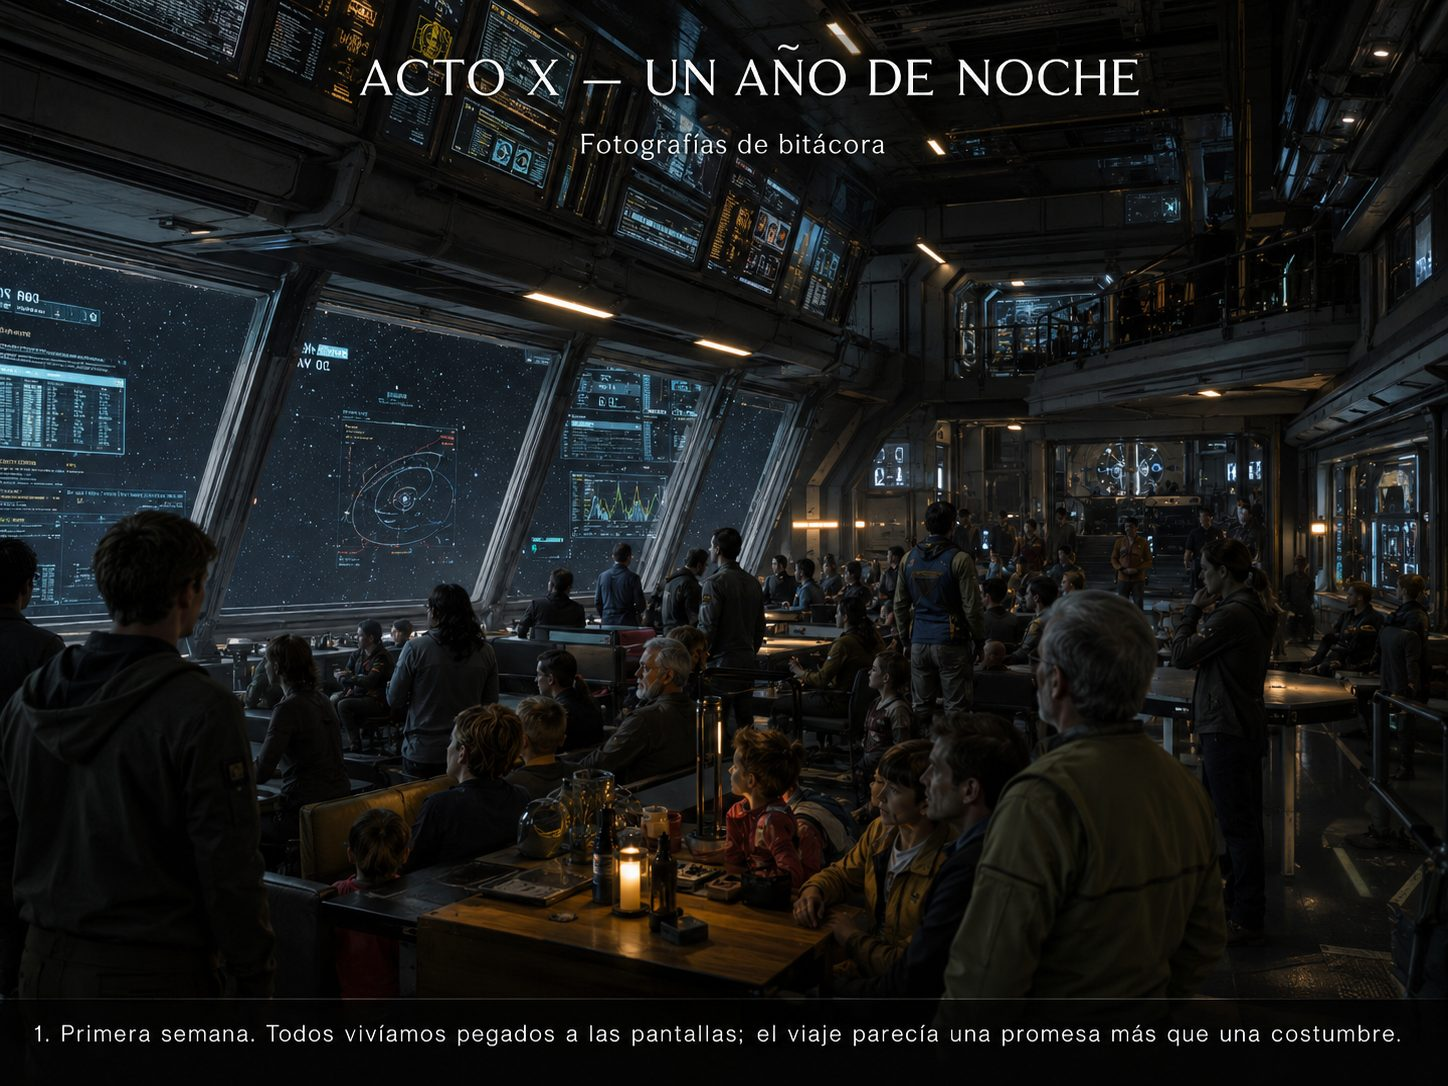
\includegraphics[width=0.9\textwidth]{10_3_vistaespacialenlanave.jpg}
\end{figure}

El escudo frontal recibía impactos microscópicos cada día. Los sistemas los registraban con la calma de lo que han visto ya muchas veces: masa estimada, energía de impacto, dispersión en el material del escudo, protocolo de reparación o simplemente registro si el impacto estaba dentro de la tolerancia. Lo llamaban «lluvia técnica». A 4,7c efectivos dentro de burbuja, incluso lo pequeño merecía respeto.

\begin{figure}[h]
\centering
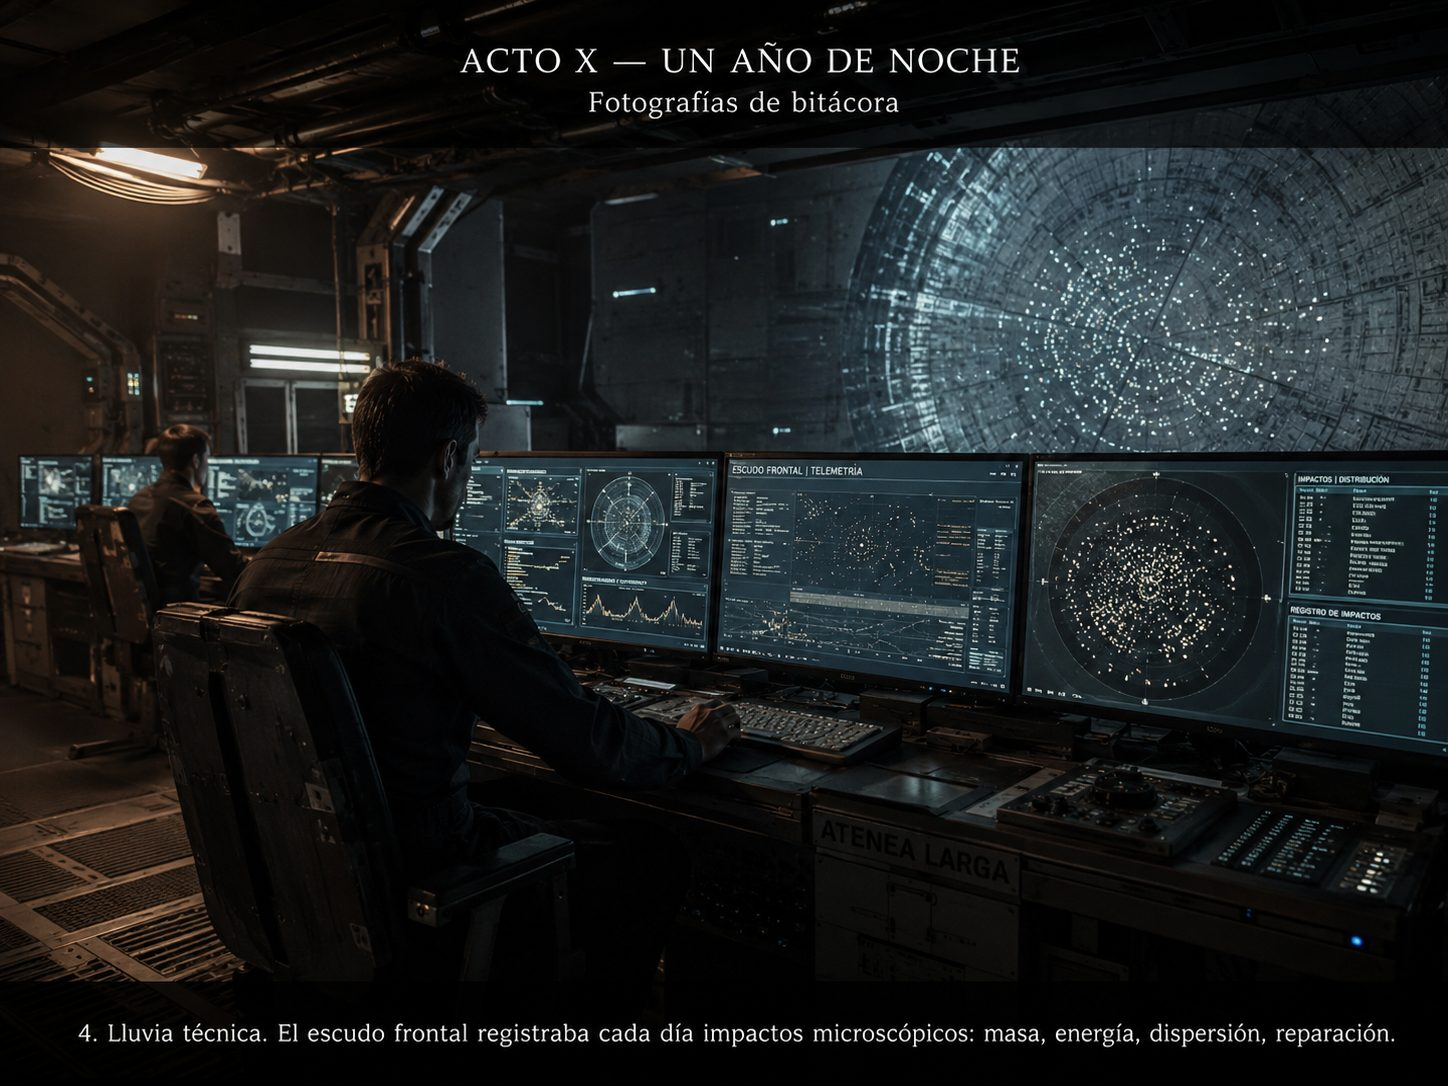
\includegraphics[width=0.9\textwidth]{10_4_controloperativodelescudofrontal.jpg}
\end{figure}

Cada mes hacíamos una ceremonia mínima: mirar hacia atrás.

\begin{figure}[h]
\centering
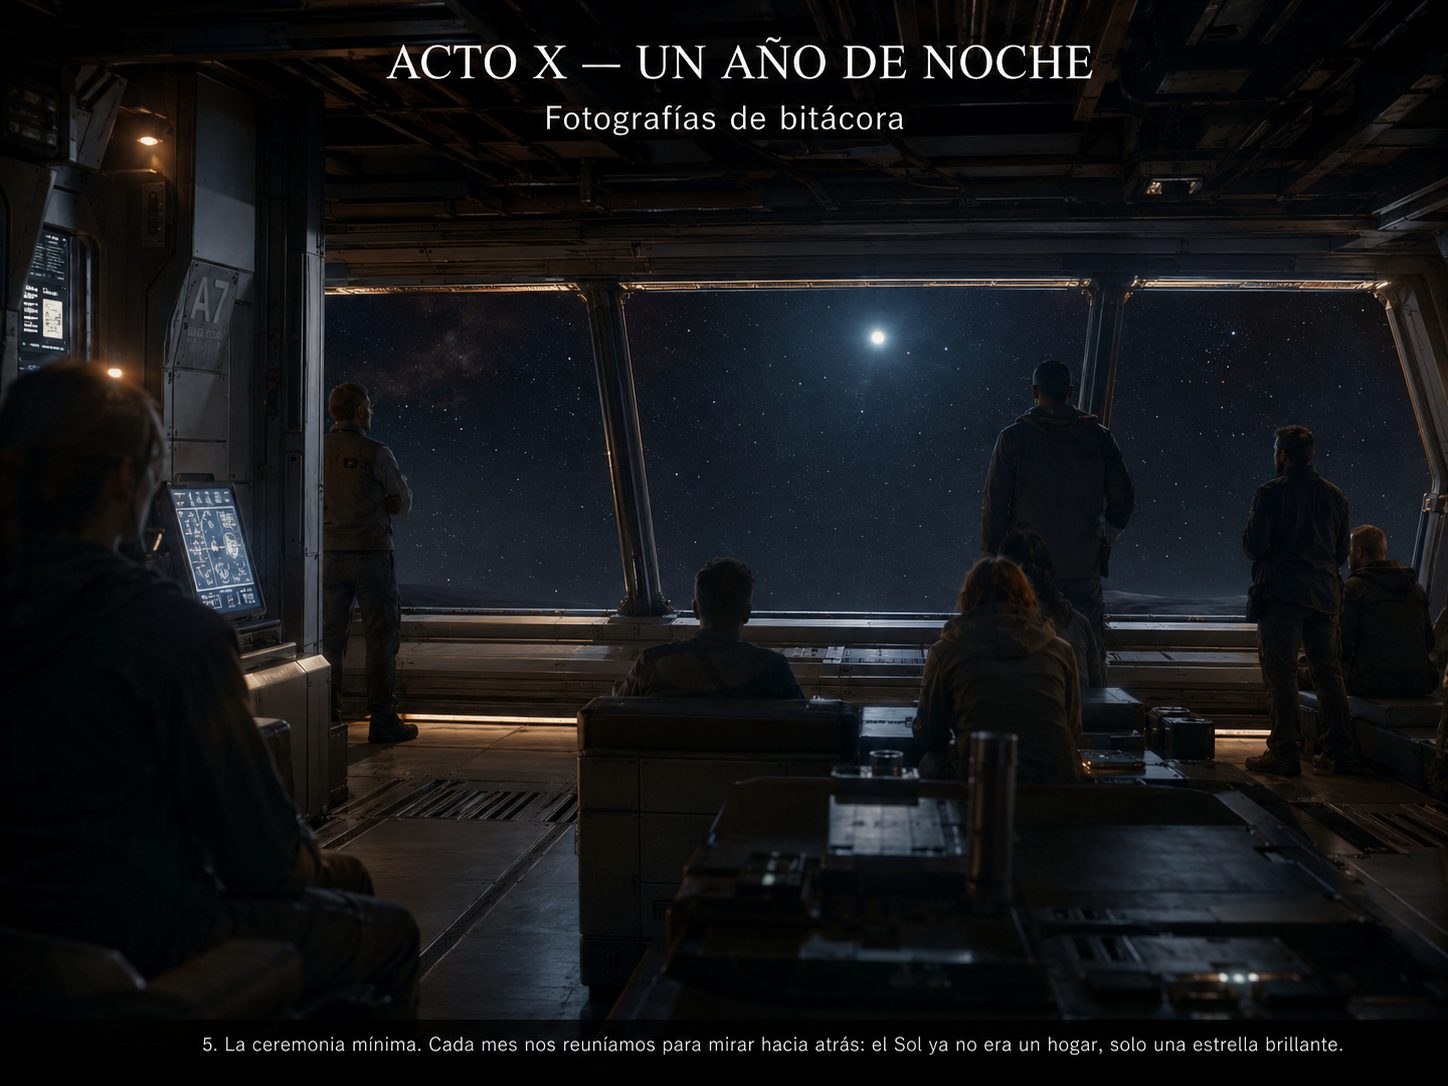
\includegraphics[width=0.9\textwidth]{10_5_loungeespacialenlapenumbra.jpg}
\end{figure}

En la sala de observación de popa —la única con vista hacia el sistema solar de origen— se congregaba la mayor parte de la población activa de la nave. No todos. Nunca todos. Pero bastantes para que el silencio tuviera peso.

El Sol se convirtió en una estrella brillante en el primer mes. Todavía la más brillante. Todavía distinguible con certeza en el campo visual.

En el segundo mes, seguía siendo la más brillante, pero ya no era obvia. Había que saber dónde mirar.

En el cuarto mes, era una entre las más brillantes. No la única candidata.

Al sexto mes, algunos dejaron de asistir a la ceremonia mensual. No por indiferencia, creo. Por algo más complicado: porque mirar ya no era ver algo claro, y la ambigüedad era más difícil de sostener que la ausencia.

Yo no dejé de asistir.

Hay algo que necesita ser testigo, aunque ya no haya nada claro que testimoniar.

En mi diario escribí, en algún momento del quinto mes, sin fecha precisa porque los días ya habían perdido el anclaje al planeta:

> La Tierra no desaparece de golpe. Se convierte lentamente en una idea.

\begin{figure}[h]
\centering
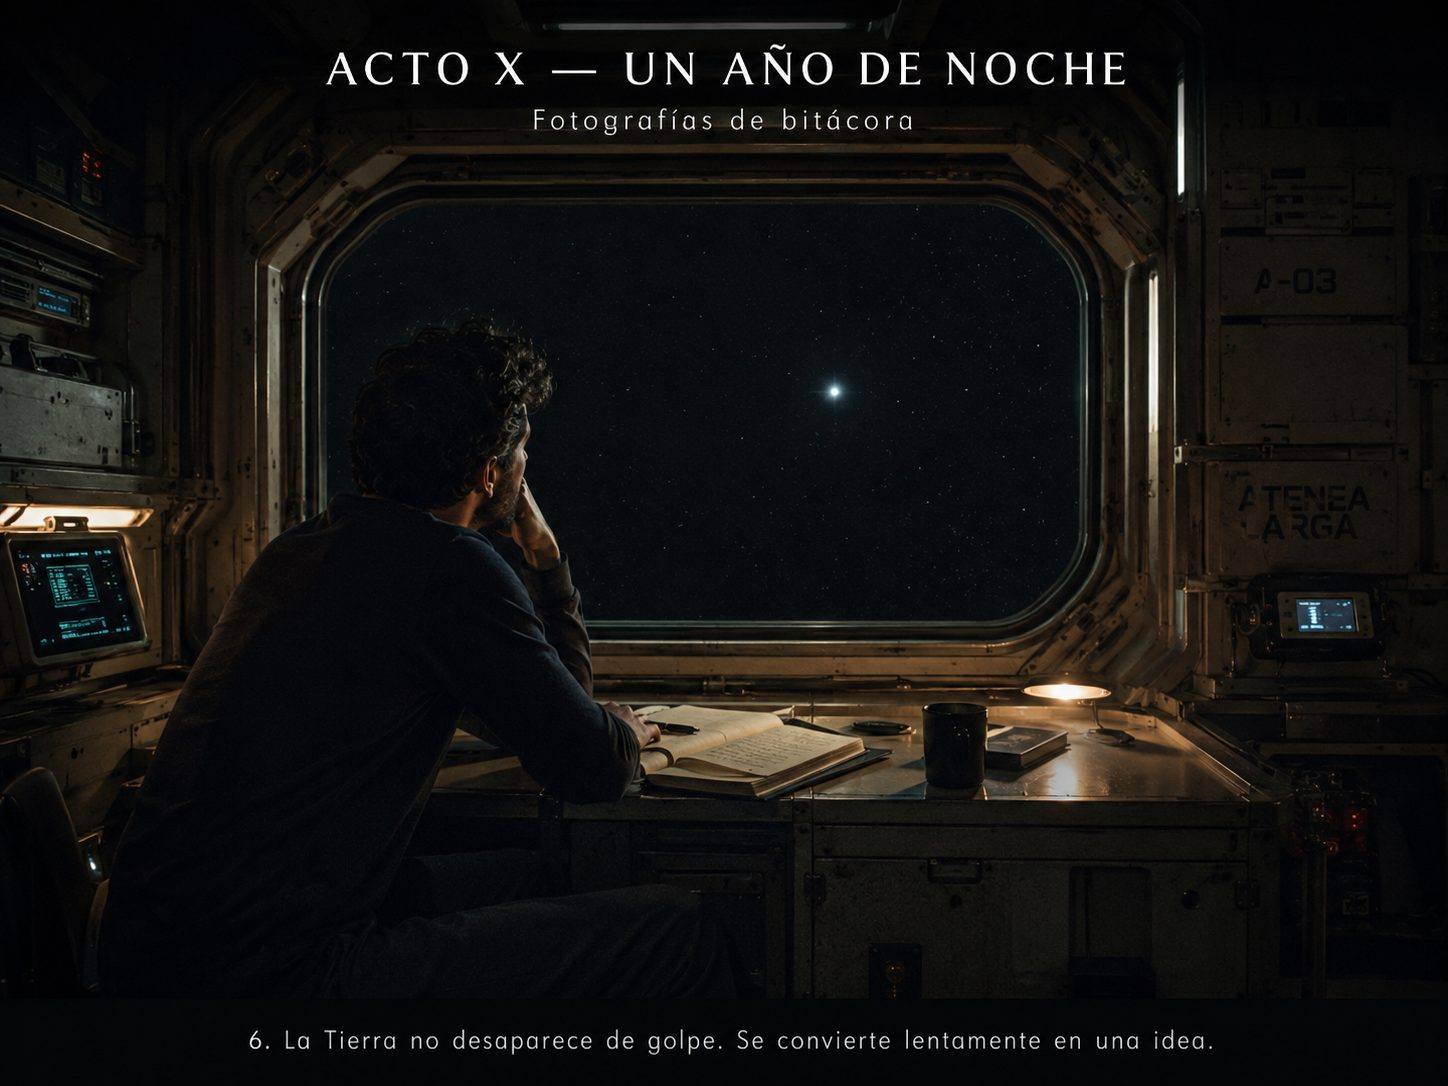
\includegraphics[width=0.9\textwidth]{10_6_reflexionesenlanaveatenea.jpg}
\end{figure}

Y luego, más abajo, como si hubiera querido completar el pensamiento días después:

> Pero las ideas no son menos reales. A veces son más.

\vspace{1.5em}
\begin{center}$\ast$\quad$\ast$\quad$\ast$\end{center}
\vspace{1.5em}

\chapter*{Acto XI — La sombra de Centauri}
\addcontentsline{toc}{chapter}{Acto XI — La sombra de Centauri}
\markboth{Acto XI — La sombra de Centauri}{Acto XI — La sombra de Centauri}

*\textit{Días 425–466. Atenea Larga. Desaceleración de campo. Sistema de Alpha Centauri.}*

El primer signo de llegada no fue Alpha Centauri.

Fue el cambio de turnos.

\begin{figure}[h]
\centering
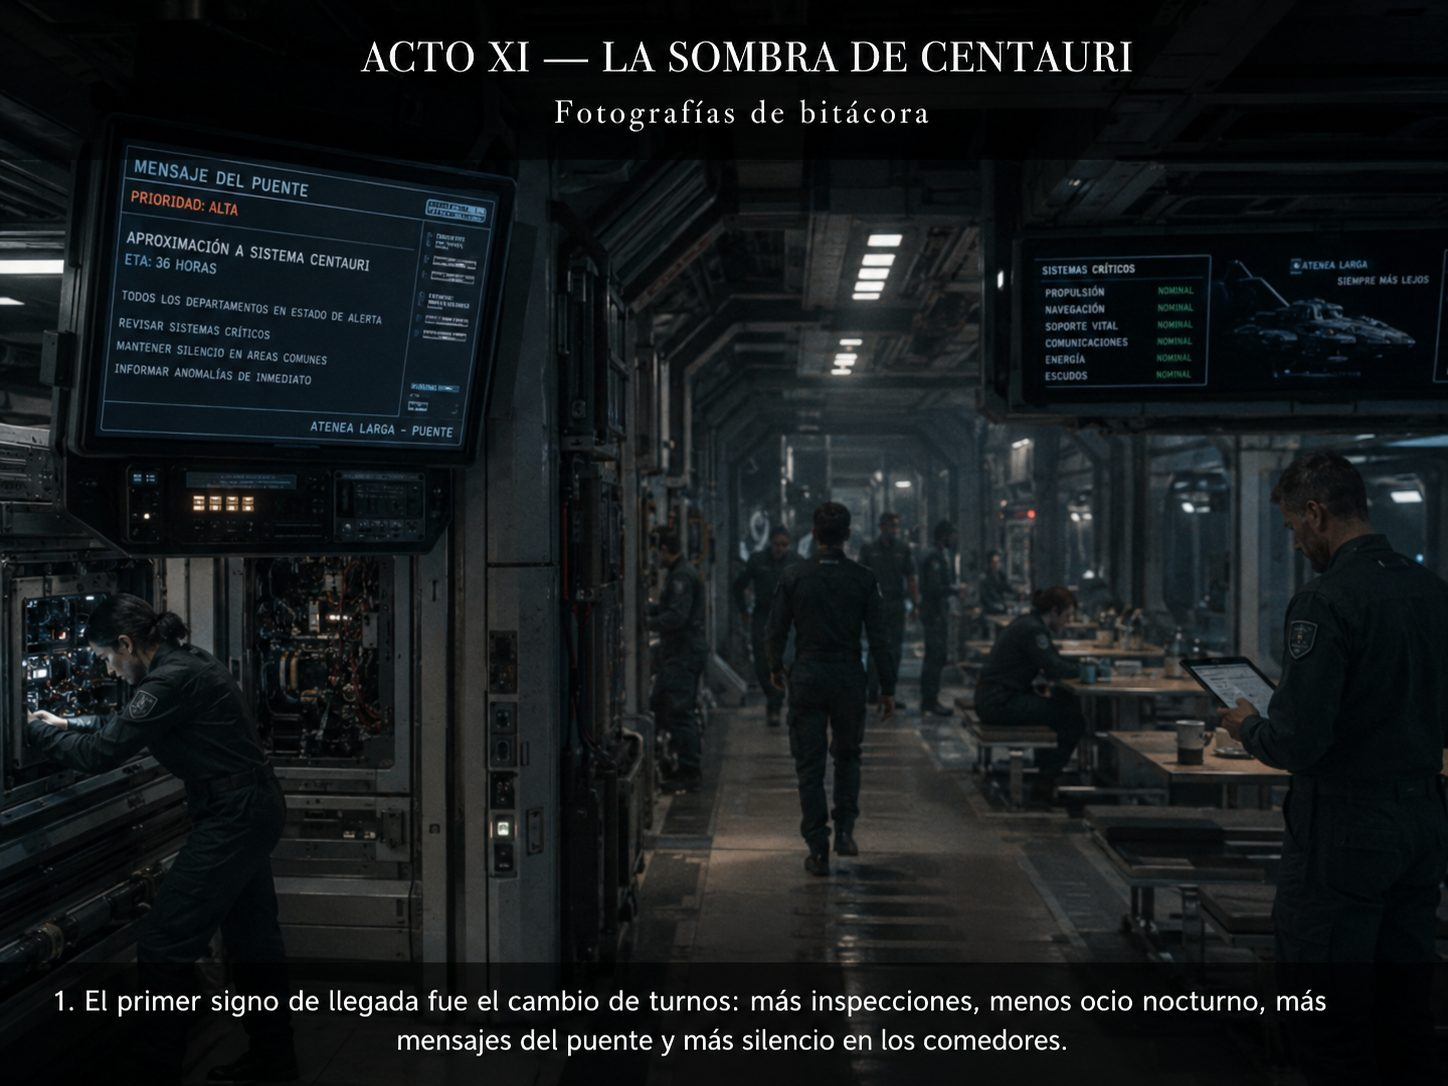
\includegraphics[width=0.9\textwidth]{11_1_interiordenaveenalerta.jpg}
\end{figure}

La nave entera empezó a comportarse de otra manera unas semanas antes de que los sensores confirmaran que estábamos en rango de aproximación real. Más inspecciones de rutina que se volvían no rutinarias. Menos ocio nocturno en los espacios comunes. Más mensajes del puente para jefes de sección. Más silencio en los comedores, no el silencio incómodo de los primeros meses del crucero, sino el silencio de la concentración antes de algo que importa.

La gente lo sabía aunque no lo supiera. El organismo colectivo de la nave lo procesaba antes que la mente individual.

La desaceleración de campo comenzó cuarenta y un días antes de la llegada oficial.

\begin{figure}[h]
\centering
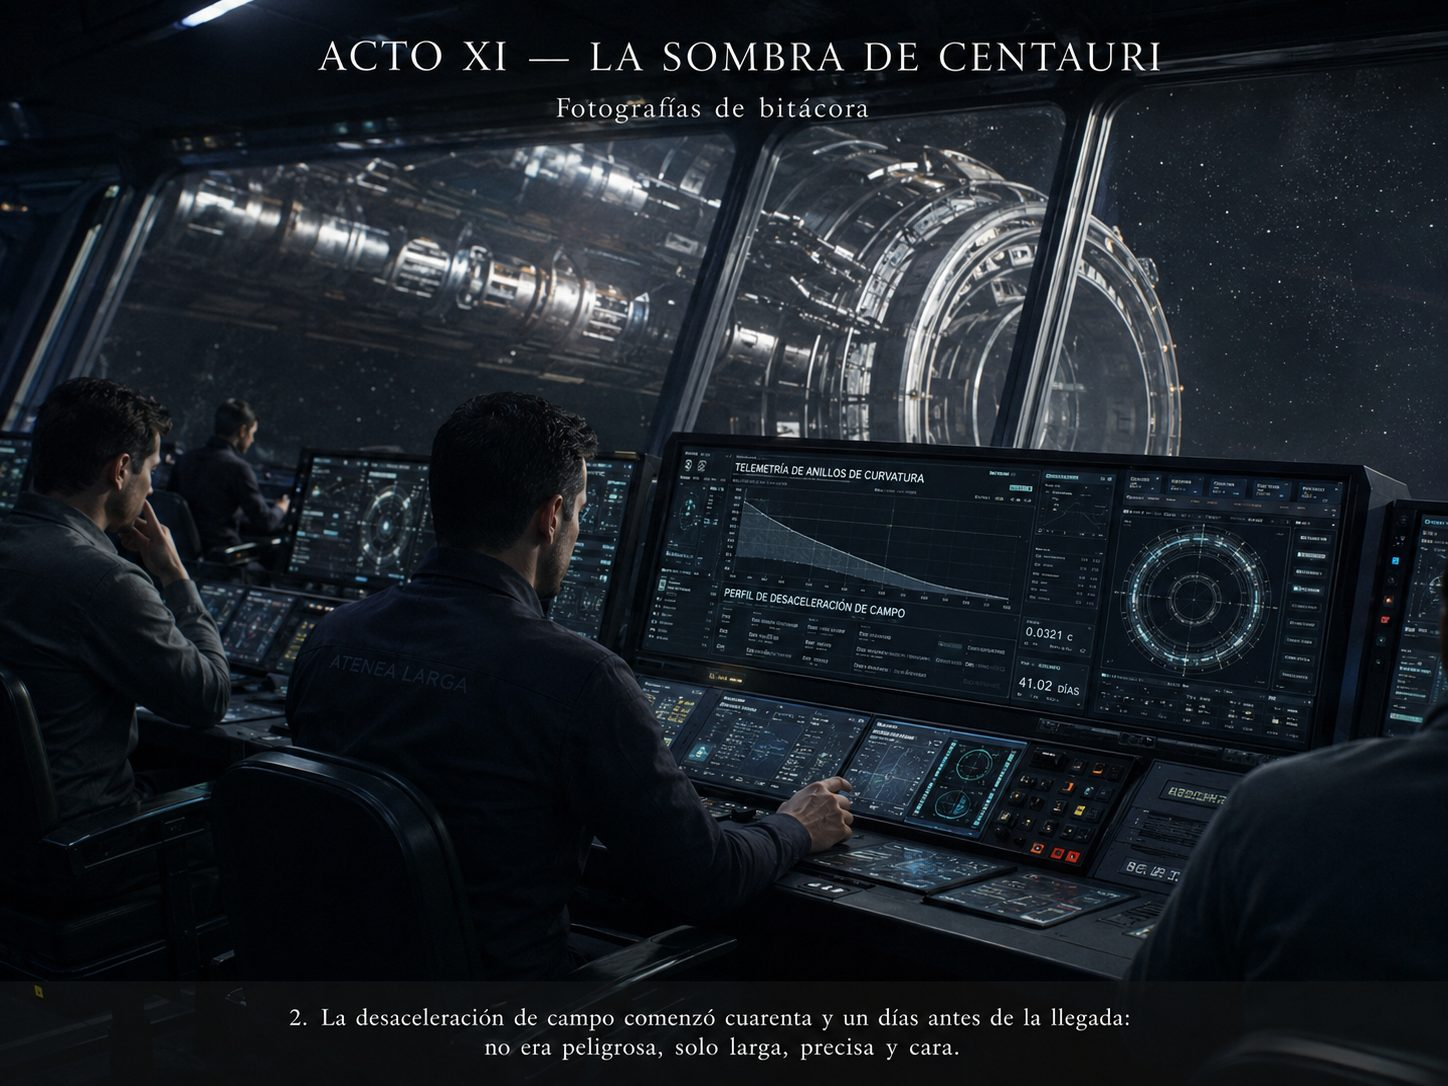
\includegraphics[width=0.9\textwidth]{11_2_puentedecontrolenlaoscuridadespacial.jpg}
\end{figure}

Sin catapulta de destino en el sistema de Alpha Centauri, la Atenea Larga debía hacer casi todo el trabajo con sus propios anillos. No era peligroso, decía el comunicado oficial de la capitana. Solo largo, preciso y energéticamente caro. Los reactores de fusión trabajaron al máximo de su régimen durante todo ese período. Los bancos superconductores, que habían estado en modo de reserva durante la mayor parte del crucero, se vaciaron y llenaron en ciclos cada vez más frecuentes.

Un ingeniero de propulsión lo resumió en los términos más honestos que encontré durante todo el viaje:

—Salir fue como ser lanzados por una montaña. Llegar es bajar esa montaña con una cuerda.

\begin{figure}[h]
\centering
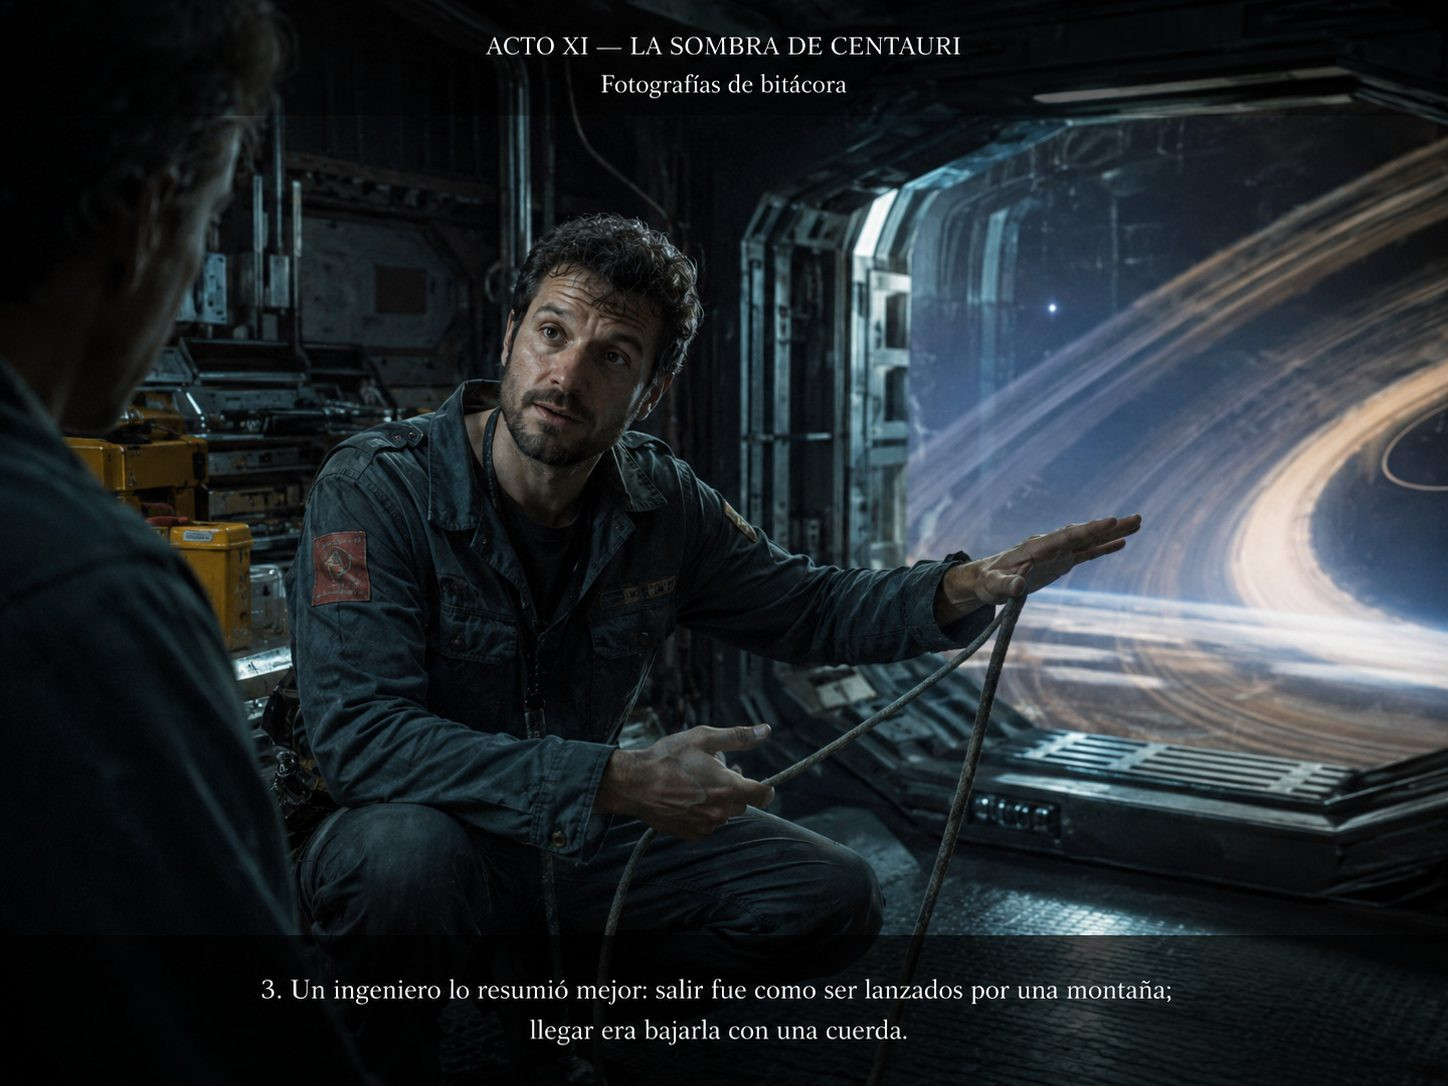
\includegraphics[width=0.9\textwidth]{11_3_ingenieroeneltallerespacial.jpg}
\end{figure}

La metáfora no era perfecta —no hay montaña, no hay cuerda, solo geometría de espacio-tiempo negociada con campos superconductores— pero era verdad en lo que importaba. Salir había sido externo, colectivo, asistido. Llegar era interno, propio, sin red.

Alpha Centauri A apareció como un sol verdadero, no como un punto.

Ese fue el momento. No el anuncio oficial de aproximación. No los datos en los sensores. El momento fue cuando levanté la vista de la pantalla y pensé: eso no es una estrella. Eso es un sol. Amarillo-blanco, sin el centelleo que da la atmósfera terrestre, perfectamente quieto en el campo visual. Un sol que no era el mío pero que calentaba con la misma clase de física.

Después vimos Alpha Centauri B, más anaranjada, en su propia posición del sistema binario. Y Próxima era apenas una chispa roja en los sensores exteriores, demasiado lejos para el ojo humano no asistido.

\begin{figure}[h]
\centering
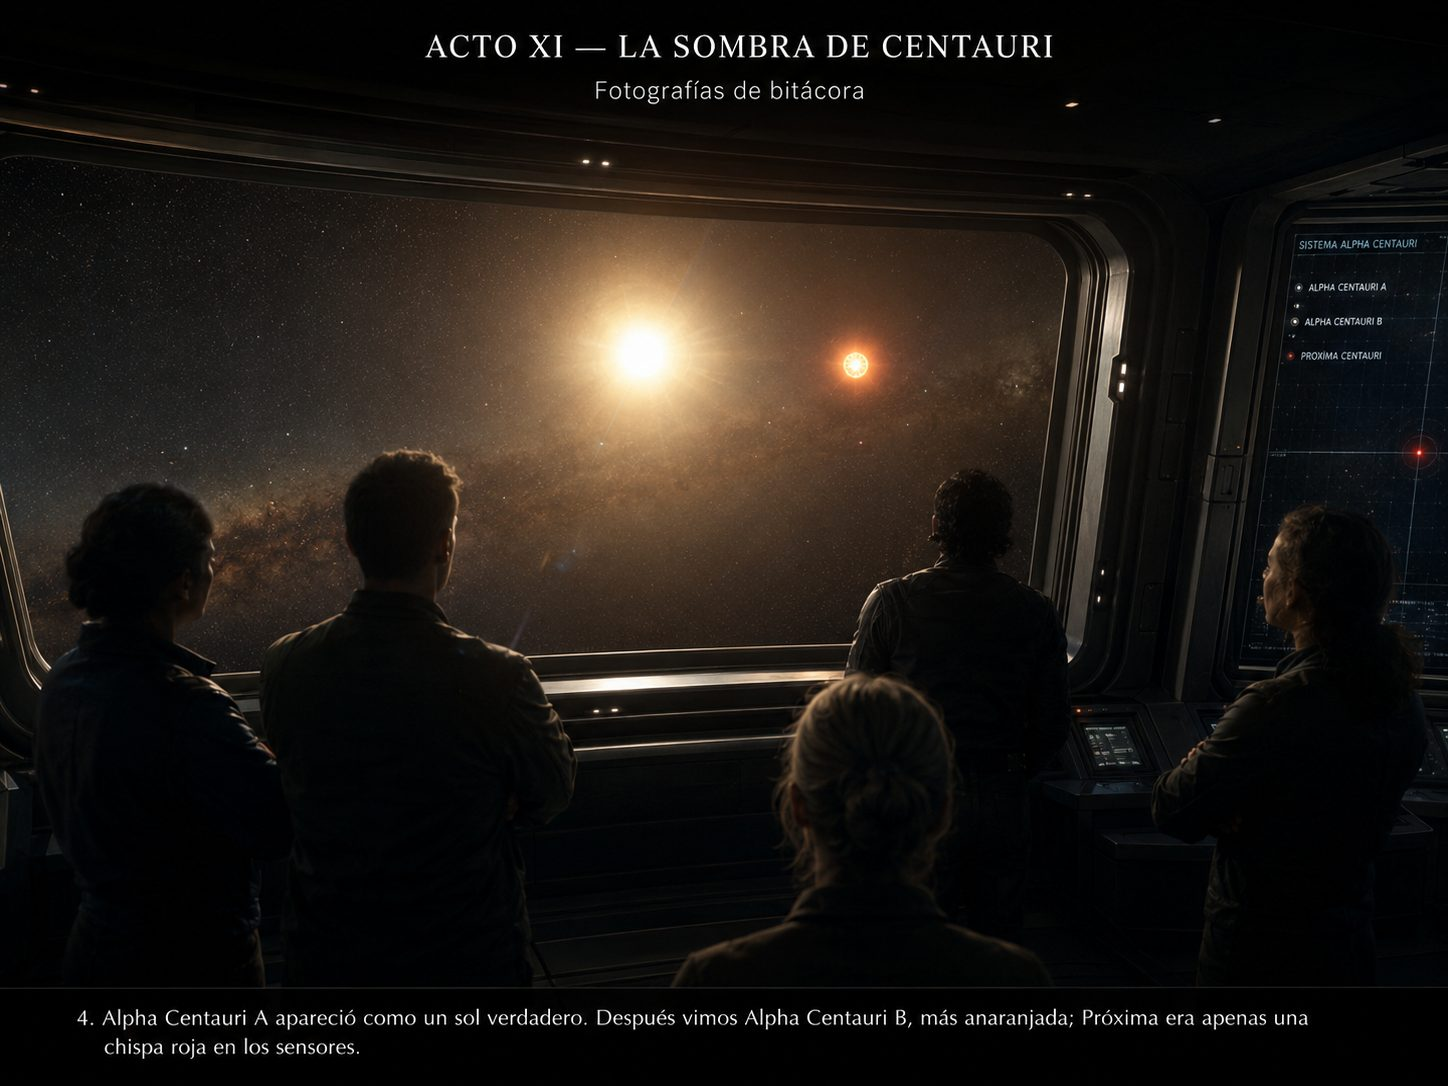
\includegraphics[width=0.9\textwidth]{11_4_observatorioenlaestacinespacial.jpg}
\end{figure}

La colonia no estaba en un planeta. Todavía no.

*\textit{Nueva Concordia}\textit{ era un enjambre en construcción alrededor de un mundo candidato: estaciones pequeñas, hábitats modulares de montaje reciente, depósitos de recursos, espejos de concentración solar para energía, laboratorios atmosféricos flotantes que analizaban el exoplaneta desde arriba, módulos de descenso listos para las expediciones de superficie. El planeta, llamado provisionalmente }\textit{Concordia-b}*, tenía nubes visibles en el espectro óptico, océanos oscuros —más oscuros que los terrestres, probablemente por la composición de la superficie bajo el agua—, y continentes aún no cartografiados con nombres definitivos.

\begin{figure}[h]
\centering
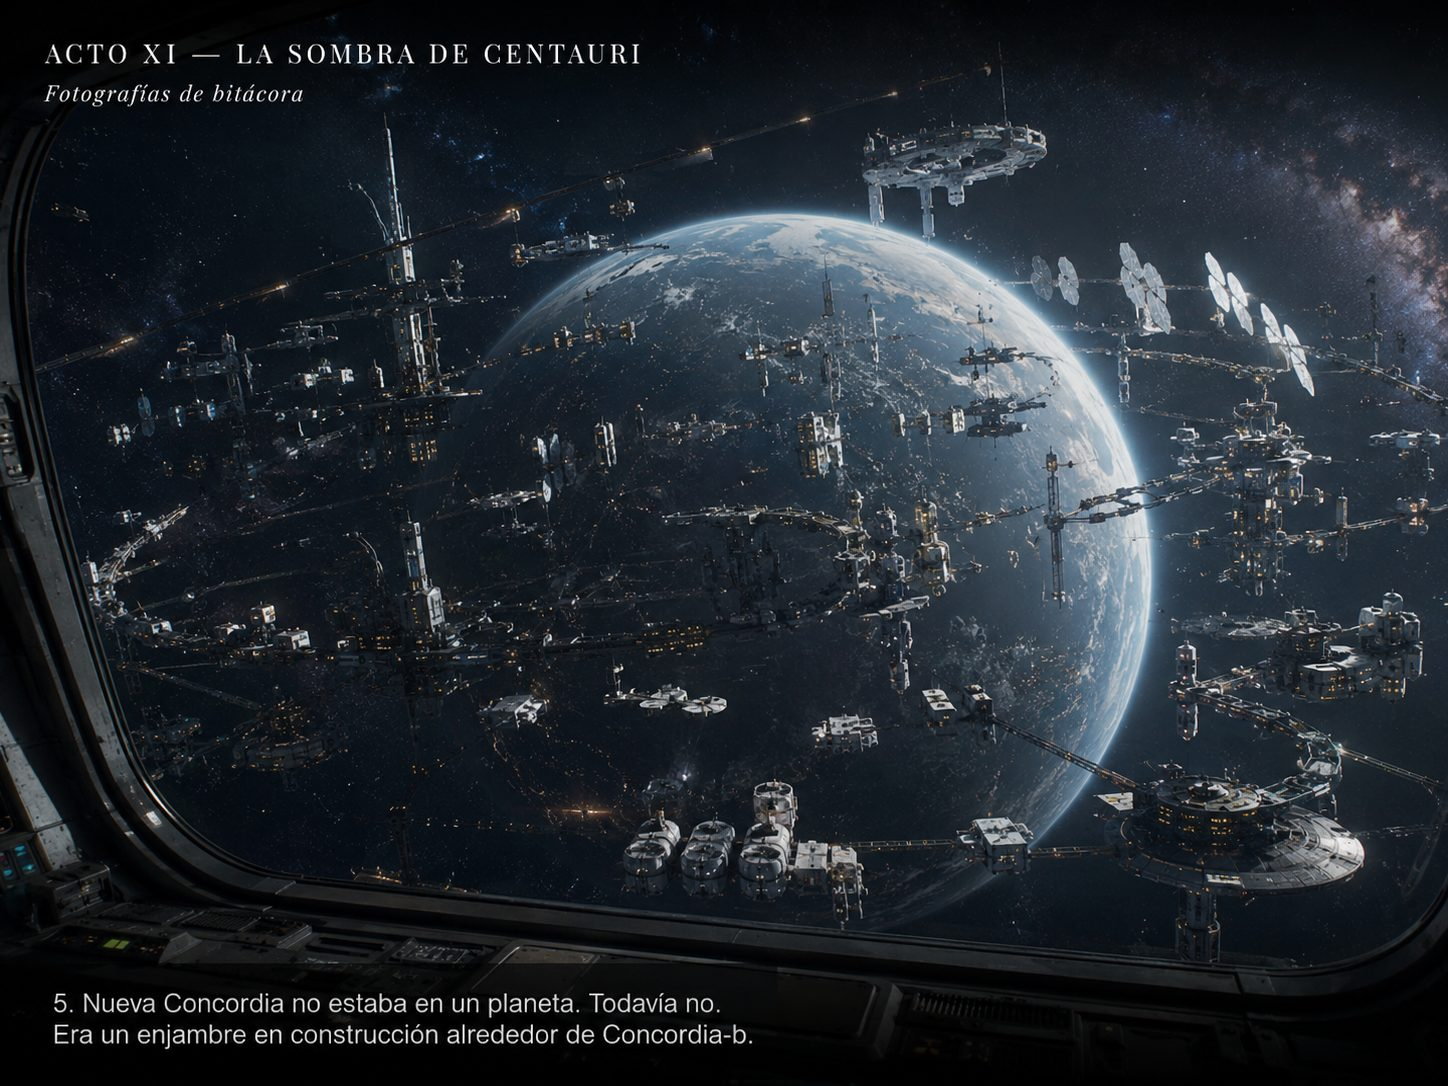
\includegraphics[width=0.9\textwidth]{11_5_estacinenconstruccinalrededordeconcordiab.jpg}
\end{figure}

Había estados de ánimo distintos en la nave durante esos últimos días.

Algunos lloraban de alegría sin poder explicarlo bien. Otros estaban callados con una quietud que no era tristeza sino algo más difícil de nombrar: la conclusión de algo que había definido un año entero de su vida. Algunos estaban ya calculando el regreso, el largo regreso sin catapulta a 1,3c, más de tres años. Otros parecían haberlo decidido: esta era ahora su estrella.

Yo miraba a Concordia-b desde los sensores ópticos.

No era otra Tierra.

Eso nos lo habían repetido mil veces antes del viaje, durante el viaje, en cada comunicado oficial que establecía expectativas. No era otra Tierra. No lo sería en décadas, probablemente no en siglos.

No era otra Tierra.

Pero tenía horizonte.

\begin{figure}[h]
\centering
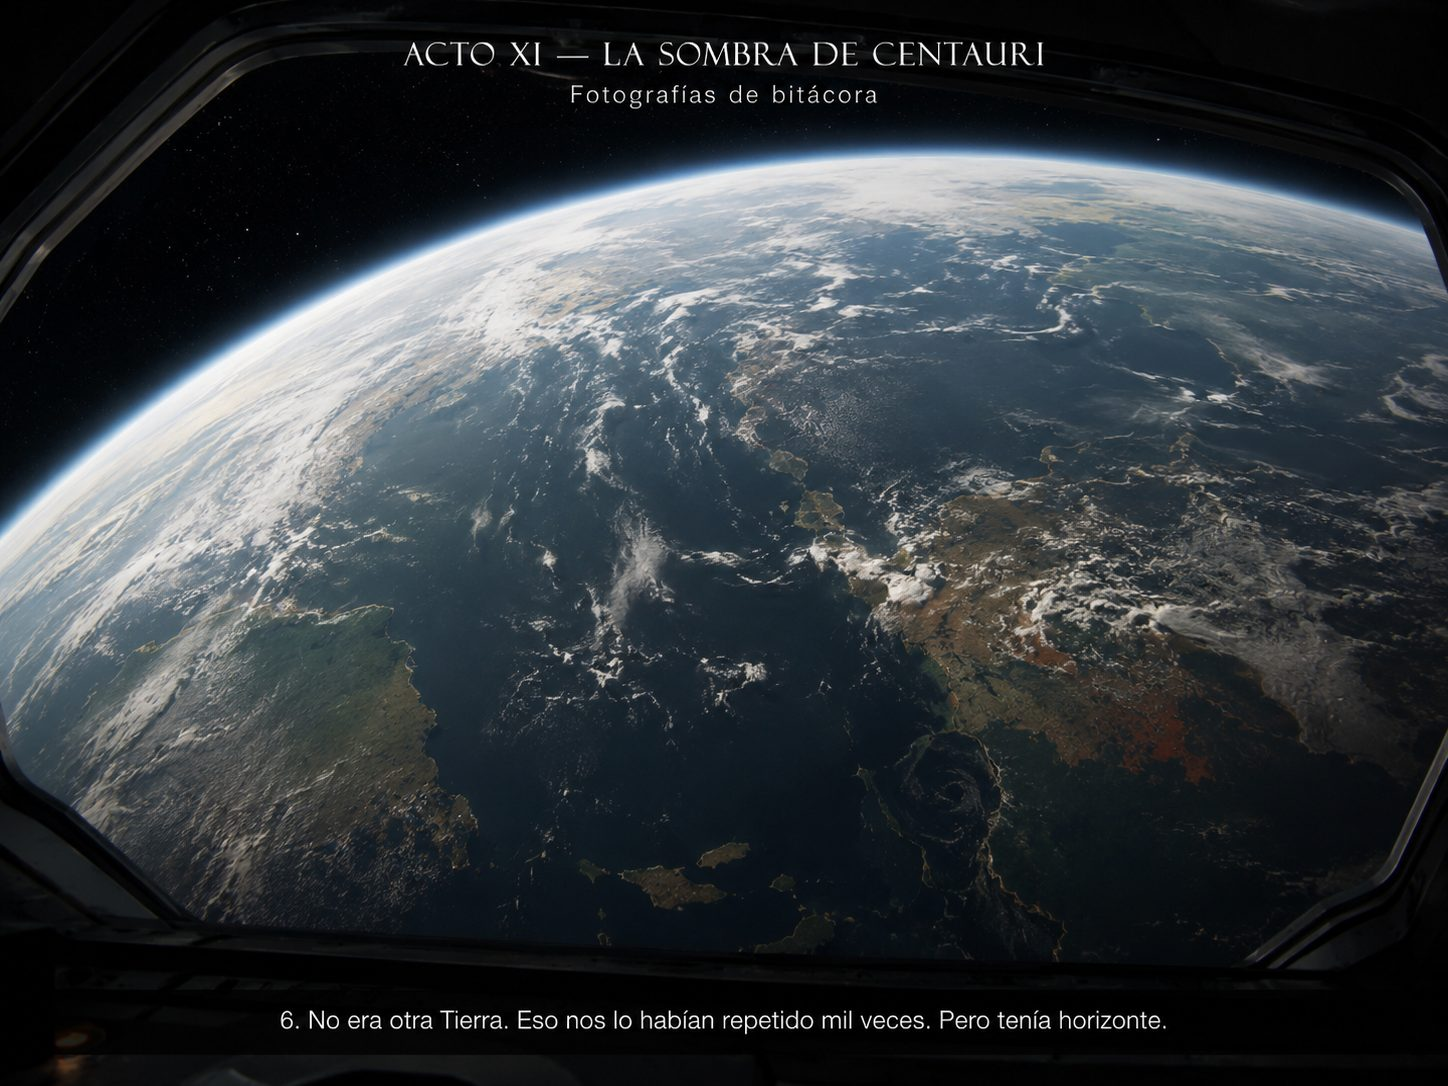
\includegraphics[width=0.9\textwidth]{11_6_vistaorbitaldesdelanave.jpg}
\end{figure}

Y eso, a estas distancias, era casi suficiente.

\vspace{1.5em}
\begin{center}$\ast$\quad$\ast$\quad$\ast$\end{center}
\vspace{1.5em}

\chapter*{Epílogo — Nueva Concordia}
\addcontentsline{toc}{chapter}{Epílogo — Nueva Concordia}
\markboth{Epílogo — Nueva Concordia}{Epílogo — Nueva Concordia}

*\textit{Día 467. Lanzadera de descenso. Concordia-b. Sistema de Alpha Centauri A.}*

El último tramo lo hice en una lanzadera pequeña.

Después de un año en la Atenea Larga, la nave de descenso parecía ridícula. Frágil. Cercana. Humana a una escala que la nave interestelar ya había dejado de ser. Cabía en ella en catorce personas y el equipaje de mano de catorce personas, y el asiento crujió cuando me senté. El asiento crujió. En una nave que iba a cruzar la atmósfera de un mundo a cuatro años luz de la Tierra, el asiento crujía como los de los autobuses viejos.

Me pareció una señal esperanzadora.

Pasamos junto a los primeros astilleros centaurianos durante la bajada. Eran pequeños comparados con Ceres o La Exterior, casi humildes: estructuras de montaje reciente con el brillo del metal no envejecido, módulos de hábitat en diferentes estadios de construcción, sistemas de drones que trabajaban en la oscuridad entre los andamios. Pero tenían algo que ninguna estación del sistema solar poseía.

\begin{figure}[h]
\centering
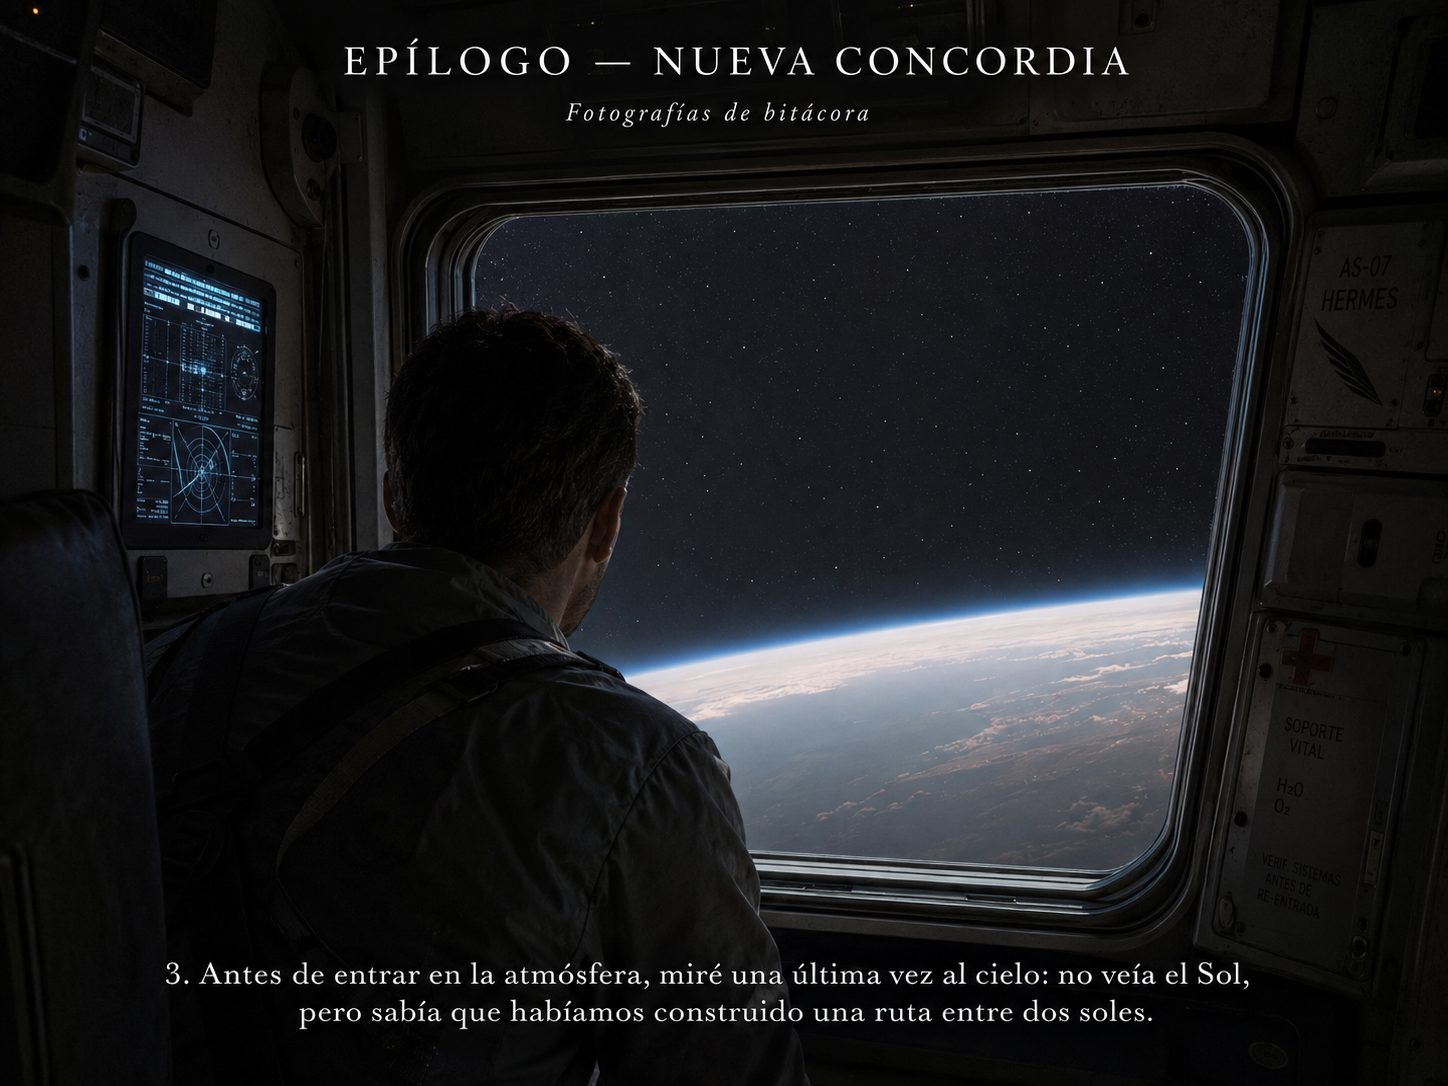
\includegraphics[width=0.9\textwidth]{12_1_ltimamiradaantesdereentrada.jpg}
\end{figure}

Estaban solos.

No había red detrás. No había siglos de industria acumulada alrededor. No había rescate rápido, ni suministro garantizado, ni alternativa preparada para cuando algo fallara. Todo lo que Nueva Concordia era, lo había traído a bordo de las últimas seis misiones o lo estaba fabricando con sus propias manos y sus propias máquinas, a cuatro años de la siguiente fuente de ayuda.

\begin{figure}[h]
\centering
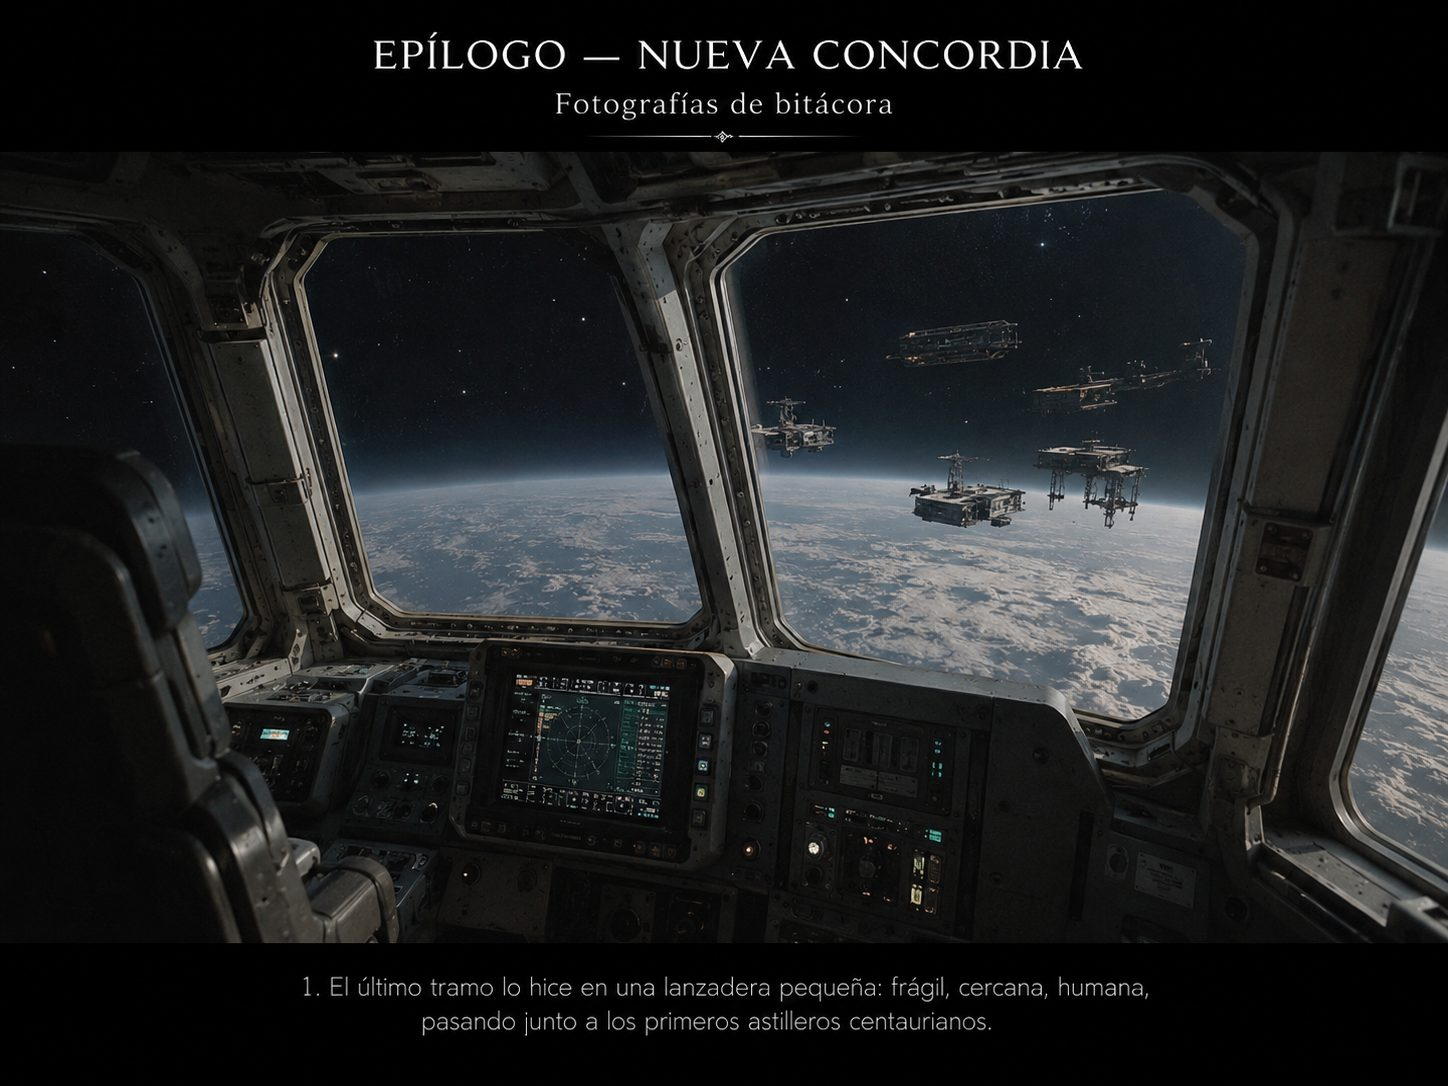
\includegraphics[width=0.9\textwidth]{12_2_epilogoenelespacioprofundollegandoanuevaconcordia.jpg}
\end{figure}

Eso cambiaba el tamaño de todo lo que habían construido.

Antes de entrar en la atmósfera alta de Concordia-b, miré una última vez hacia el cielo.

No podía ver el Sol. No a simple vista, con el campo visual lleno del planeta candidato y la luz de Alpha Centauri A filtrándose por la ventanilla lateral. Pero sabía que estaba allí: una estrella entre las estrellas, perdida en el campo de la constelación que los futuros habitantes de este mundo llamarían con otro nombre. Y girando a su alrededor, la Tierra, y el Puerto Cislunar, y Fobos con sus correctores de milímetros de paciencia, y Ceres fabricando piezas, y Calisto con sus bares donde pilotos que no bajan a planetas hablan de lo que han visto, y Titán naranja y tóxico y productivo, y La Exterior con su pregunta hecha de anillos.

Una ruta tendida entre dos soles.

No un salto. No un milagro.

Una ruta. Con sus balizas, sus drones de mantenimiento, sus cargueros lentos y sus trayectorias de baja energía y sus familias de colonos con los mismos cuatro bultos y sus técnicos que pasan la mano por las paredes antes de cerrar las esclusas.

Habíamos construido una ruta entre dos soles. Y quizá eso era lo más humano de todo.

\begin{figure}[h]
\centering
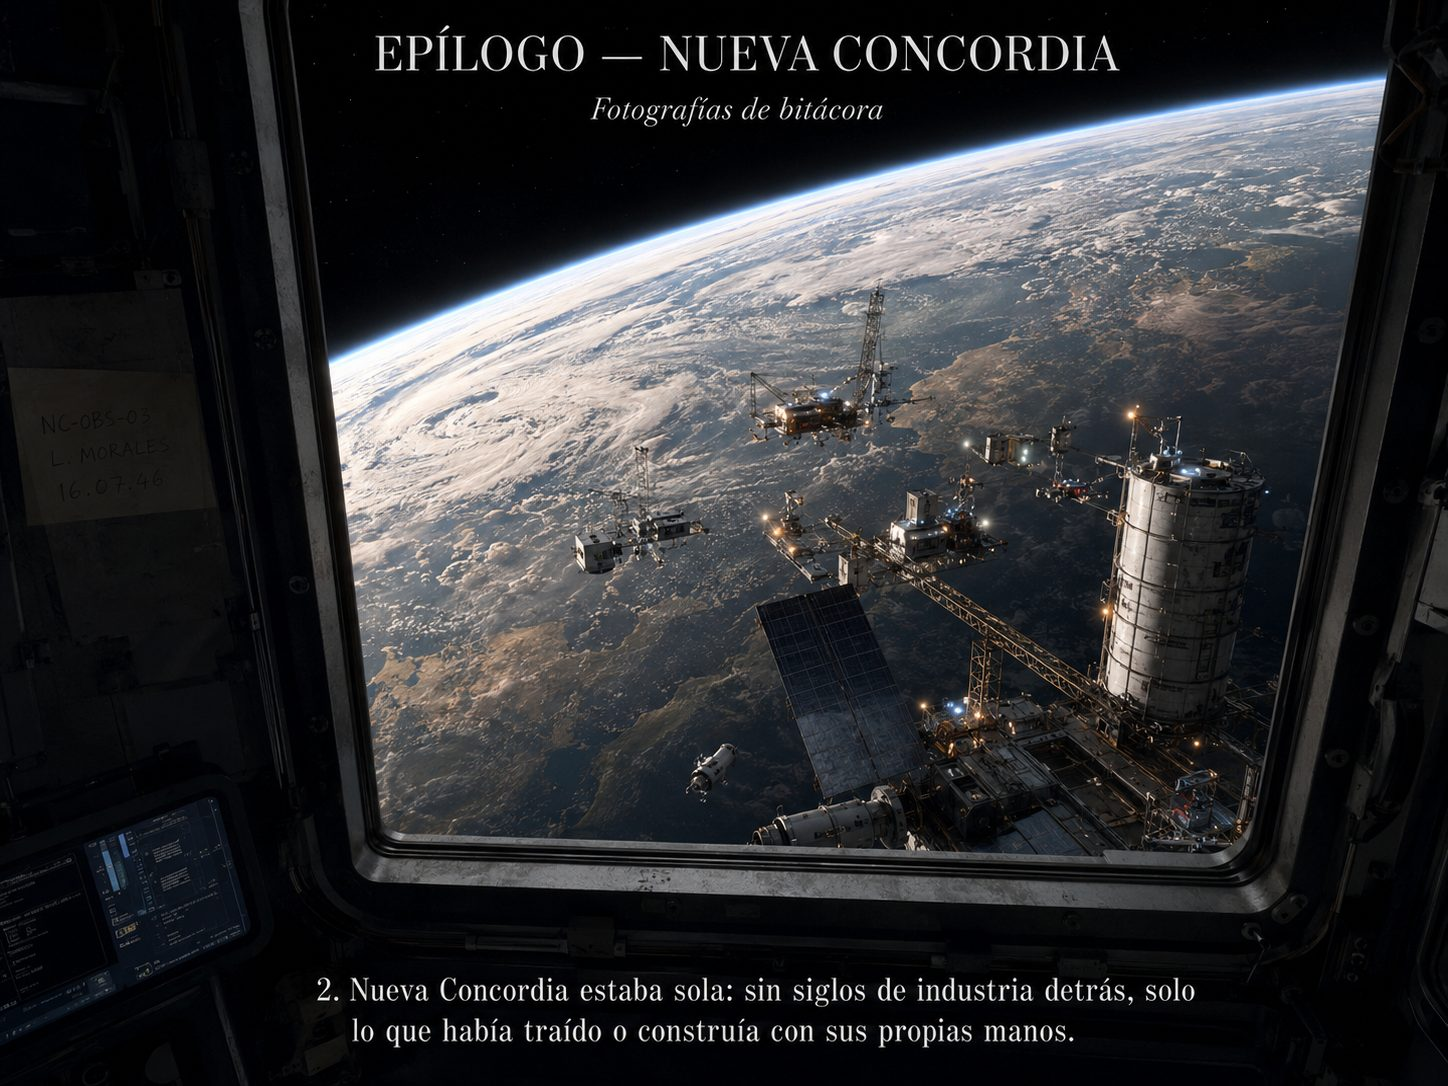
\includegraphics[width=0.9\textwidth]{12_3_eplogodelacoloniaespacialnuevaconcordia.jpg}
\end{figure}

Al aterrizar, la superficie vibró bajo nosotros. No mucho. Apenas un temblor, como cuando un edificio absorbe el impacto de algo grande y lo distribuye hacia abajo y hacia los lados con la resignación de los materiales que saben lo que tienen que hacer.

La puerta se abrió.

El aire exterior no era respirable, pero los sensores dijeron que la presión era estable, la temperatura tolerable dentro del traje y el viento moderado desde el noroeste, si es que el noroeste existía aquí todavía. Frente a mí había una explanada de roca oscura, más oscura que cualquier basalto terrestre, con torres de construcción al fondo y cúpulas presurizadas conectadas por túneles translúcidos. Más allá de las cúpulas, a donde alcanzaba la vista antes de que el horizonte curvado del planeta lo cortara todo, roca y más roca, y luego un amanecer de Alpha Centauri A que se extendía sobre todo eso con una luz ligeramente más dorada que la del Sol, como si alguien hubiera ajustado el balance de blancos del mundo.

\begin{figure}[h]
\centering
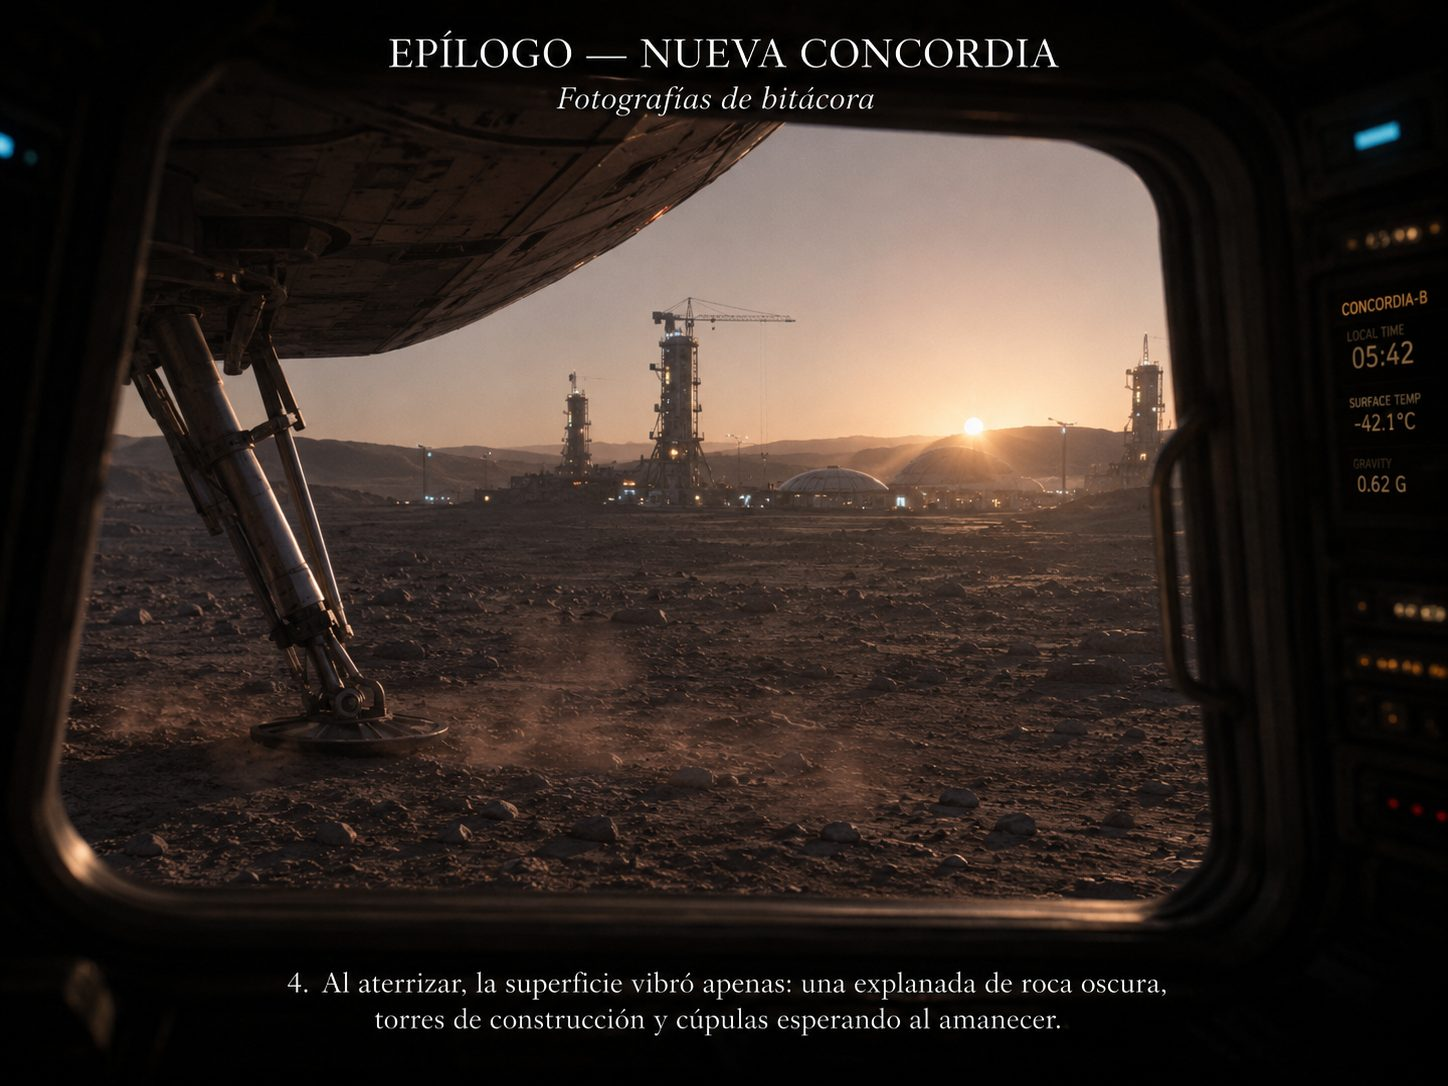
\includegraphics[width=0.9\textwidth]{12_4_epilogoennuevaconcordiaalaterrizar.jpg}
\end{figure}

Bajé por la rampa con el casco sellado.

\begin{figure}[h]
\centering
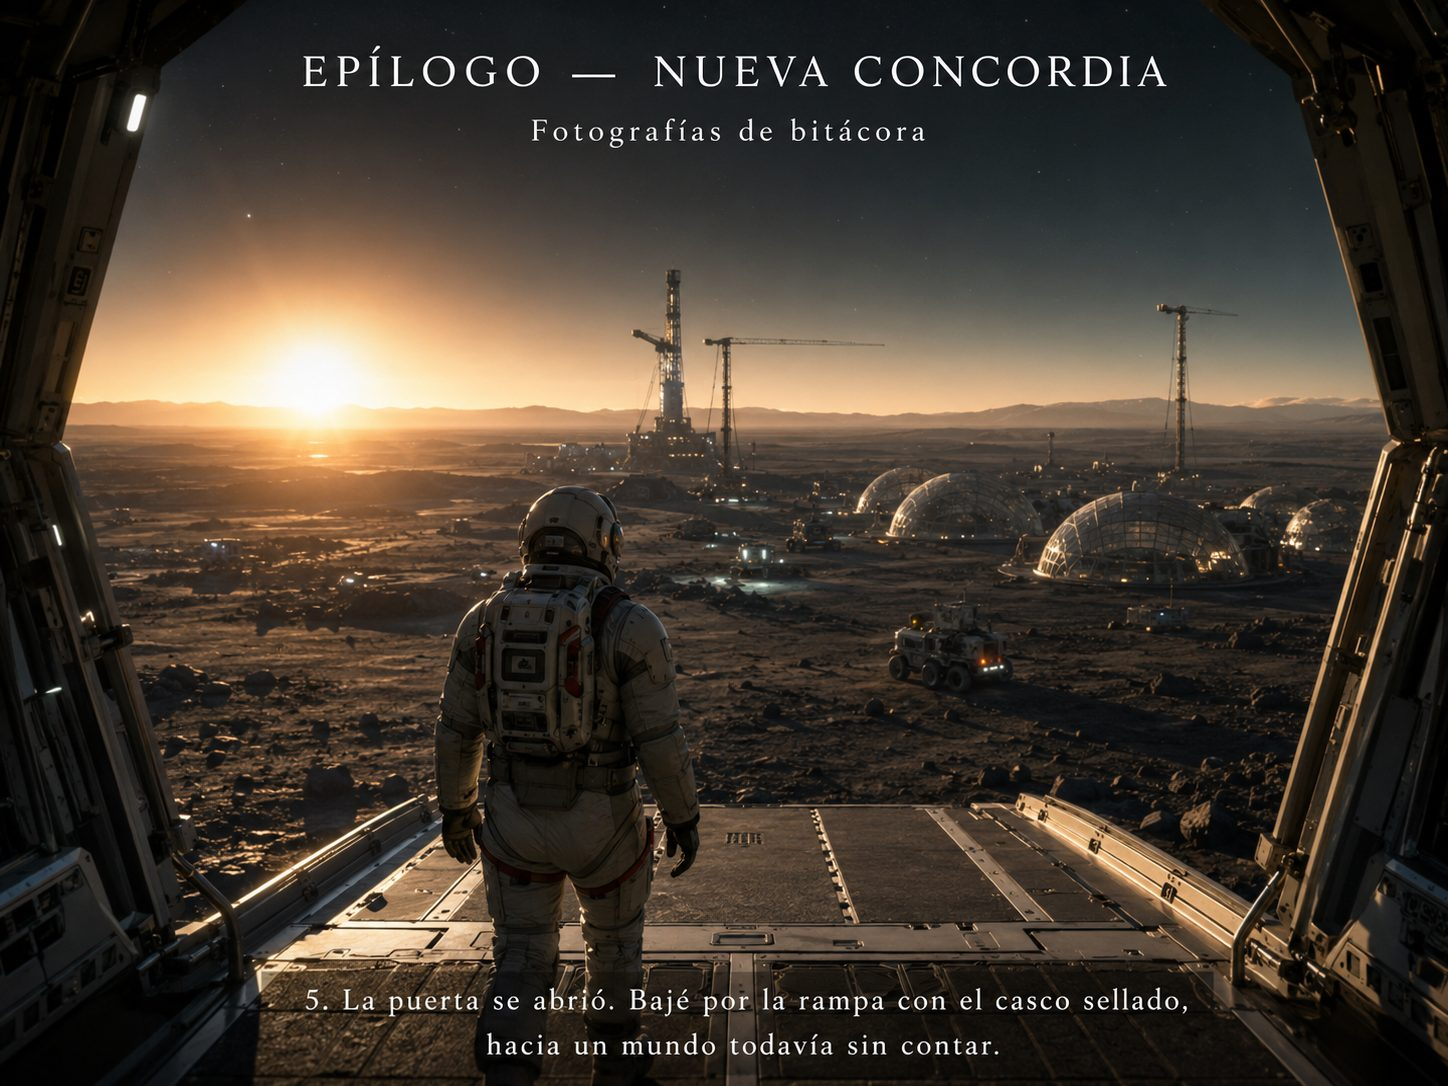
\includegraphics[width=0.9\textwidth]{12_5_amanecerenlacoloniaaliengenasalimosdelanave.jpg}
\end{figure}

Activé la grabadora.

—Diario de llegada, día uno. Nueva Concordia. He tardado un año en llegar hasta aquí, aunque quizá debería decir que he tardado toda una civilización. La Tierra ya no es el único principio. A partir de hoy, también es un origen.

\begin{figure}[h]
\centering
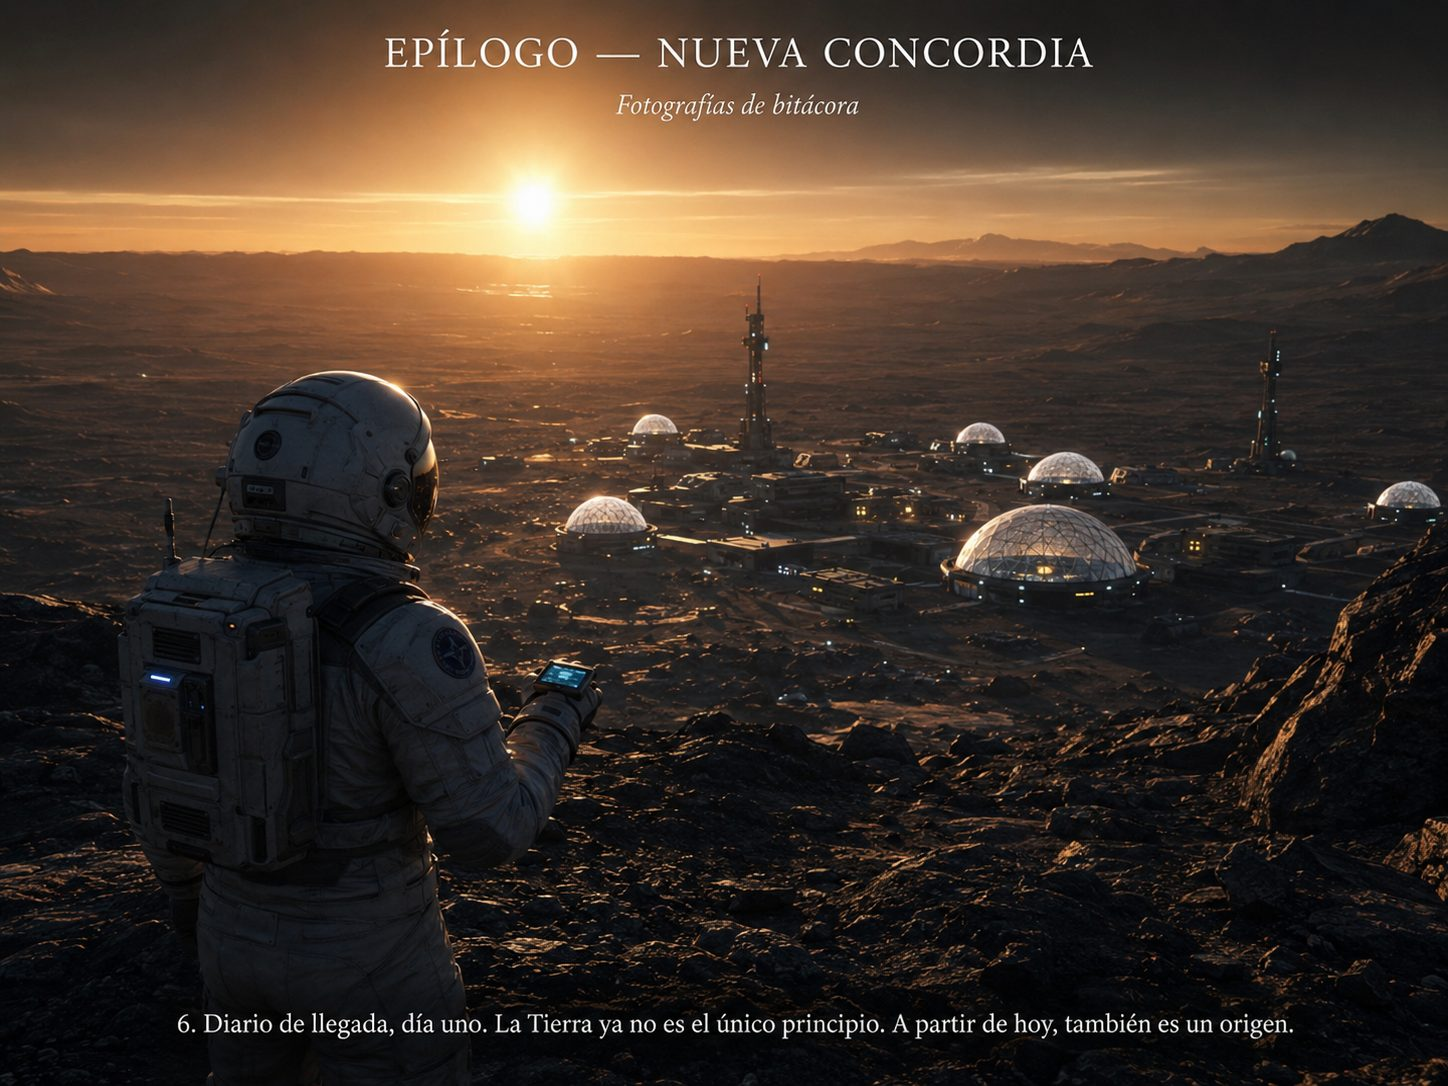
\includegraphics[width=0.9\textwidth]{12_6_eplogoennuevaconcordiadiariodellegadadia1.jpg}
\end{figure}

Hice una pausa. Había más que decir. Había un año entero que decir.

Pero lo guardaré para mañana. Y para el día siguiente. Y para todos los días que vienen, en este mundo que todavía no sabe que va a ser contado.

Y por primera vez desde que salí, no miré atrás.

\vspace{1.5em}
\begin{center}$\ast$\quad$\ast$\quad$\ast$\end{center}
\vspace{1.5em}

\textit{Fin}


\end{document}
